
%%%%%%%%%%%%%%%%%%%%%%%%%%%%%%%%%%%%%%%%%%%%%%%%%%%%%%%%%%%%%%%%%%%%%%
%%%%%%%%%%%%%%%%%%%%%%%%%%%%%%%%%%%%%%%%%%%%%%%%%%%%%%%%%%%%%%%%%%%%%
%%%%%%%%%%%%%%%%%%%%%%%%%%%%%%%%%%%%%%%%%%%%%%%%%%%%%%%%%%%%%%%%%%%%%
%%%%%%%%%%%%%%%%%%%%%%%%%%%%%%%%%%%%%%%%%%%%%%%%%%%%%%%%%%%%%%%%%%%%%

\chapter{Selected distributions in ProbOnto knowledge base}
\label{ch:probontoAppendix}

The full first version of ProbOnto will be released soon. Here we provide 
a brief overview of a part of its content for the most frequently used distributions 
and/or alternative parameterisations (38 out of about 55). 

The according plots have been performed using the R code stored in ProbOnto 
and provided for each distribution for which it's available.


%%%%%%%%%%%%%%%%%%%%%%%%%%%%%%%%%%%%%%%%%%%%%%%%%%%%%%%%%%%%%%%%%%%%%
\paragraph{Symbols used}
Some of the symbols used in definitions of the functions and quantities 
listed in the subsequent sections are collected here with references
\begin{itemize}
\item Beta function, $B$\\
\url{http://mathworld.wolfram.com/BetaFunction.html}\\
\url{http://en.wikipedia.org/wiki/Beta_function}
\item Regularized incomplete Beta function,  $I_p$, $I_{1-p}$\\
\url{http://mathworld.wolfram.com/RegularizedBetaFunction.html}\\
\url{http://en.wikipedia.org/wiki/Beta_function#Incomplete_beta_function}
\item Error function, $erf$\\
\url{http://mathworld.wolfram.com/Erf.html}\\
\url{https://en.wikipedia.org/wiki/Error_function}
\item Floor function, $\lfloor k \rfloor$\\
\url{http://mathworld.wolfram.com/FloorFunction.html}\\
\url{https://en.wikipedia.org/wiki/Floor_and_ceiling_functions}
\item Gamma function, $\Gamma$ \\
\url{http://mathworld.wolfram.com/GammaFunction.html}\\
\url{http://en.wikipedia.org/wiki/Gamma_function}
\item Lower incomplete gamma function, $\gamma$\\
\url{http://mathworld.wolfram.com/IncompleteGammaFunction.html}\\
\url{https://en.wikipedia.org/wiki/Incomplete_gamma_function}
\item Multivariate Gamma function,	$\Gamma_p$\\
\url{https://en.wikipedia.org/wiki/Multivariate_gamma_function}
\item Iverson bracket, $[x=i]$\\ 
\url{http://mathworld.wolfram.com/IversonBracket.html}\\
\url{http://en.wikipedia.org/wiki/Iverson_bracket}
\item Linear span, $span$\\
\url{http://mathworld.wolfram.com/VectorSpaceSpan.html}\\
\url{https://en.wikipedia.org/wiki/Linear_span}
\item (Generalized) Hypergeometric function, ($_pF_q$), $_2F_1$\\
\url{http://mathworld.wolfram.com/HypergeometricFunction.html}\\
\url{http://en.wikipedia.org/wiki/Hypergeometric_function}
\end{itemize}



%%%%%%%%%%%%%%%%%%%%%%%%%%%%%%%%%%%%%%%%%%%%%%%%%%%%%%%%%%%%%%%%%%%%%%%%%%%%%%%%%%%%%%%%%%%%%%%%%%%%%%%%%%%%%%%%%%%%%%%%%%%%%%%%%%%%%%%%%%%%%%%%%%%%%%%%%%%%%%%%%%%%%%%%%%%%%%%%%%%%%%%%%%%%%%%%%%%%%%%%%%%%%%%%%%%%%%%%%%%%%%%%%%%%%%%%%%%%%%%%%%%%%%%%%%%%%%%%%%%%%%%%%%%%%%%%%%%%%%%%%%%%%%%%%%%%%%%%%%%%%%%%%%%%%%%%%%%%%%%%%%%%
%\chapter{New version}

\section*{Bernoulli} 

  \bigskip 

\begin{tabular}{p{2cm}cl}
\textbf{name} & & Bernoulli (ID: 0000000)\\ 
 
\textbf{type} & & discrete \\ 

\textbf{variate} & & $k$, scalar \\ 

\textbf{support} & & $k \in \{0,1\}$
\end{tabular}

\begin{figure}[ht!]
\centering
  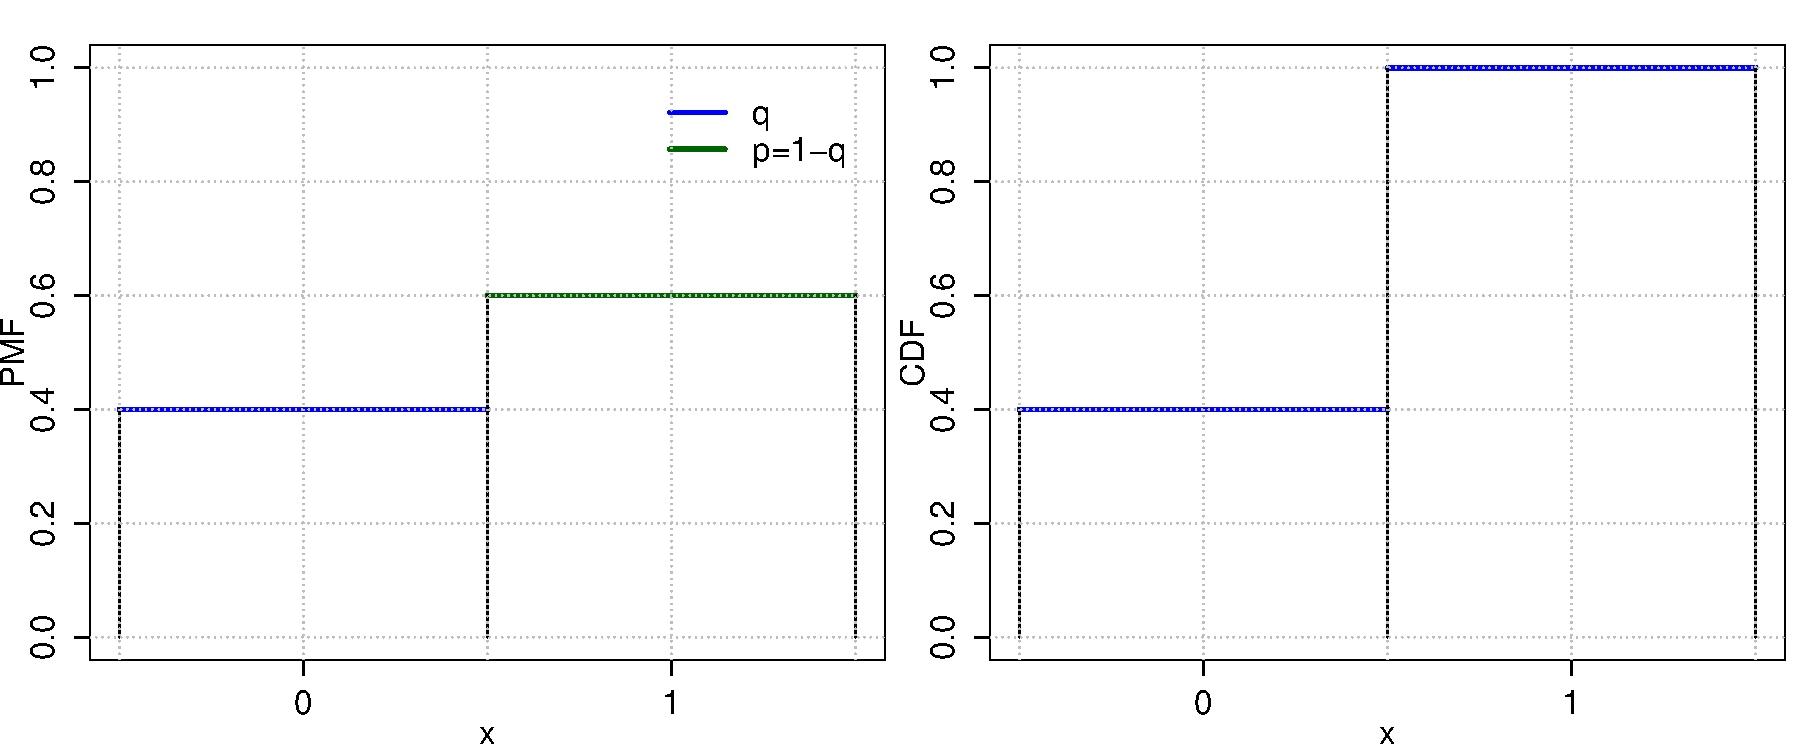
\includegraphics[width=140mm]{pics/Bernoulli_pmf_cdf.pdf}
 \caption{PDF and CDF of the Bernoulli distribution for p=0.6.}
 \label{fig:Bernoulli_pmf_cdf}
\end{figure}


\subsubsection*{Parameter: probability}

\noindent\begin{tabular}{p{2cm}cl}
\textbf{name} & & probability \\
\textbf{type} & & scalar \\
\textbf{symbol} & & $p$  \\
\textbf{definition} & & $0<p<1, p \in  R$
\end{tabular}
\subsubsection*{Functions}

\smallskip \noindent \hspace{.2cm} \textbf{PMF} 
\begin{equation*}\begin{cases}
    q=(1-p) & \text{for }k=0 \\ p & \text{for }k=1
    \end{cases}\end{equation*}
\smallskip \noindent \hspace{.2cm} \textbf{PMF in R}  
\begin{verbatim}q=(1-p) for k=0 \\
p for k=1\end{verbatim}
\smallskip \noindent \hspace{.2cm} \textbf{CDF} 
\begin{equation*}\begin{cases}
    0 & \text{for }k<0 \\ q & \text{for }0\leq k<1 \\ 1 & \text{for }k\geq 1
    \end{cases}\end{equation*}
\smallskip\section*{Beta} 

  \bigskip 

\begin{tabular}{p{2cm}cl}
\textbf{name} & & Beta (ID: 0000012)\\ 
 
\textbf{type} & & continuous \\ 

\textbf{variate} & & $x$, scalar \\ 

\textbf{support} & & $x \in (0,1)$
\end{tabular}

\begin{figure}[ht!]
\centering
  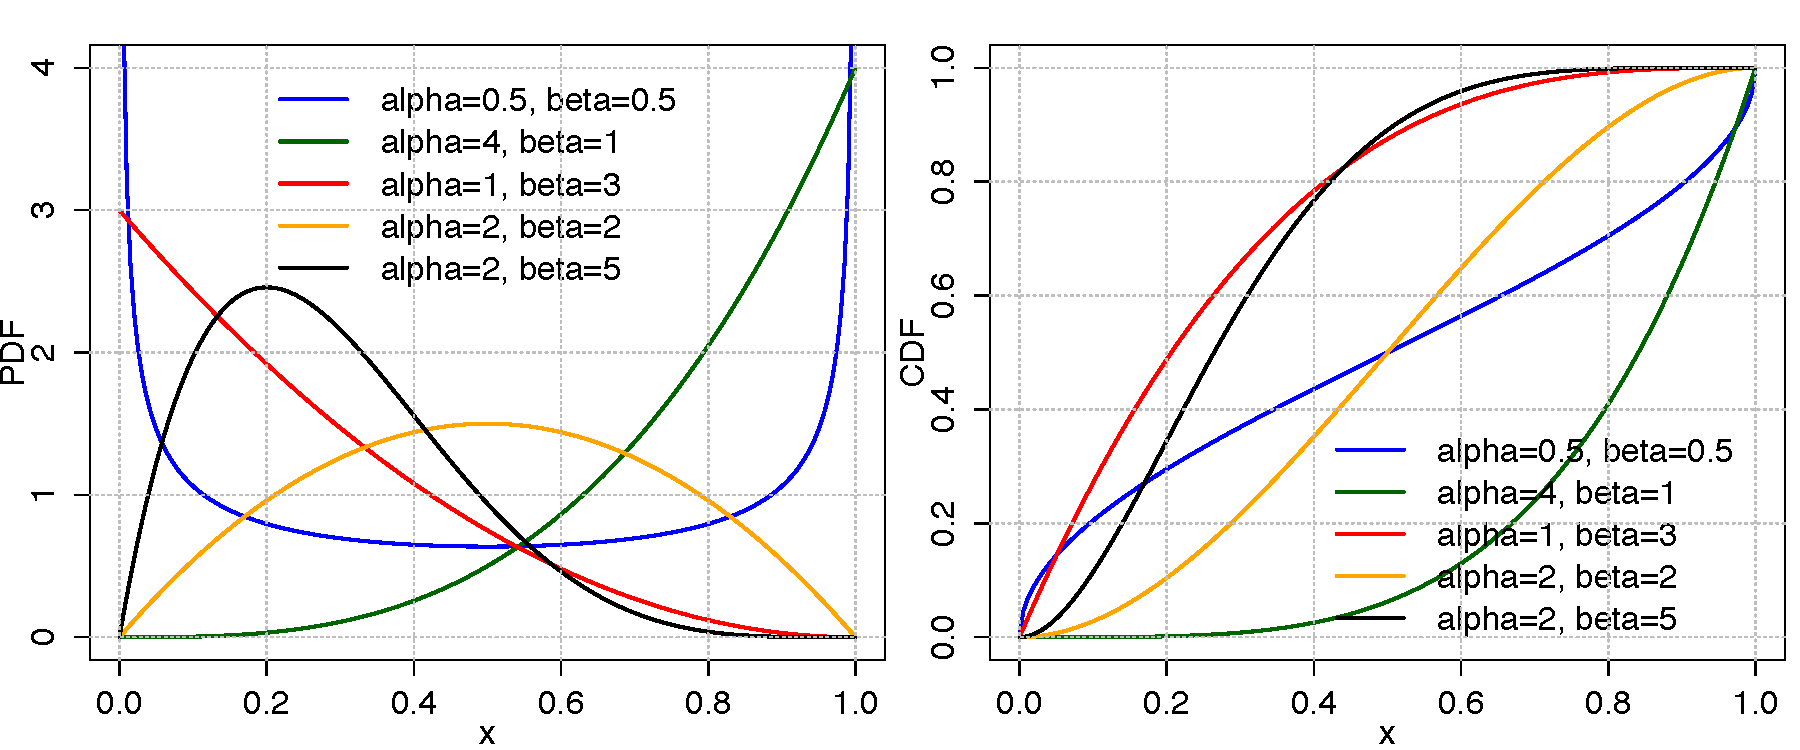
\includegraphics[width=140mm]{pics/Beta_pdf_cdf.pdf}
 \caption{PDF and CDF of the Beta distribution plotted using the provided R-code.}
 \label{fig:Beta_pdf_cdf}
\end{figure}

\subsubsection*{Parameter: alpha}

\noindent\begin{tabular}{p{2cm}cl}
\textbf{name} & & shape \\
\textbf{type} & & scalar \\
\textbf{symbol} & & $\alpha$  \\
\textbf{definition} & & $\alpha > 0$
\end{tabular}
\subsubsection*{Parameter: beta}

\noindent\begin{tabular}{p{2cm}cl}
\textbf{name} & & shape \\
\textbf{type} & & scalar \\
\textbf{symbol} & & $\beta$  \\
\textbf{definition} & & $\beta > 0$
\end{tabular}
\subsubsection*{Functions}

\smallskip \noindent \hspace{.2cm} \textbf{PDF} 
\begin{equation*}\frac{x^{\alpha-1}(1-x)^{\beta-1}} {B(\alpha,\beta)} \end{equation*}
\smallskip \noindent \hspace{.2cm} \textbf{PDF in R}  
\begin{verbatim}(x^(alpha-1)*(1-x)^(beta-1))/beta(alpha,beta)\end{verbatim}
\smallskip \noindent \hspace{.2cm} \textbf{CDF} 
\begin{equation*}I_x(\alpha,\beta)\end{equation*}
\smallskip \noindent \hspace{.2cm} \textbf{CDF in R} 
\begin{verbatim}Rbeta(x, a, b)\end{verbatim}
\smallskip\section*{Binomial} 

  \bigskip 

\begin{tabular}{p{2cm}cl}
\textbf{name} & & Binomial (ID: 0000024)\\ 
 
\textbf{type} & & discrete \\ 

\textbf{variate} & & $k$, scalar \\ 

\textbf{support} & & $k \in \{0,\dots,n\}$
\end{tabular}

\begin{figure}[htb!]
\centering
  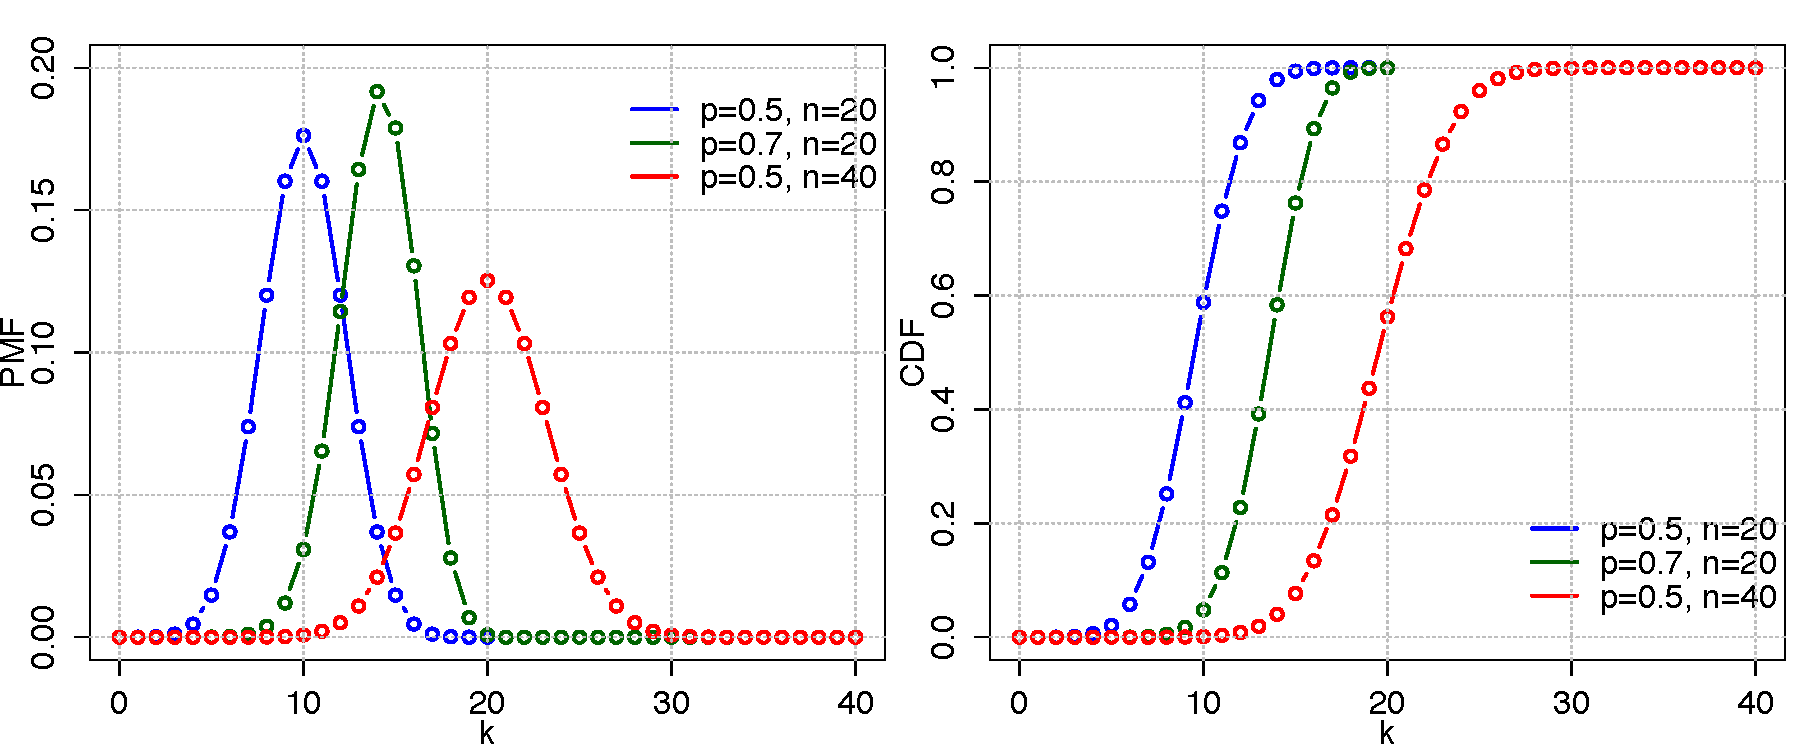
\includegraphics[width=140mm]{pics/Binomial_pmf_cdf.pdf}
 \caption{PMF and CDF of the Binomial distribution plotted using the provided R-code.}
 \label{fig:Bionomial_pmf_cdf}
\end{figure}

\subsubsection*{Parameter: numberOfFailures}

\noindent\begin{tabular}{p{2cm}cl}
\textbf{name} & & number of trials \\
\textbf{type} & & scalar \\
\textbf{symbol} & & $n$  \\
\textbf{definition} & & $n \in N, n \ge 0$
\end{tabular}
\subsubsection*{Parameter: probability}

\noindent\begin{tabular}{p{2cm}cl}
\textbf{name} & & success probability in each trial \\
\textbf{type} & & scalar \\
\textbf{symbol} & & $p$  \\
\textbf{definition} & & $p \in [0,1]$
\end{tabular}
\subsubsection*{Functions}

\smallskip \noindent \hspace{.2cm} \textbf{PMF} 
\begin{equation*}{n \choose k}\, p^k (1-p)^{n-k}\end{equation*}
\smallskip \noindent \hspace{.2cm} \textbf{PMF in R}  
\begin{verbatim}choose(n,k) * p^k*(1-p)^(n-k)\end{verbatim}
\smallskip \noindent \hspace{.2cm} \textbf{CDF} 
\begin{equation*}I_{1-p}(n - k, 1 + k)\end{equation*}
\smallskip \noindent \hspace{.2cm} \textbf{CDF in R} 
\begin{verbatim}Rbeta(1-p, n-k, 1+k)\end{verbatim}
\smallskip\section*{BirnbaumSaunders} 

  \bigskip 

\begin{tabular}{p{2cm}cl}
\textbf{name} & & Birnbaum-Saunders (ID: 0000034)\\ 
 
\textbf{type} & & continuous \\ 

\textbf{variate} & & $x$, scalar \\ 

\textbf{support} & & $x \in [0,+\infty)$
\end{tabular}

\begin{figure}[htb!]
\centering
  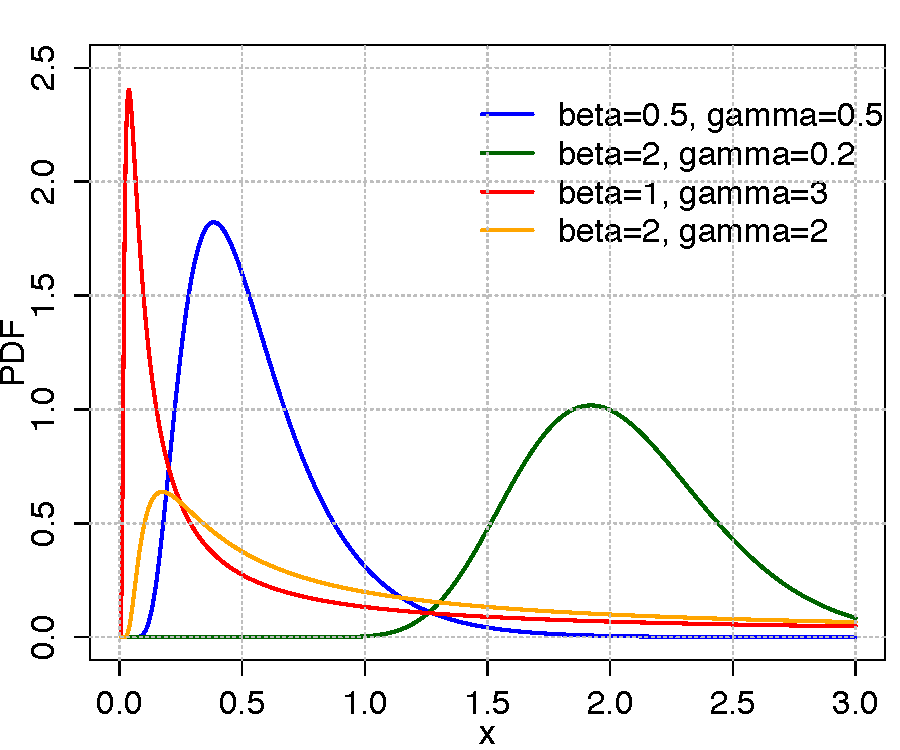
\includegraphics[width=70mm]{pics/BirnbaumSaunders_pdf.pdf}
 \caption{PDF of the Birnbaum-Saunders distribution plotted using the provided R-code -- {\color{red} \scshape{find CDF}}.}
 \label{fig:BirnbaumSaunders_pdf}
\end{figure}

\subsubsection*{Parameter: scale}

\noindent\begin{tabular}{p{2cm}cl}
\textbf{name} & & scale \\
\textbf{type} & & scalar \\
\textbf{symbol} & & $\beta$  \\
\textbf{definition} & & $\beta > 0$
\end{tabular}
\subsubsection*{Parameter: shape}

\noindent\begin{tabular}{p{2cm}cl}
\textbf{name} & & shape \\
\textbf{type} & & scalar \\
\textbf{symbol} & & $\gamma$  \\
\textbf{definition} & & $\gamma > 0$
\end{tabular}
\subsubsection*{Functions}

\smallskip \noindent \hspace{.2cm} \textbf{PDF} 
\begin{equation*}\frac{1}{\sqrt{2\pi}}\exp\Big[-\frac{(\sqrt{x/\beta}-\sqrt{\beta/x})^2}{2\gamma^2}\Big]\Big[\frac{\sqrt{x/\beta}+\sqrt{\beta/x}}{2\gamma x}\Big]\end{equation*}
\smallskip \noindent \hspace{.2cm} \textbf{PDF in R}  
\begin{verbatim}1/(sqrt(2*pi))* exp( -(sqrt(x/beta) - sqrt(beta/x))^2 / (2*gamma^2) ) 
			* ( sqrt(x/beta) + sqrt(beta/x) ) / (2*gamma*x)
\end{verbatim}
\smallskip \noindent \hspace{.2cm} \textbf{CDF} 
\begin{equation*}-\end{equation*}
\smallskip\section*{CategoricalNonordered} 

  \bigskip 

\begin{tabular}{p{2cm}cl}
\textbf{name} & & Categorical Nonordered (ID: 0000053)\\ 
 
\textbf{type} & & discrete \\ 

\textbf{variate} & & $x$, scalar \\ 

\textbf{support} & & $x \in \{1,\dots,k\}$
\end{tabular}

\begin{figure}[htb!]
\centering
  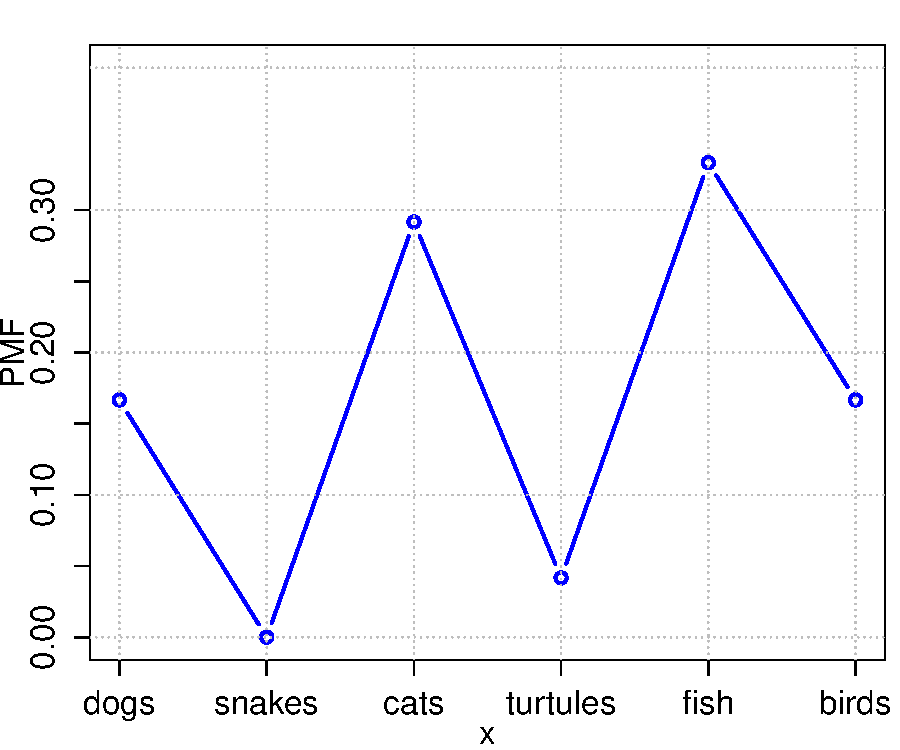
\includegraphics[width=70mm]{pics/CategoricalUnOrdered_pmf_cdf.pdf}
 \caption{An example for a PMF of the Categorical Unordered distribution for pets owned by children, with probabilities for each category \{0.17, 0, 0.29, 0.042, 0.33, 0.167\}. In this case the CDF is undefined.}
 \label{fig:CategoricalUnOrdered_pmf_cdf}
\end{figure}

\subsubsection*{Parameter: categoryProb}

\noindent\begin{tabular}{p{2cm}cl}
\textbf{name} & & category probabilities \\
\textbf{type} & & vector \\
\textbf{symbol} & & $p_1, \ldots, p_k$  \\
\textbf{definition} & & $0 \leq p_i \leq 1, \Sigma p_i = 1$
\end{tabular}
\subsubsection*{Functions}

\smallskip \noindent \hspace{.2cm} \textbf{PMF} 
\begin{equation*}p(x=i)=p_i\end{equation*}
\smallskip \noindent \hspace{.2cm} \textbf{CDF} 
\begin{equation*}undefined\end{equation*}
\smallskip\section*{CategoricalOrdered} 

  \bigskip 

\begin{tabular}{p{2cm}cl}
\textbf{name} & & Categorical Ordered (ID: 0000044)\\ 
 
\textbf{type} & & discrete \\ 

\textbf{variate} & & $x$, scalar \\ 

\textbf{support} & & $x \in \{1,\dots,k\}$
\end{tabular}

\begin{figure}[htb!]
\centering
  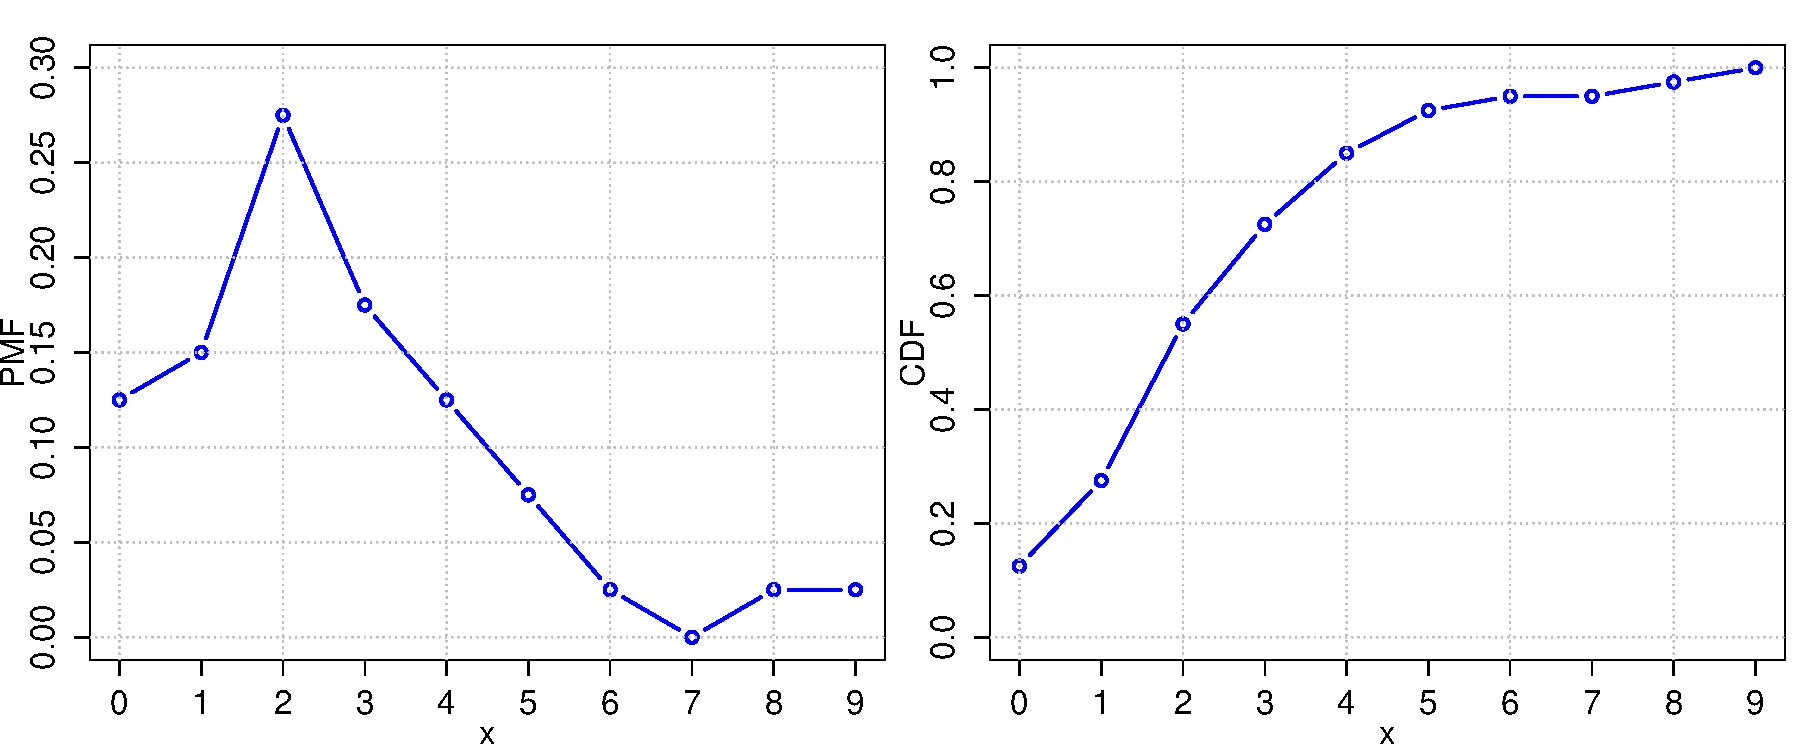
\includegraphics[width=140mm]{pics/CategoricalOrdered_pmf_cdf.pdf}
 \caption{An example for a PMF and CDF of the Categorical Ordered distribution 
 plotted using the provided R-code. Using data from \url{https://onlinecourses.science.psu.edu/stat414/node/13}}
 \label{fig:CategoricalOrdered_pmf_cdf}
\end{figure}

\subsubsection*{Parameter: categoryProb}

\noindent\begin{tabular}{p{2cm}cl}
\textbf{name} & & category probabilities \\
\textbf{type} & & vector \\
\textbf{symbol} & & $p_1, \ldots, p_k$  \\
\textbf{definition} & & $0 \leq p_i \leq 1, \Sigma p_i = 1$
\end{tabular}
\subsubsection*{Functions}

\smallskip \noindent \hspace{.2cm} \textbf{PMF} 
\begin{equation*}p(x=i)=p_i\end{equation*}
\smallskip \noindent \hspace{.2cm} \textbf{CDF} 
\begin{equation*}\begin{cases}
    0 & \text{for }x<1 \\
    \sum_{j=1}^i p_j & \text{for }x \in [i,i+1) \\
    1 & \text{for }x \geq k
    \end{cases}\end{equation*}
\smallskip\section*{Cauchy} 

  \bigskip 

\begin{tabular}{p{2cm}cl}
\textbf{name} & & Cauchy (ID: 0000062)\\ 
 
\textbf{type} & & continuous \\ 

\textbf{variate} & & $x$, scalar \\ 

\textbf{support} & & $x \in (-\infty,+\infty)$
\end{tabular}

\begin{figure}[htb!]
\centering
  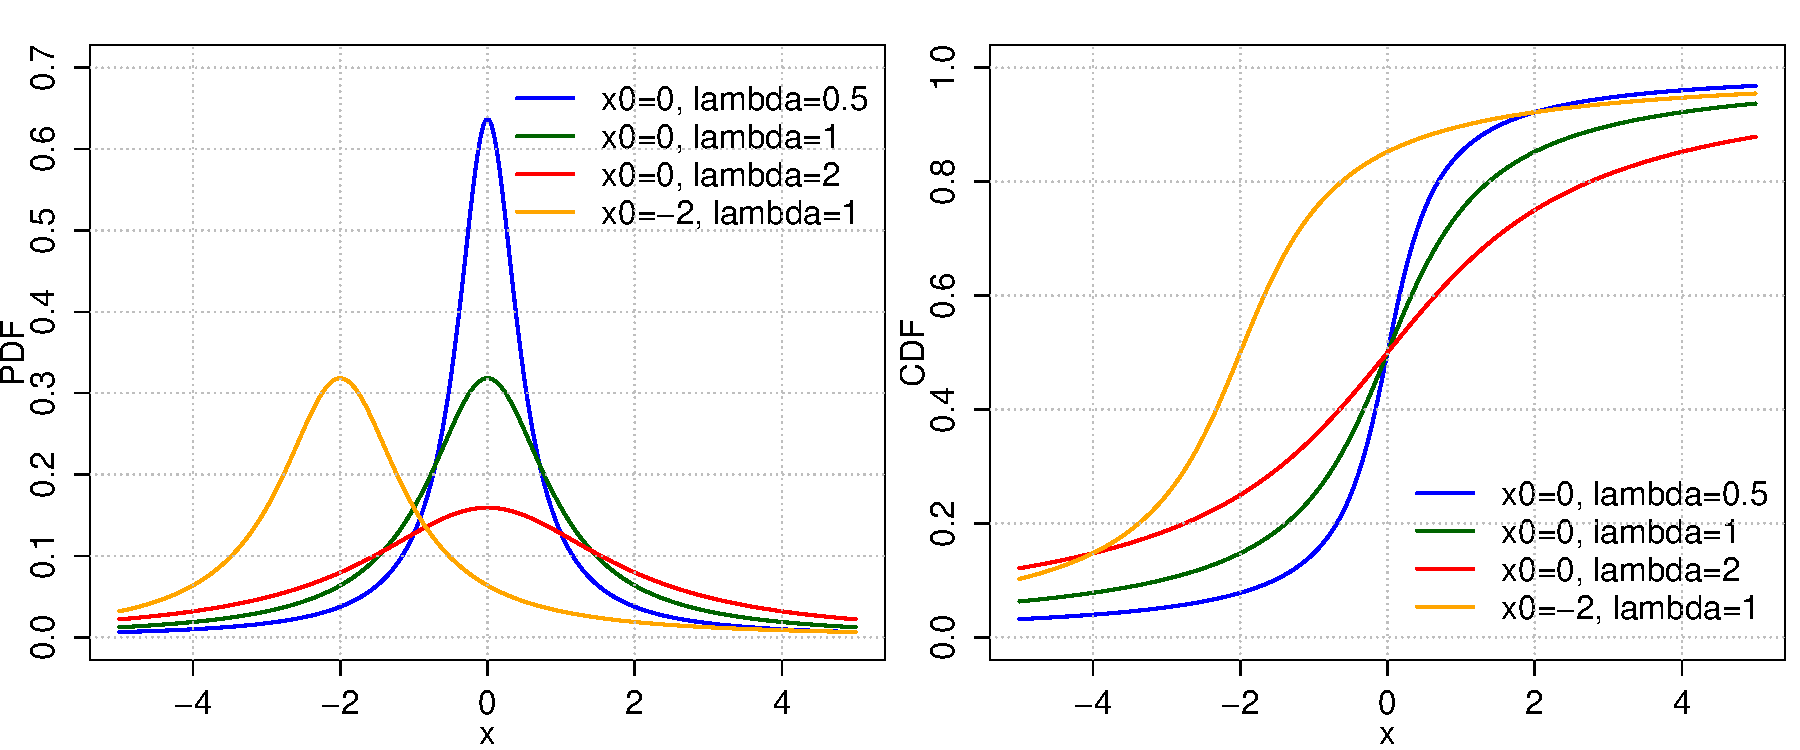
\includegraphics[width=140mm]{pics/Cauchy_pdf_cdf.pdf}
 \caption{PDF and CDF of the Cauchy distribution plotted using the provided R-code.}
 \label{fig:Cauchy_pdf_cdf}
\end{figure}

\subsubsection*{Parameter: location}

\noindent\begin{tabular}{p{2cm}cl}
\textbf{name} & & location \\
\textbf{type} & & scalar \\
\textbf{symbol} & & $x_0$  \\
\textbf{definition} & & $x_0 \in  R$
\end{tabular}
\subsubsection*{Parameter: scale}

\noindent\begin{tabular}{p{2cm}cl}
\textbf{name} & & scale \\
\textbf{type} & & scalar \\
\textbf{symbol} & & $\gamma$  \\
\textbf{definition} & & $\gamma \in  R$
\end{tabular}
\subsubsection*{Functions}

\smallskip \noindent \hspace{.2cm} \textbf{PDF} 
\begin{equation*}\frac{1}{\pi\gamma\,\left[1 + \left(\frac{x-x_0}{\gamma}\right)^2\right]}\end{equation*}
\smallskip \noindent \hspace{.2cm} \textbf{PDF in R}  
\begin{verbatim}1 / (pi*gamma*(1 + ((x-x0)^2/gamma^2)))\end{verbatim}
\smallskip \noindent \hspace{.2cm} \textbf{CDF} 
\begin{equation*}\frac{1}{\pi} \arctan\left(\frac{x-x_0}{\gamma}\right)+\frac{1}{2}\end{equation*}
\smallskip \noindent \hspace{.2cm} \textbf{CDF in R} 
\begin{verbatim}1/pi * atan((x-x0)/gamma)+1/2\end{verbatim}
\smallskip\section*{ChiSquared} 

  \bigskip 

\begin{tabular}{p{2cm}cl}
\textbf{name} & & Chi-squared (ID: 0000072)\\ 
 
\textbf{type} & & continuous \\ 

\textbf{variate} & & $x$, scalar \\ 

\textbf{support} & & $x \in [0,+\infty)$
\end{tabular}

\begin{figure}[htb!]
\centering
  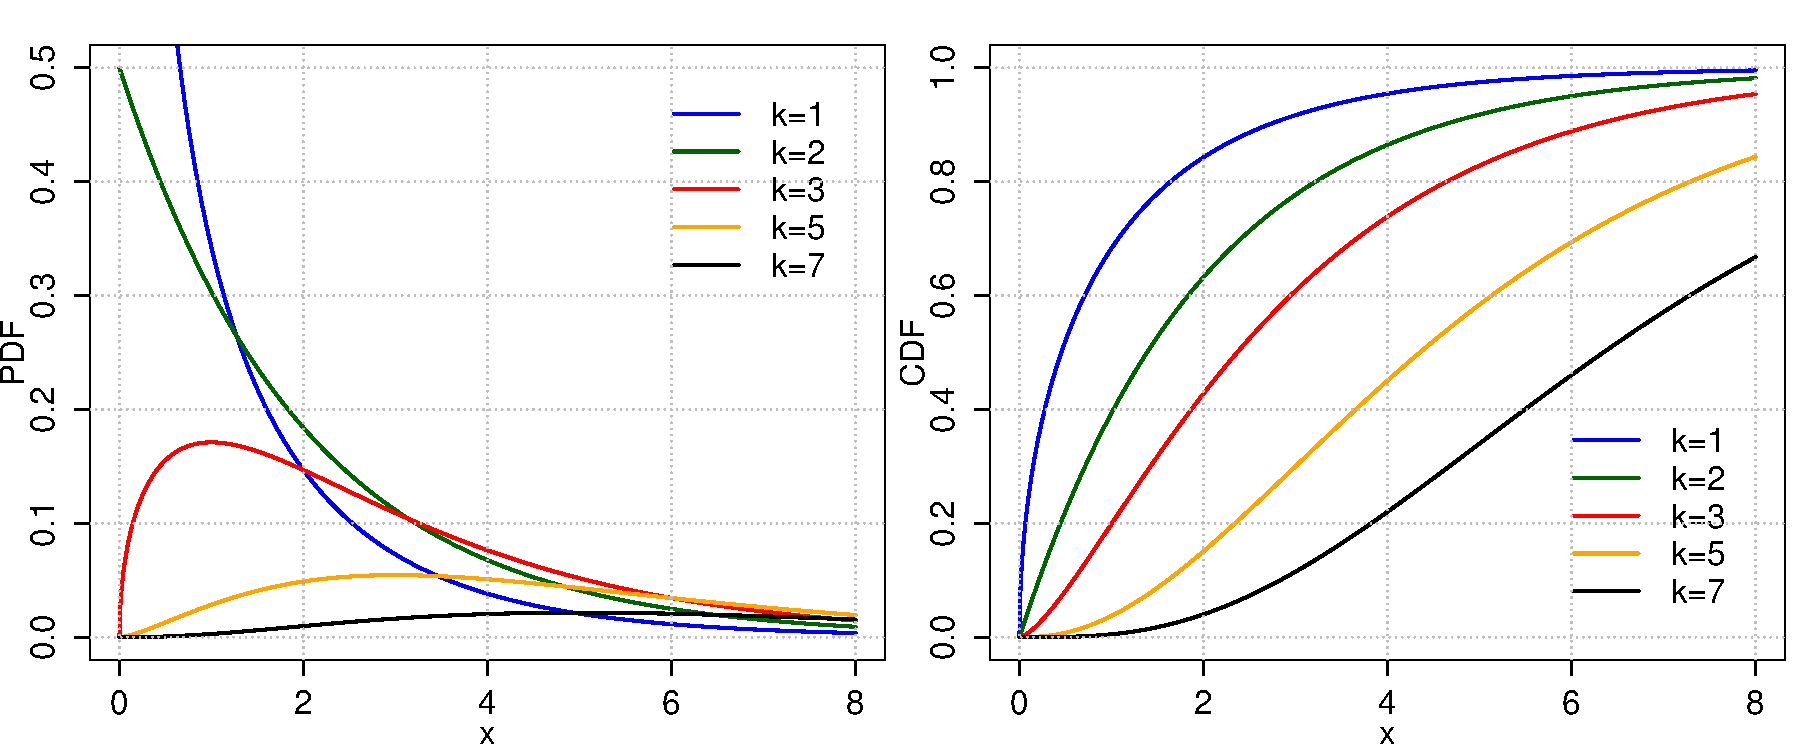
\includegraphics[width=140mm]{pics/ChiSquared_pdf_cdf.pdf}
 \caption{PDF and CDF of the Chi-squared distribution plotted using the provided R-code.}
 \label{fig:ChiSquared_pdf_cdf}
\end{figure}

\subsubsection*{Parameter: degreesOfFreedom}

\noindent\begin{tabular}{p{2cm}cl}
\textbf{name} & & degrees of freedom \\
\textbf{type} & & scalar \\
\textbf{symbol} & & $k$  \\
\textbf{definition} & & $k \in N$
\end{tabular}
\subsubsection*{Functions}

\smallskip \noindent \hspace{.2cm} \textbf{PDF} 
\begin{equation*}\frac{1}{2^{\frac{k}{2}}\Gamma\left(\frac{k}{2}\right)}\; x^{\frac{k}{2}-1} e^{-\frac{x}{2}}\end{equation*}
\smallskip \noindent \hspace{.2cm} \textbf{PDF in R}  
\begin{verbatim}1/( 2^k/2 * gamma(k/2) ) *  x^(k/2-1) * exp(-x/2)\end{verbatim}
\smallskip \noindent \hspace{.2cm} \textbf{CDF} 
\begin{equation*}\frac{1}{\Gamma\left(\frac{k}{2}\right)}\; \gamma\left(\frac{k}{2},\,\frac{x}{2}\right)\end{equation*}
\smallskip \noindent \hspace{.2cm} \textbf{CDF in R} 
\begin{verbatim}1/gamma(k/2) * Igamma(k/2,x/2)\end{verbatim}
%\smallskip\section*{DiracDelta} 
%
%  \bigskip 
%
%\begin{tabular}{p{2cm}cl}
%\textbf{name} & & Dirac Delta (ID: 0000082)\\ 
% 
%\textbf{type} & &  \\ 
%
%\textbf{variate} & & $-$, - \\ 
%
%\textbf{support} & & $-$
%\end{tabular}
%\subsubsection*{Functions}
%
%\smallskip \noindent \hspace{.2cm} \textbf{} 
%\begin{equation*}\end{equation*}
%\smallskip \noindent \hspace{.2cm} \textbf{CDF} 
%\begin{equation*}-\end{equation*}
\smallskip\section*{Dirichlet} 

  \bigskip 

\begin{tabular}{p{2cm}cl}
\textbf{name} & & Dirichlet (ID: 0000090)\\ 
 
\textbf{type} & & continuous \\ 

\textbf{variate} & & $x$, vector \\ 

\textbf{support} & & $x_1, \cdots, x_K \quad\text{where}\quad x_i \in [0,1]\quad and \quad\sum_{i=1}^K x_i = 1$
\end{tabular}
\subsubsection*{Parameter: concentration}

\noindent\begin{tabular}{p{2cm}cl}
\textbf{name} & & concentration \\
\textbf{type} & & vector \\
\textbf{symbol} & & $\alpha_1, \cdots, \alpha_K$  \\
\textbf{definition} & & $\alpha_1, \cdots, \alpha_K, \alpha_i > 0$
\end{tabular}
\subsubsection*{Functions}

\smallskip \noindent \hspace{.2cm} \textbf{PDF} 
\begin{equation*}\frac{1}{B(\alpha)} \prod_{i=1}^K x_i^{\alpha_i - 1} \\ \text{where} \quad B(\alpha) = \frac{\prod_{i=1}^K \Gamma(\alpha_i)}{\Gamma\bigl(\sum_{i=1}^K \alpha_i\bigr)} \\ \text{where} \quad \alpha=(\alpha_1,\ldots,\alpha_K)\end{equation*}
\smallskip \noindent \hspace{.2cm} \textbf{CDF} 
\begin{equation*}-\end{equation*}
\smallskip\section*{Exponential} 

  \bigskip 

\begin{tabular}{p{2cm}cl}
\textbf{name} & & Exponential (ID: 0000099)\\ 
 
\textbf{type} & & continuous \\ 

\textbf{variate} & & $x$, scalar \\ 

\textbf{support} & & $x \in [0,+\infty)$
\end{tabular}

\begin{figure}[ht!]
\centering
  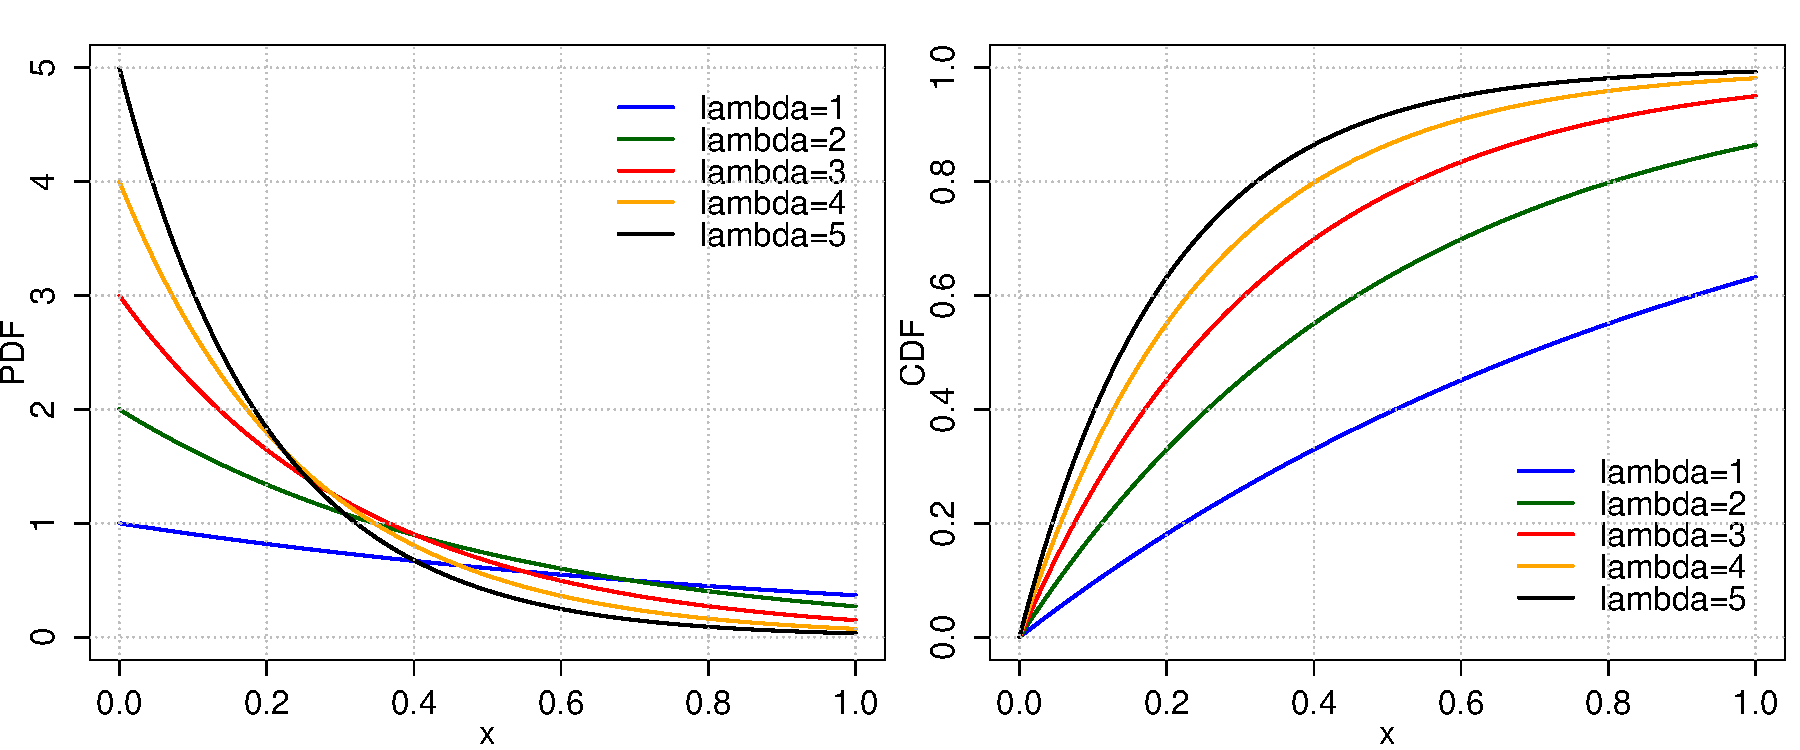
\includegraphics[width=140mm]{pics/Exponential_pdf_cdf.pdf}
 \caption{PDF and CDF of the Exponential distribution plotted using the provided R-code.}
 \label{fig:Exponential_pdf_cdf}
\end{figure}

\subsubsection*{Parameter: rate}

\noindent\begin{tabular}{p{2cm}cl}
\textbf{name} & & rate or inverse scale \\
\textbf{type} & & scalar \\
\textbf{symbol} & & $\lambda$  \\
\textbf{definition} & & $\lambda > 0$
\end{tabular}
\subsubsection*{Functions}

\smallskip \noindent \hspace{.2cm} \textbf{PDF} 
\begin{equation*}\lambda e^{-\lambda x}\end{equation*}
\smallskip \noindent \hspace{.2cm} \textbf{PDF in R}  
\begin{verbatim}lambda*exp(-lambda*x)\end{verbatim}
\smallskip \noindent \hspace{.2cm} \textbf{CDF} 
\begin{equation*}1 - e^{-\lambda x}\end{equation*}
\smallskip \noindent \hspace{.2cm} \textbf{CDF in R} 
\begin{verbatim}1 - exp(-lambda*x)\end{verbatim}
\smallskip\section*{F} 

  \bigskip 

\begin{tabular}{p{2cm}cl}
\textbf{name} & & F (ID: 0000108)\\ 
 
\textbf{type} & & continuous \\ 

\textbf{variate} & & $x$, scalar \\ 

\textbf{support} & & $x \in [0,+\infty)$
\end{tabular}

\begin{figure}[ht!]
\centering
  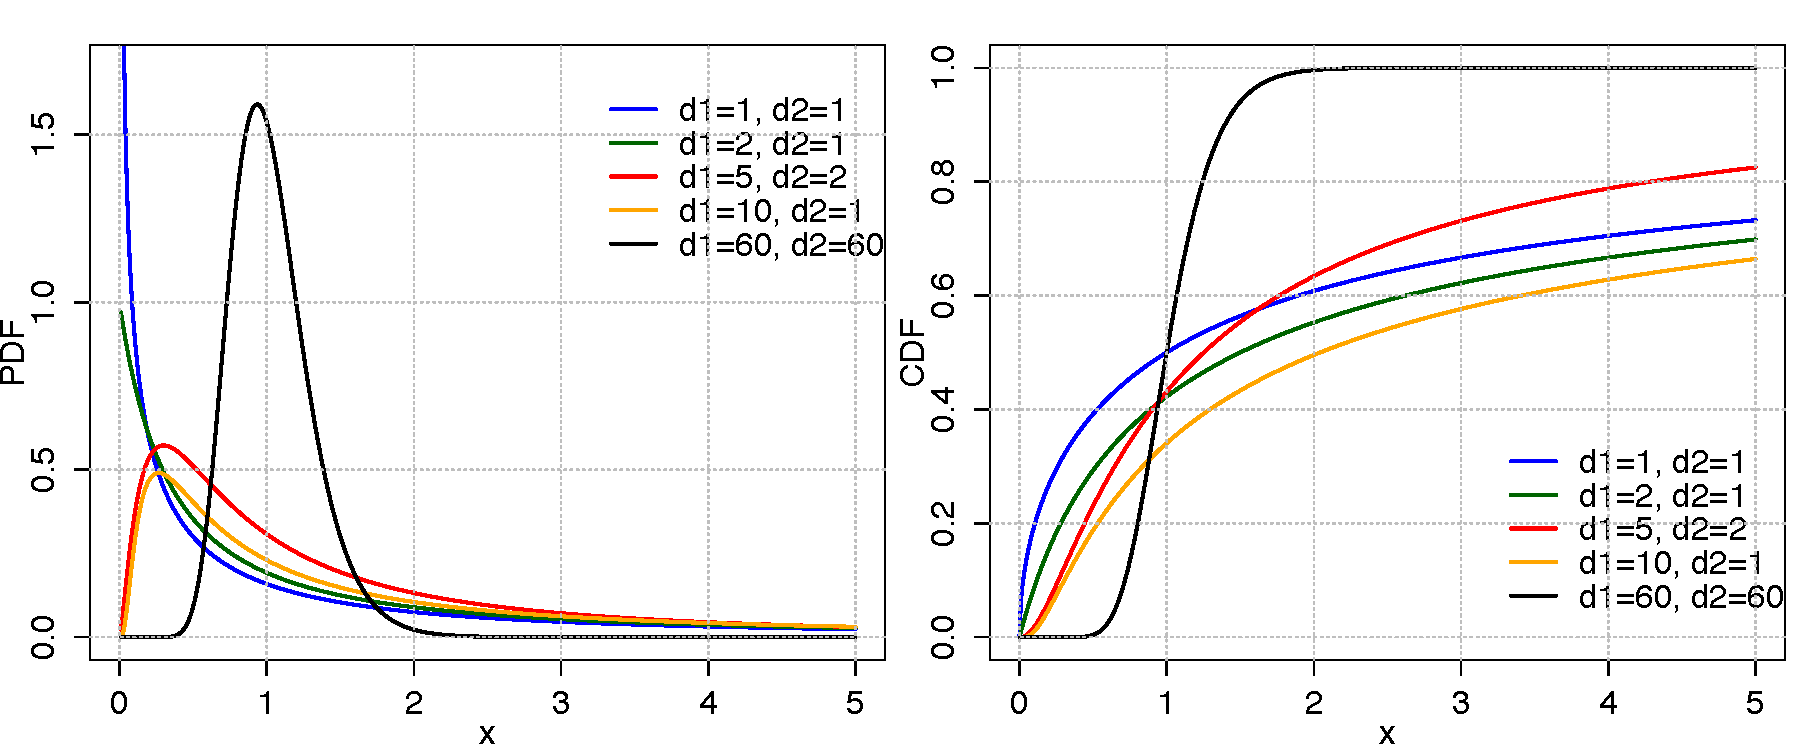
\includegraphics[width=140mm]{pics/F_pdf_cdf.pdf}
 \caption{PDF and CDF of the F distribution plotted using the provided R-code.}
 \label{fig:F_pdf_cdf}
\end{figure}

\subsubsection*{Parameter: numerator}

\noindent\begin{tabular}{p{2cm}cl}
\textbf{name} & & degree of freedom \\
\textbf{type} & & scalar \\
\textbf{symbol} & & $d_1$  \\
\textbf{definition} & & $d_1 > 0$
\end{tabular}
\subsubsection*{Parameter: denominator}

\noindent\begin{tabular}{p{2cm}cl}
\textbf{name} & & degree of freedom \\
\textbf{type} & & scalar \\
\textbf{symbol} & & $d_2$  \\
\textbf{definition} & & $d_2 > 0$
\end{tabular}
\subsubsection*{Functions}

\smallskip \noindent \hspace{.2cm} \textbf{PDF} 
\begin{equation*}\frac{\sqrt{\frac{(d_1 x)^{d_1}d_2^{d_2}}
{(d_1 x+d_2)^{d_1+d_2}}}}
{x B\left(\frac{d_1}{2},\frac{d_2}{2}\right)}\end{equation*}
\smallskip \noindent \hspace{.2cm} \textbf{PDF in R}  
\begin{verbatim}sqrt((d1*x)^d1*d2^(d2) / (d1*x+d2)^(d1+d2) ) / (x*beta(d1/2,d2/2))\end{verbatim}
\smallskip \noindent \hspace{.2cm} \textbf{CDF} 
\begin{equation*}I_{\frac{d_1 x}{d_1 x + d_2}} \left(\tfrac{d_1}{2}, \tfrac{d_2}{2} \right)\end{equation*}
\smallskip \noindent \hspace{.2cm} \textbf{CDF in R} 
\begin{verbatim}Rbeta(d1*x / (d1*x + d2), d1/2, d2/2)\end{verbatim}
\smallskip\section*{Gamma} 

  \bigskip 

\begin{tabular}{p{2cm}cl}
\textbf{name} & & Gamma (ID: 0000118)\\ 
 
\textbf{type} & & continuous \\ 

\textbf{variate} & & $x$, scalar \\ 

\textbf{support} & & $x \in (0,+\infty)$
\end{tabular}

\begin{figure}[ht!]
\centering
  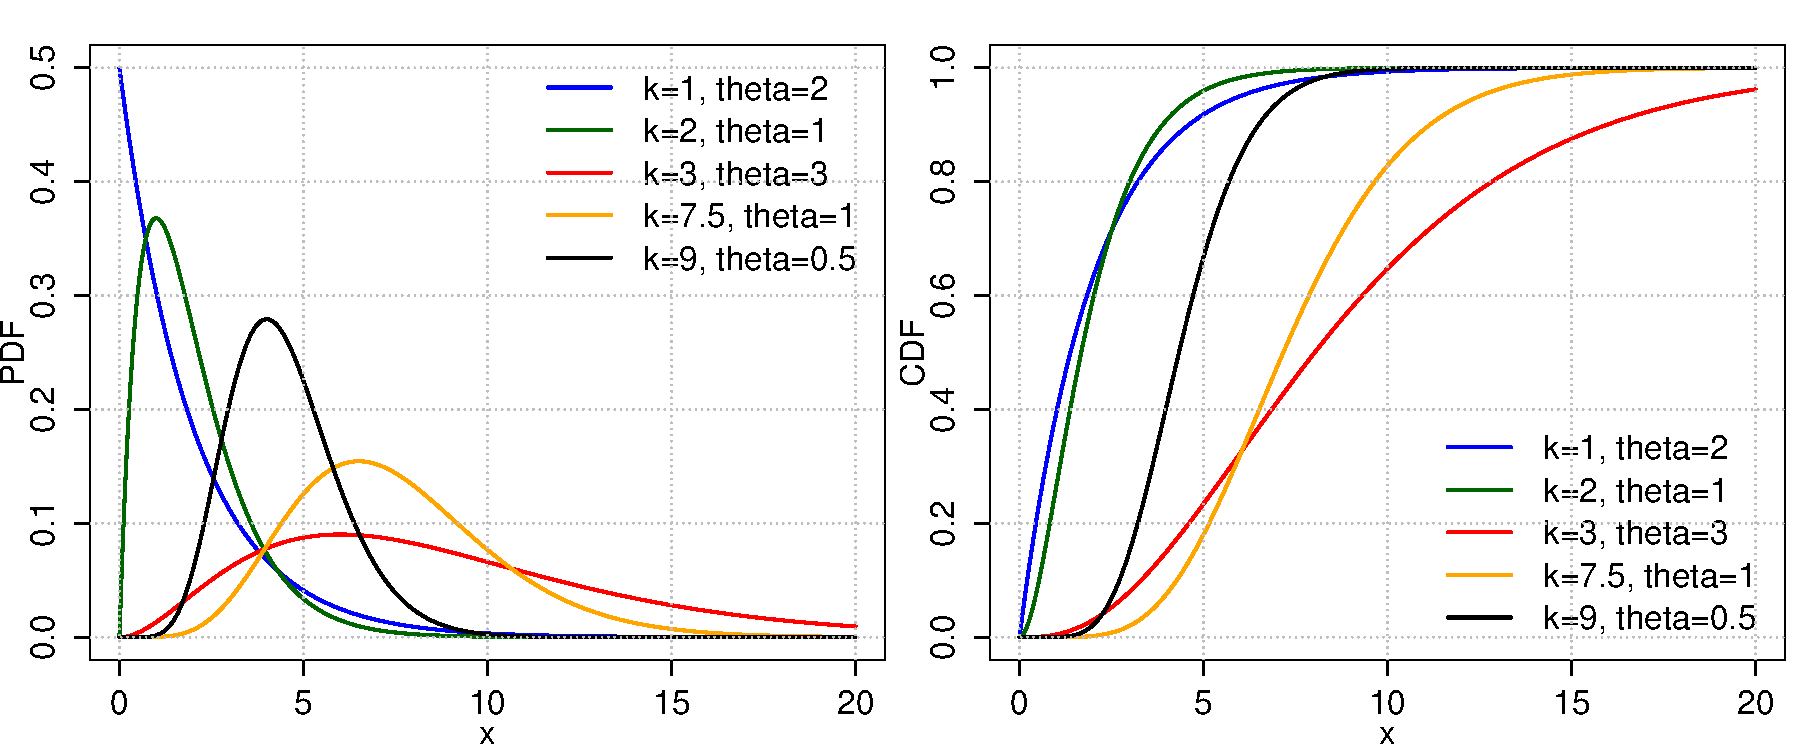
\includegraphics[width=140mm]{pics/Gamma_pdf_cdf.pdf}
 \caption{PMF of the Gamma distribution plotted using the provided R-code.}
 \label{fig:Gamma_pdf_cdf}
\end{figure}

\subsubsection*{Parameter: shape}

\noindent\begin{tabular}{p{2cm}cl}
\textbf{name} & & shape \\
\textbf{type} & & scalar \\
\textbf{symbol} & & $k$  \\
\textbf{definition} & & $k > 0$
\end{tabular}
\subsubsection*{Parameter: scale}

\noindent\begin{tabular}{p{2cm}cl}
\textbf{name} & & scale \\
\textbf{type} & & scalar \\
\textbf{symbol} & & $\theta$  \\
\textbf{definition} & & $\theta > 0$
\end{tabular}
\subsubsection*{Functions}

\smallskip \noindent \hspace{.2cm} \textbf{PDF} 
\begin{equation*}\frac{1}{\Gamma(k) \theta^k} x^{k \,-\, 1} e^{-\frac{x}{\theta}}\end{equation*}
\smallskip \noindent \hspace{.2cm} \textbf{PDF in R}  
\begin{verbatim}1 / (gamma(k) * theta^k) * x^(k-1) * exp(-x/theta)\end{verbatim}
\smallskip \noindent \hspace{.2cm} \textbf{CDF} 
\begin{equation*}\frac{1}{\Gamma(k)} \gamma\left(k,\, \frac{x}{\theta}\right)\end{equation*}
\smallskip \noindent \hspace{.2cm} \textbf{CDF in R} 
\begin{verbatim}1/gamma(k) * Igamma(k,x/theta)\end{verbatim}
\smallskip\section*{GeneralizedGamma1} 

  \bigskip 

\begin{tabular}{p{2cm}cl}
\textbf{name} & & Generalized Gamma 1 (ID: 0000137)\\ 
 
\textbf{type} & & continuous \\ 

\textbf{variate} & & $x$, scalar \\ 

\textbf{support} & & $x \in (0,+\infty)$
\end{tabular}

\begin{figure}[ht!]
\centering
  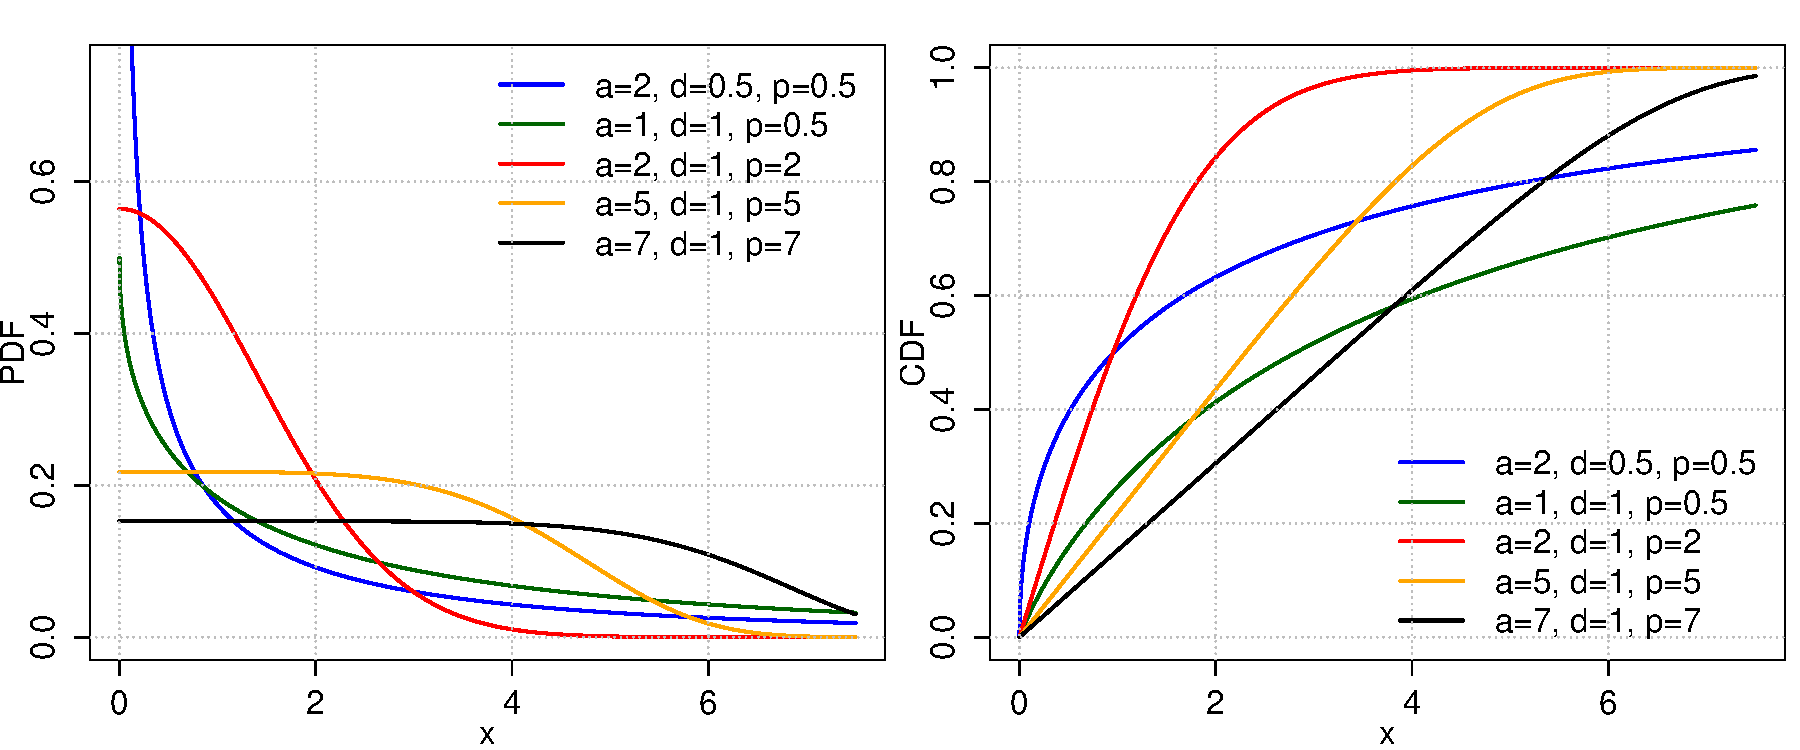
\includegraphics[width=140mm]{pics/GeneralisedGamma_pdf_cdf.pdf}
 \caption{PDF and CDF of the Generalised Gamma distribution plotted using the provided R-code.}
 \label{fig:GeneralisedGamma_pdf_cdf}
\end{figure}

\subsubsection*{Parameter: scale}

\noindent\begin{tabular}{p{2cm}cl}
\textbf{name} & & scale \\
\textbf{type} & & scalar \\
\textbf{symbol} & & $a$  \\
\textbf{definition} & & $a > 0$
\end{tabular}
\subsubsection*{Parameter: shape1}

\noindent\begin{tabular}{p{2cm}cl}
\textbf{name} & & shape \\
\textbf{type} & & scalar \\
\textbf{symbol} & & $d$  \\
\textbf{definition} & & $d > 0$
\end{tabular}
\subsubsection*{Parameter: shape2}

\noindent\begin{tabular}{p{2cm}cl}
\textbf{name} & & shape \\
\textbf{type} & & - \\
\textbf{symbol} & & $p$  \\
\textbf{definition} & & $p > 0$
\end{tabular}
\subsubsection*{Functions}

\smallskip \noindent \hspace{.2cm} \textbf{PDF} 
\begin{equation*}\frac{p/a^d}{\Gamma(d/p)} x^{d-1}e^{-(x/a)^p}\end{equation*}
\smallskip \noindent \hspace{.2cm} \textbf{PDF in R}  
\begin{verbatim}p/a^d/gamma(d/p) * x^(d-1) * exp(-(x/a)^p)\end{verbatim}
\smallskip \noindent \hspace{.2cm} \textbf{CDF} 
\begin{equation*}\frac{\gamma(d/p, (x/a)^p)}{\Gamma(d/p)}\end{equation*}
\smallskip \noindent \hspace{.2cm} \textbf{CDF in R} 
\begin{verbatim}Igamma(d/p, (x/a)^p, lower=T) / gamma(d/p)\end{verbatim}
%\smallskip\section*{GeneralizedGamma2} 
%
%  \bigskip 
%
%\begin{tabular}{p{2cm}cl}
%\textbf{name} & & Generalized Gamma 2 (ID: 0000148)\\ 
% 
%\textbf{type} & & continuous \\ 
%
%\textbf{variate} & & $x$, scalar \\ 
%
%\textbf{support} & & $0 < a < x$
%\end{tabular}
%\subsubsection*{Parameter: location}
%
%\noindent\begin{tabular}{p{2cm}cl}
%\textbf{name} & & location \\
%\textbf{type} & & scalar \\
%\textbf{symbol} & & $a$  \\
%\textbf{definition} & & $a > 0$
%\end{tabular}
%\subsubsection*{Parameter: scale}
%
%\noindent\begin{tabular}{p{2cm}cl}
%\textbf{name} & & b > 0 \\
%\textbf{type} & & scalar \\
%\textbf{symbol} & & $b$  \\
%\textbf{definition} & & $scale$
%\end{tabular}
%\subsubsection*{Parameter: shape1}
%
%\noindent\begin{tabular}{p{2cm}cl}
%\textbf{name} & & shape \\
%\textbf{type} & & scalar \\
%\textbf{symbol} & & $c$  \\
%\textbf{definition} & & $c > 0$
%\end{tabular}
%\subsubsection*{Parameter: shape2}
%
%\noindent\begin{tabular}{p{2cm}cl}
%\textbf{name} & & shape2 \\
%\textbf{type} & & scalar \\
%\textbf{symbol} & & $k$  \\
%\textbf{definition} & & $k > 0$
%\end{tabular}
%\subsubsection*{Functions}
%
%\smallskip \noindent \hspace{.2cm} \textbf{PDF} 
%\begin{equation*}\frac{k (x-a)^{kc-1}}{b^{kc}\Gamma(c)}\exp\Big[-\Big(\frac{x-a}{b}\Big)^k\Big]\end{equation*}
%\smallskip \noindent \hspace{.2cm} \textbf{CDF} 
%\begin{equation*}-\end{equation*}
\smallskip\section*{GeneralizedPoisson} 

  \bigskip 

\begin{tabular}{p{2cm}cl}
\textbf{name} & & Generalized Poisson (ID: 0000160)\\ 
 
\textbf{type} & & discrete \\ 

\textbf{variate} & & $k
$, scalar \\ 

\textbf{support} & & $k \in \{0,1,2,3,\dots\}$
\end{tabular}

\begin{figure}[ht!]
\centering
  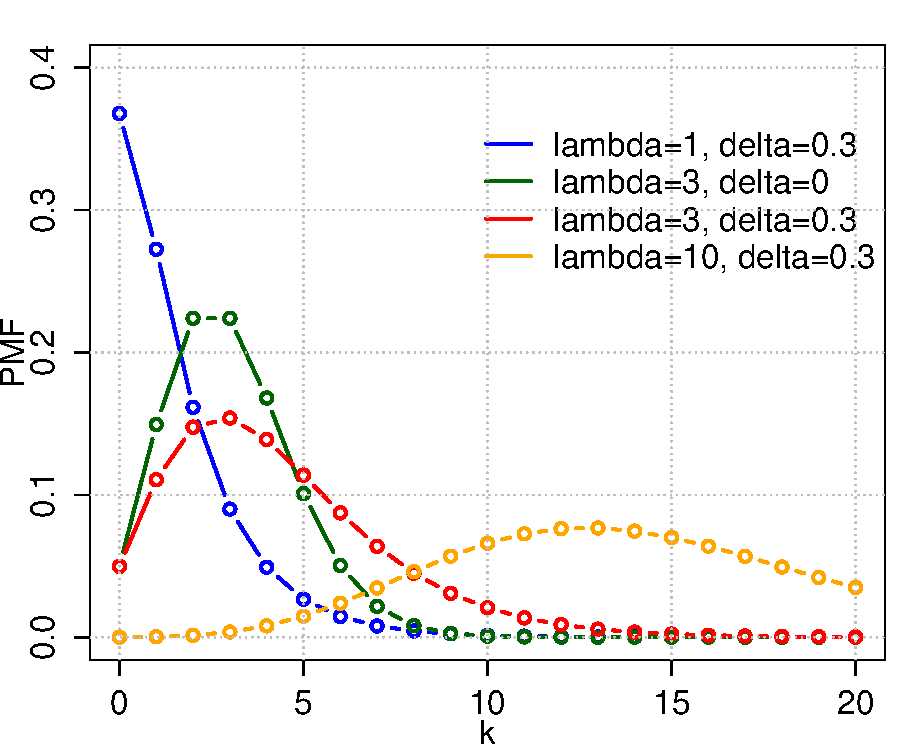
\includegraphics[width=70mm]{pics/GeneralisedPoisson_pmf_cdf.pdf}
 \caption{PMF of the Generalised Poisson distribution plotted using the provided R-code.}
 \label{fig:GeneralisedPoisson_pmf_cdf}
\end{figure}

\subsubsection*{Parameter: rate}

\noindent\begin{tabular}{p{2cm}cl}
\textbf{name} & & Poisson intensity \\
\textbf{type} & & scalar \\
\textbf{symbol} & & $\lambda$  \\
\textbf{definition} & & $\lambda \in R, \lambda > 0$
\end{tabular}
\subsubsection*{Parameter: dispersion}

\noindent\begin{tabular}{p{2cm}cl}
\textbf{name} & & dispersion \\
\textbf{type} & & scalar \\
\textbf{symbol} & & $\delta$  \\
\textbf{definition} & & $\max(-1,-\lambda/4) < \delta < 1$
\end{tabular}
\subsubsection*{Functions}

\smallskip \noindent \hspace{.2cm} \textbf{PMF} 
\begin{equation*}\frac{\lambda (\lambda+k\delta)^{k-1}\times e^{-\lambda - k \delta}}{k!}\end{equation*}
\smallskip \noindent \hspace{.2cm} \textbf{PMF in R}  
\begin{verbatim}(lambda*(lambda+k*delta)^(k-1) * exp(-lambda-k*delta)) / factorial(k)\end{verbatim}
\smallskip \noindent \hspace{.2cm} \textbf{CDF} 
\begin{equation*}-\end{equation*}
\smallskip\section*{Geometric} 

  \bigskip 

\begin{tabular}{p{2cm}cl}
\textbf{name} & & Geometric (ID: 0000128)\\ 
 
\textbf{type} & & discrete \\ 

\textbf{variate} & & $k
$, scalar \\ 

\textbf{support} & & $k \in \{0,1,2,3,\dots\}$
\end{tabular}

\begin{figure}[htb!]
\centering
  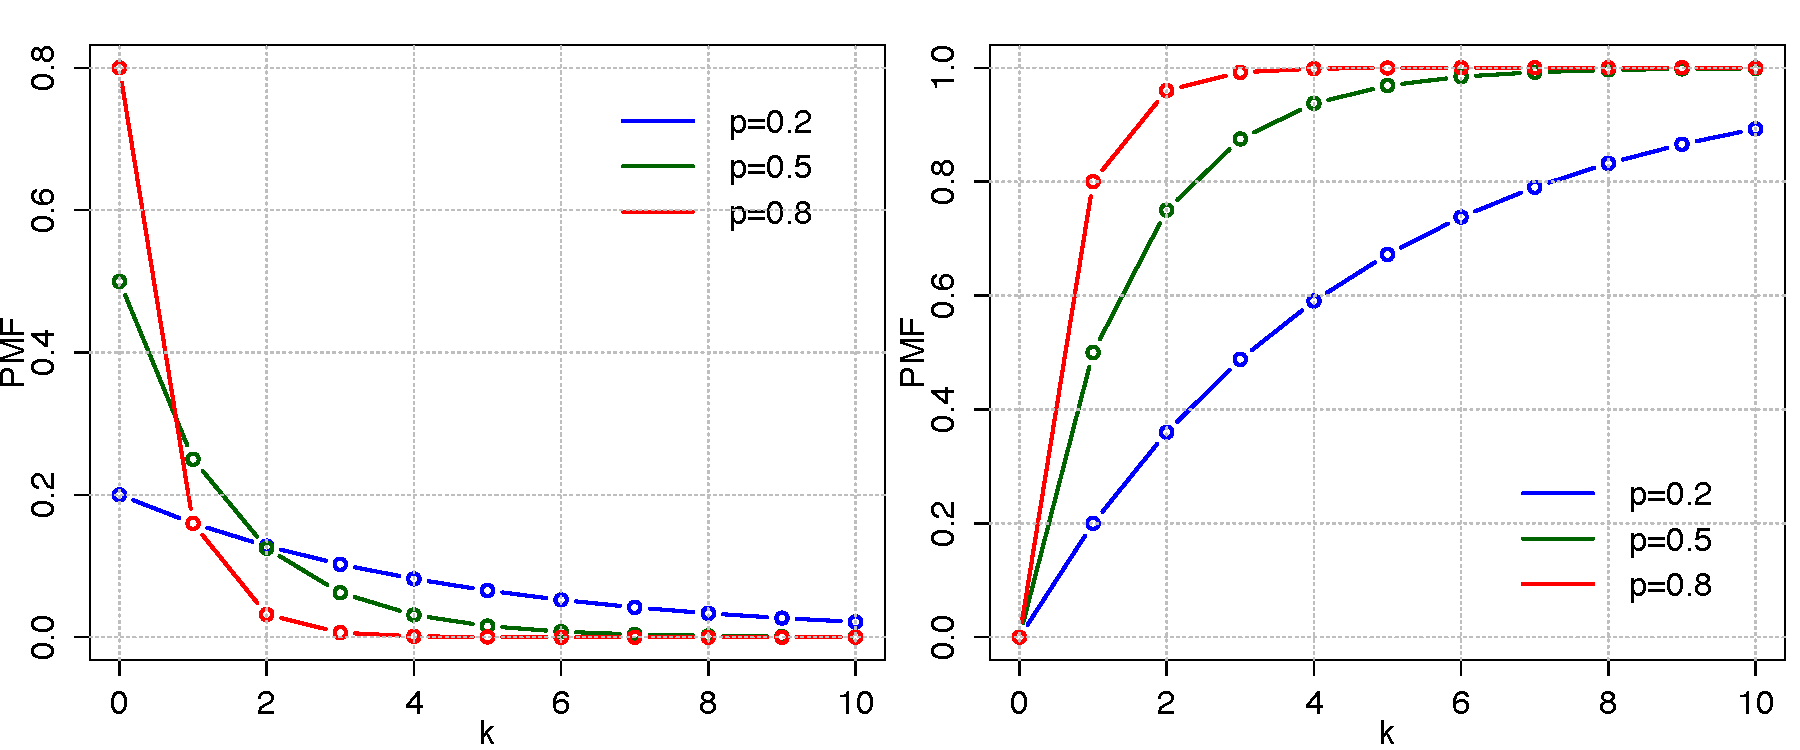
\includegraphics[width=140mm]{pics/Geometric_pmf_cdf.pdf}
 \caption{PMF and CDF of the Geometric distribution plotted using the provided R-code.}
 \label{fig:Geometric_pmf_cdf}
\end{figure}

\subsubsection*{Parameter: probability}

\noindent\begin{tabular}{p{2cm}cl}
\textbf{name} & & success probability \\
\textbf{type} & & scalar \\
\textbf{symbol} & & $p$  \\
\textbf{definition} & & $0< p \leq 1$
\end{tabular}
\subsubsection*{Functions}

\smallskip \noindent \hspace{.2cm} \textbf{PMF} 
\begin{equation*}(1 - p)^k\,p\end{equation*}
\smallskip \noindent \hspace{.2cm} \textbf{PMF in R}  
\begin{verbatim}p*(1-p)^k\end{verbatim}
\smallskip \noindent \hspace{.2cm} \textbf{CDF} 
\begin{equation*}1-(1 - p)^{k+1}\end{equation*}
\smallskip \noindent \hspace{.2cm} \textbf{CDF in R} 
\begin{verbatim}1-(1 - p)^(k+1)\end{verbatim}
\smallskip\section*{Gompertz} 

  \bigskip 

\begin{tabular}{p{2cm}cl}
\textbf{name} & & Gompertz (ID: 0000172)\\ 
 
\textbf{type} & & continuous \\ 

\textbf{variate} & & $x$, scalar \\ 

\textbf{support} & & $x \in (-\infty,+\infty)$
\end{tabular}

\begin{figure}[ht!]
\centering
  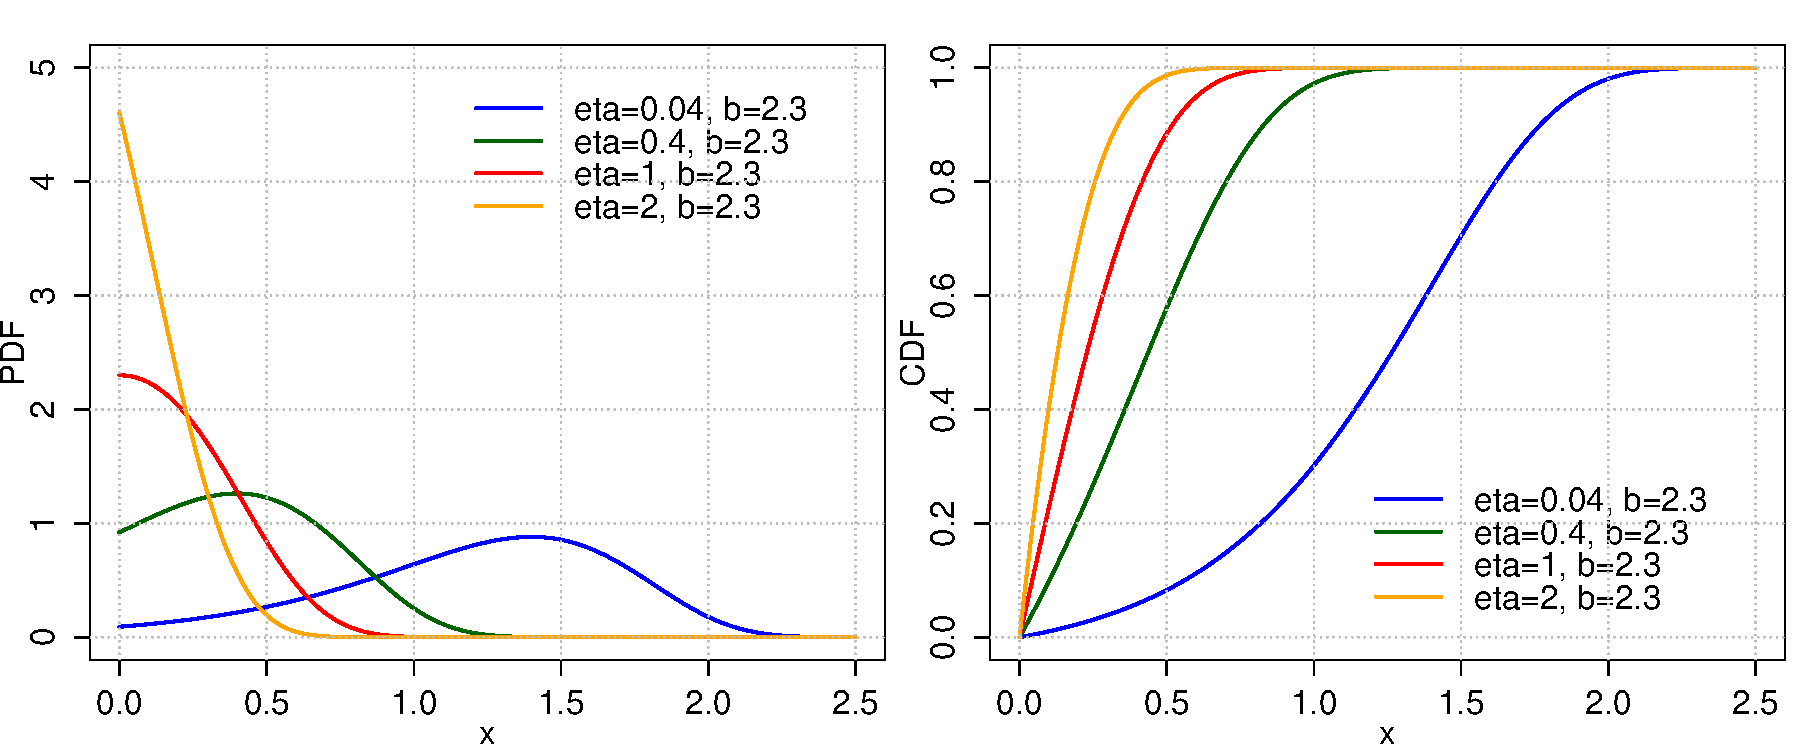
\includegraphics[width=140mm]{pics/Gompertz_pdf_cdf.pdf}
 \caption{PMF of the Gompertz distribution plotted using the provided R-code.}
 \label{fig:Gompertz_pdf_cdf}
\end{figure}

\subsubsection*{Parameter: shape}

\noindent\begin{tabular}{p{2cm}cl}
\textbf{name} & & shape \\
\textbf{type} & & scalar \\
\textbf{symbol} & & $\eta$  \\
\textbf{definition} & & $\eta > 0$
\end{tabular}
\subsubsection*{Parameter: scale}

\noindent\begin{tabular}{p{2cm}cl}
\textbf{name} & & scale \\
\textbf{type} & & scalar \\
\textbf{symbol} & & $b$  \\
\textbf{definition} & & $b > 0$
\end{tabular}
\subsubsection*{Functions}

\smallskip \noindent \hspace{.2cm} \textbf{PDF} 
\begin{equation*}b\eta e^{bx}e^{\eta}\exp\left(-\eta e^{bx} \right)\end{equation*}
\smallskip \noindent \hspace{.2cm} \textbf{PDF in R}  
\begin{verbatim}b*eta*exp(b*x)*exp(eta)*exp(-eta*exp(b*x))\end{verbatim}
\smallskip \noindent \hspace{.2cm} \textbf{CDF} 
\begin{equation*}1-\exp\left(-\eta\left(e^{bx}-1 \right)\right)\end{equation*}
\smallskip \noindent \hspace{.2cm} \textbf{CDF in R} 
\begin{verbatim}1-exp(-eta*(exp(b*x)-1))\end{verbatim}
\smallskip\section*{Gumbel} 

  \bigskip 

\begin{tabular}{p{2cm}cl}
\textbf{name} & & Gumbel (ID: 0000182)\\ 
 
\textbf{type} & & continuous \\ 

\textbf{variate} & & $x$, scalar \\ 

\textbf{support} & & $x \in (-\infty,+\infty)$
\end{tabular}

\begin{figure}[htb!]
\centering
  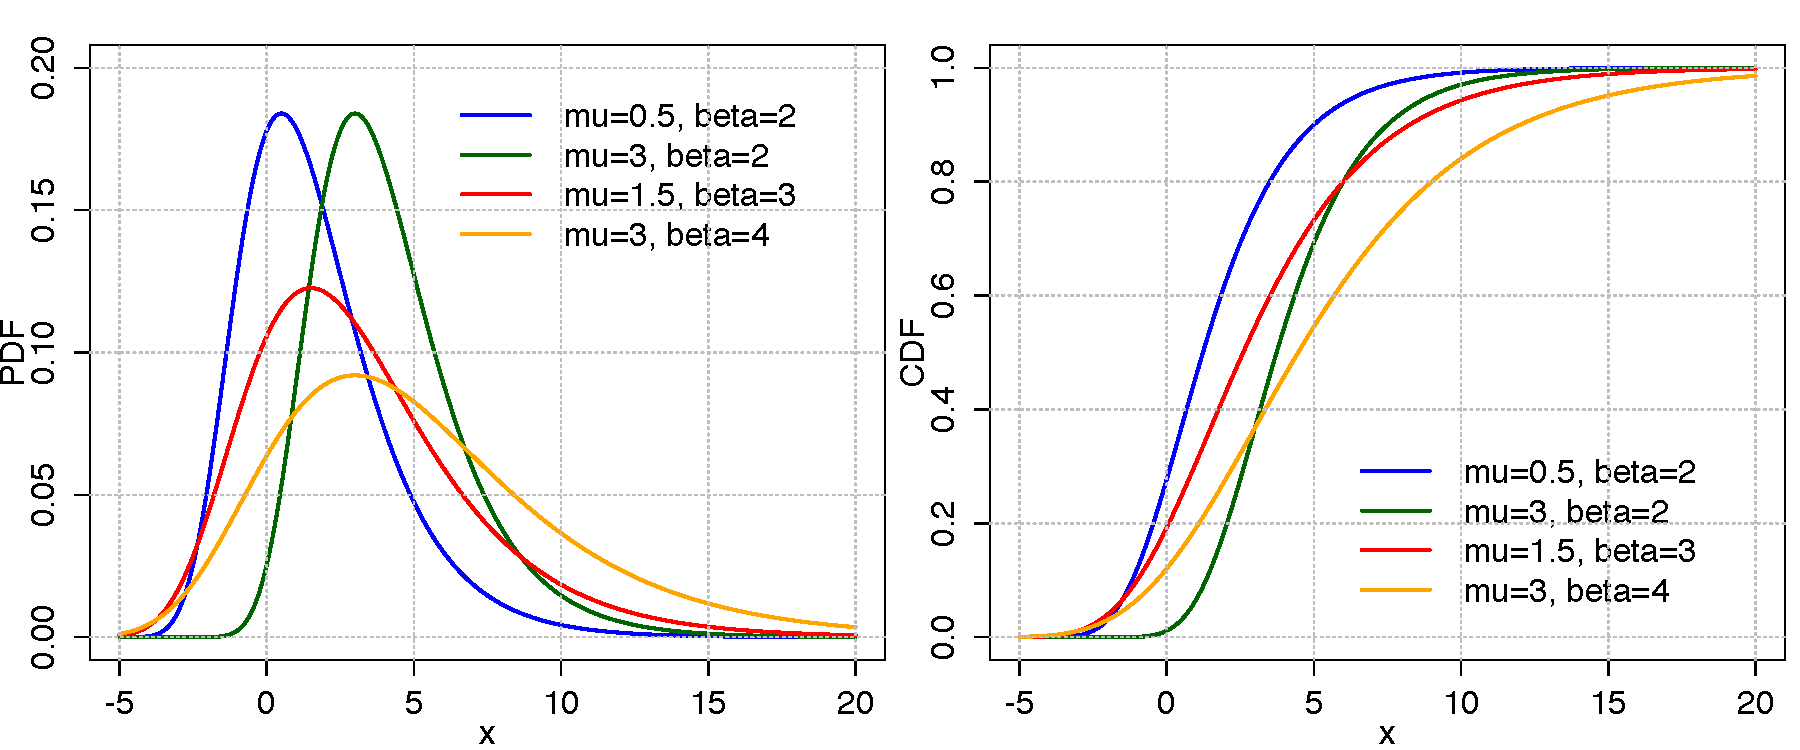
\includegraphics[width=140mm]{pics/Gumbel_pdf_cdf.pdf}
 \caption{PDF of the Gumbel distribution plotted using the provided R-code.}
 \label{fig:Gumbel_pdf_cdf}
\end{figure}

\subsubsection*{Parameter: location}

\noindent\begin{tabular}{p{2cm}cl}
\textbf{name} & & location \\
\textbf{type} & & scalar \\
\textbf{symbol} & & $\mu$  \\
\textbf{definition} & & $\mu \in  R$
\end{tabular}
\subsubsection*{Parameter: scale}

\noindent\begin{tabular}{p{2cm}cl}
\textbf{name} & & scale \\
\textbf{type} & & scalar \\
\textbf{symbol} & & $\beta$  \\
\textbf{definition} & & $\beta>0, \beta \in  R$
\end{tabular}
\subsubsection*{Functions}

\smallskip \noindent \hspace{.2cm} \textbf{PDF} 
\begin{equation*}\frac{e^{-e^{-\frac{x-\mu}{\beta}}} e^{-\frac{x-\mu}{\beta}}}{\beta}\end{equation*}
\smallskip \noindent \hspace{.2cm} \textbf{CDF} 
\begin{equation*}e^{-e^{-(x-\mu)/\beta}}\end{equation*}
\smallskip\section*{Hypergeometric} 

  \bigskip 

\begin{tabular}{p{2cm}cl}
\textbf{name} & & Hypergeometric (ID: 0000191)\\ 
 
\textbf{type} & & discrete \\ 

\textbf{variate} & & $k
$, scalar \\ 

\textbf{support} & & $k\, \in\, \left\{\max{(0,\, n+K-N)},\, \dots,\, \min{(n,\, K )}\right\}$
\end{tabular}

\begin{figure}[htb!]
\centering
  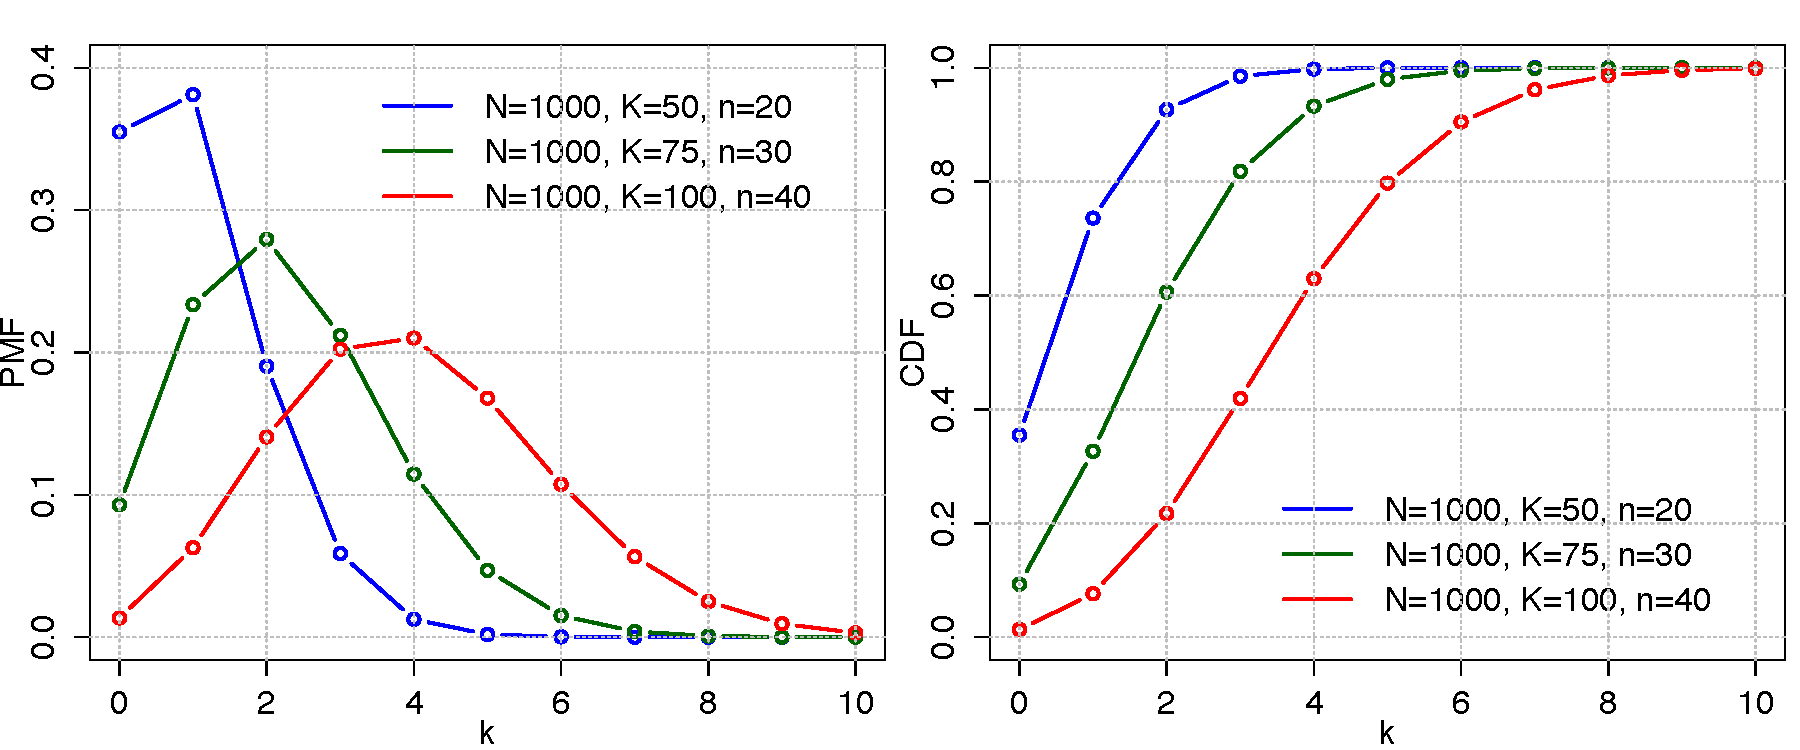
\includegraphics[width=140mm]{pics/Hypergeometric_pmf_cdf.pdf}
 \caption{PMF and CDF of the Hypergeometric distribution plotted using the provided R-code.}
 \label{fig:Hypergeometric_pmf_cdf}
\end{figure}

\subsubsection*{Parameter: populationSize}

\noindent\begin{tabular}{p{2cm}cl}
\textbf{name} & & population size \\
\textbf{type} & & scalar \\
\textbf{symbol} & & $N$  \\
\textbf{definition} & & $N \in \left\{0,1,2,\dots\right\}$
\end{tabular}
\subsubsection*{Parameter: numberOfTrials}

\noindent\begin{tabular}{p{2cm}cl}
\textbf{name} & & number of trials \\
\textbf{type} & & scalar \\
\textbf{symbol} & & $K$  \\
\textbf{definition} & & $K \in \left\{0,1,2,\dots,N\right\} $
\end{tabular}
\subsubsection*{Parameter: numberOfSuccesses}

\noindent\begin{tabular}{p{2cm}cl}
\textbf{name} & & number of successes \\
\textbf{type} & & scalar \\
\textbf{symbol} & & $n$  \\
\textbf{definition} & & $n \in \left\{0,1,2,\dots,N\right\}$
\end{tabular}
\subsubsection*{Functions}

\smallskip \noindent \hspace{.2cm} \textbf{PMF} 
\begin{equation*}{{{K \choose k} {{N-K} \choose {n-k}}}\over {N \choose n}}\end{equation*}
\smallskip \noindent \hspace{.2cm} \textbf{PMF in R}  
\begin{verbatim}choose(K,k)*choose(M-K,n-k)/choose(M,n)\end{verbatim}
\smallskip \noindent \hspace{.2cm} \textbf{CDF} 
\begin{equation*}1-{{{n \choose {k+1}}{{N-n} \choose {K-k-1}}}\over {N \choose K}} \,_3F_2\!\!\left[\begin{array}{c}1,\ k+1-K,\ k+1-n \\ k+2,\ N+k+2-K-n\end{array};1\right]\end{equation*}
\smallskip \noindent \hspace{.2cm} \textbf{CDF in R} 
\begin{verbatim}cumsum(PMF)\end{verbatim}
\smallskip\section*{InverseGamma} 

  \bigskip 

\begin{tabular}{p{2cm}cl}
\textbf{name} & & Inverse-Gamma (ID: 0000201)\\ 
 
\textbf{type} & & continuous \\ 

\textbf{variate} & & $x$, scalar \\ 

\textbf{support} & & $x \in (0,+\infty)$
\end{tabular}

%%%%%%%%%%%%%%%%%%%%%%%%%%%%%%%%%
\begin{figure}[htb!]
\centering
  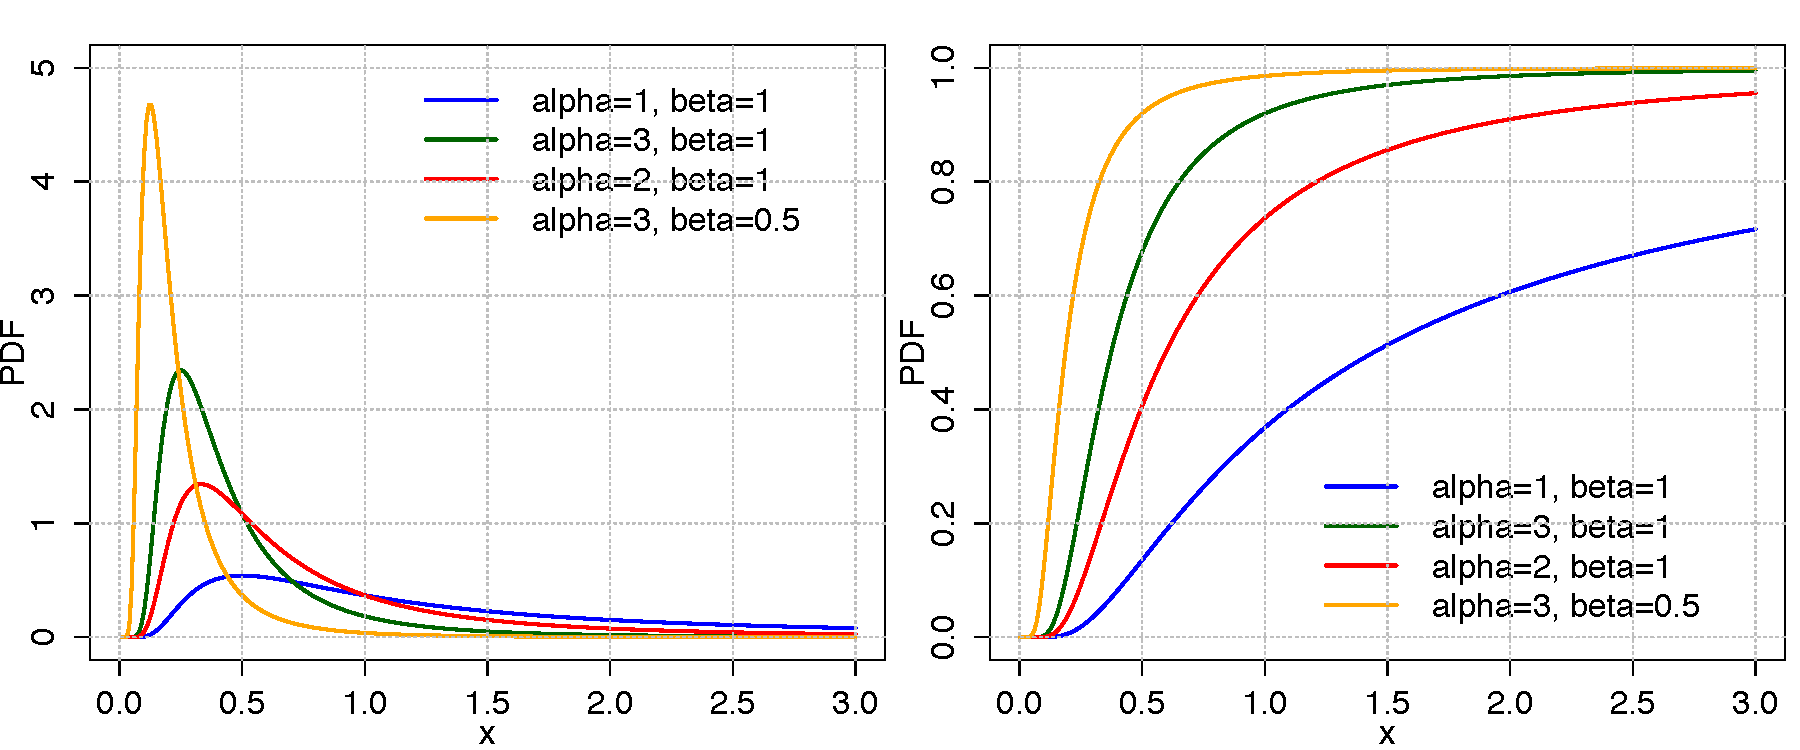
\includegraphics[width=140mm]{pics/InverseGamma_pdf_cdf.pdf}
 \caption{PDF of the Inverse Gamma distribution plotted using the provided R-code.}
 \label{fig:InverseGamma_pdf_cdf}
\end{figure}

\subsubsection*{Parameter: shape}

\noindent\begin{tabular}{p{2cm}cl}
\textbf{name} & & shape \\
\textbf{type} & & scalar \\
\textbf{symbol} & & $\alpha$  \\
\textbf{definition} & & $\alpha>0, \alpha \in  R$
\end{tabular}
\subsubsection*{Parameter: scale}

\noindent\begin{tabular}{p{2cm}cl}
\textbf{name} & & scale \\
\textbf{type} & & scalar \\
\textbf{symbol} & & $\beta$  \\
\textbf{definition} & & $\beta>0, \beta \in  R$
\end{tabular}
\subsubsection*{Functions}

\smallskip \noindent \hspace{.2cm} \textbf{PDF} 
\begin{equation*}\frac{\beta^\alpha}{\Gamma(\alpha)} x^{-\alpha - 1} \exp \left(\frac{-\beta}{x}\right)\end{equation*}
\smallskip \noindent \hspace{.2cm} \textbf{CDF} 
\begin{equation*}\frac{\Gamma(\alpha, \beta/x)}{\Gamma(\alpha)}\end{equation*}
\smallskip\section*{InverseGaussian} 

  \bigskip 

\begin{tabular}{p{2cm}cl}
\textbf{name} & & Inverse Gaussian (ID: 0000211)\\ 
 
\textbf{type} & & continuous \\ 

\textbf{variate} & & $$,  \\ 

\textbf{support} & & $$
\end{tabular}

\begin{figure}[htb!]
\centering
  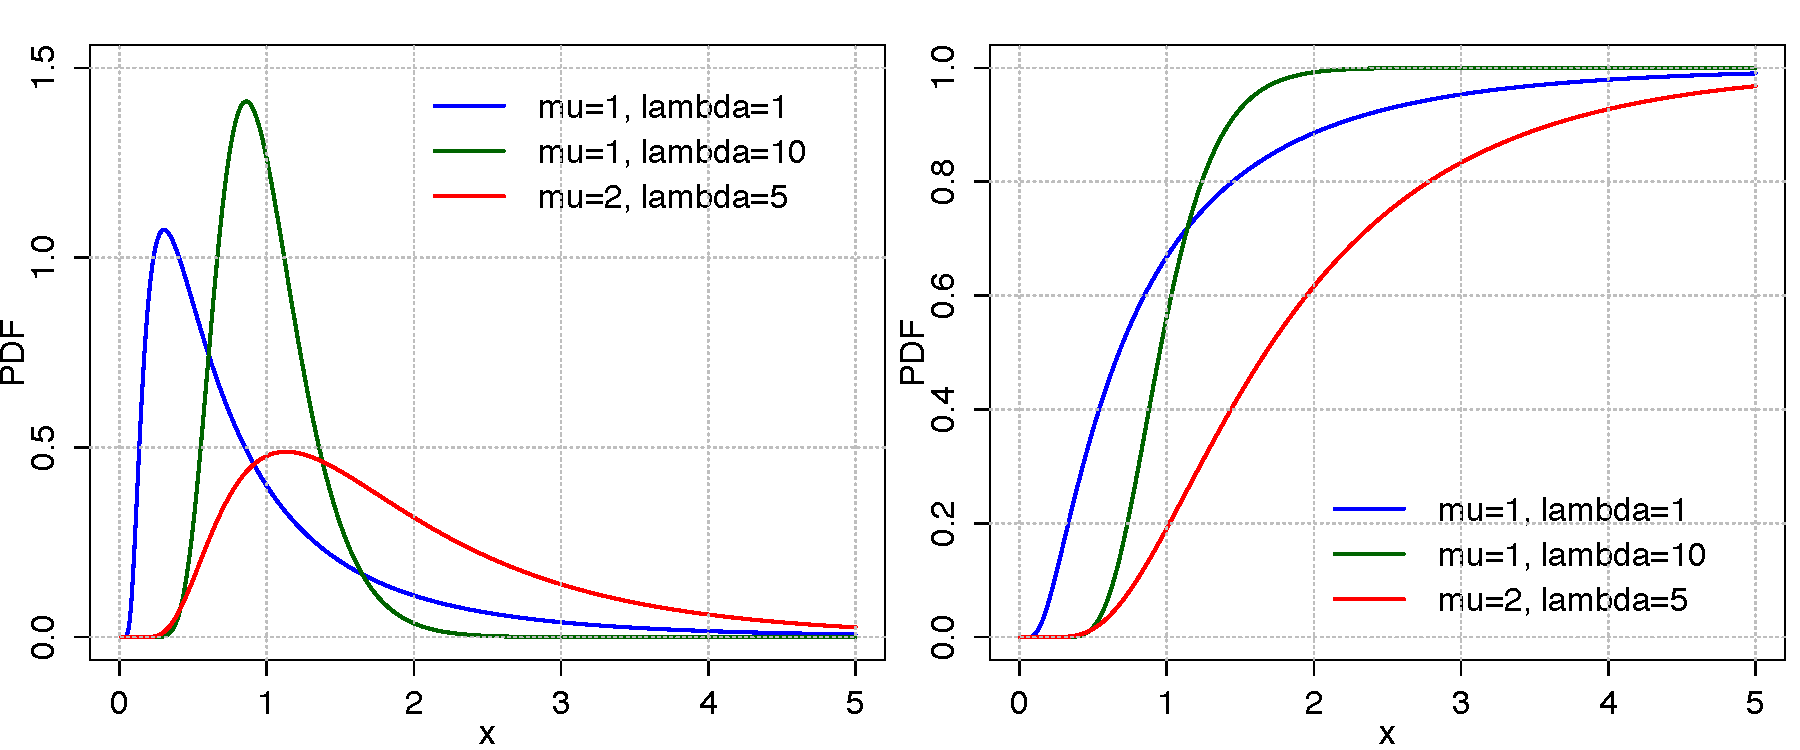
\includegraphics[width=140mm]{pics/InverseGaussian_pdf_cdf.pdf}
 \caption{PDF of the Inverse Gaussian distribution plotted using the provided R-code.}
 \label{fig:InverseGaussian_pdf_cdf}
\end{figure}

\subsubsection*{Parameter: shape}

\noindent\begin{tabular}{p{2cm}cl}
\textbf{name} & & shape \\
\textbf{type} & & scalar \\
\textbf{symbol} & & $\lambda$  \\
\textbf{definition} & & $\lambda > 0$
\end{tabular}
\subsubsection*{Parameter: mean}

\noindent\begin{tabular}{p{2cm}cl}
\textbf{name} & & mean \\
\textbf{type} & & scalar \\
\textbf{symbol} & & $\mu$  \\
\textbf{definition} & & $\mu > 0$
\end{tabular}
\subsubsection*{Functions}

\smallskip \noindent \hspace{.2cm} \textbf{PDF} 
\begin{equation*}\sqrt{\frac{\lambda}{2\pi x^3}} \exp\Big(-\frac{\lambda}{2\mu^2 x}(x-\mu)^2\Big)\end{equation*}
\smallskip \noindent \hspace{.2cm} \textbf{PDF in R}  
\begin{verbatim}sqrt(lambda/(2*pi*x^3) ) * exp(-lambda/(2*mu^2 x) * (x-mu)^2)\end{verbatim}
\smallskip \noindent \hspace{.2cm} \textbf{CDF} 
\begin{equation*}\Phi\left(\sqrt{\frac{\lambda}{x}} \left(\frac{x}{\mu}-1 \right)\right) +\exp\left(\frac{2 \lambda}{\mu}\right) \Phi\left(-\sqrt{\frac{\lambda}{x}}\left(\frac{x}{\mu}+1 \right)\right)\end{equation*}
\smallskip \noindent \hspace{.2cm} \textbf{CDF in R} 
\begin{verbatim}pnorm(sqrt(lambda/x) * (x/mu-1)) + exp(2*lambda/mu) * pnorm(-sqrt(lambda/x) * (x/mu+1))\end{verbatim}
\smallskip\section*{InverseWishart} 

  \bigskip 

\begin{tabular}{p{2cm}cl}
\textbf{name} & & Inverse-Wishart (ID: 0000220)\\ 
 
\textbf{type} & & continuous \\ 

\textbf{variate} & & $X$, matrix \\ 

\textbf{support} & & $X(p \times p) - \text{positive-definite matrix}$
\end{tabular}
\subsubsection*{Parameter: scaleMatrix}

\noindent\begin{tabular}{p{2cm}cl}
\textbf{name} & & scale matrix \\
\textbf{type} & & matrix \\
\textbf{symbol} & & $\Psi$  \\
\textbf{definition} & & $\Psi > 0, \text{positive-definite matrix}$
\end{tabular}
\subsubsection*{Parameter: degreesOfFreedom}

\noindent\begin{tabular}{p{2cm}cl}
\textbf{name} & & degrees of freedom \\
\textbf{type} & & scalar \\
\textbf{symbol} & & $\nu$  \\
\textbf{definition} & & $\nu > p-1, \nu \in  R$
\end{tabular}
\subsubsection*{Functions}

\smallskip \noindent \hspace{.2cm} \textbf{PDF} 
\begin{equation*}\frac{\left|\Psi\right|^{\frac{\nu}{2}}}{2^{\frac{\nu p}{2}}\Gamma_p(\frac{\nu}{2})} \left|X\right|^{-\frac{\nu+p+1}{2}}e^{-\frac{1}{2}\text{tr}(\Psi X^{-1})}\end{equation*}
\smallskip \noindent \hspace{.2cm} \textbf{CDF} 
\begin{equation*}-\end{equation*}
\smallskip\section*{Laplace1} 

  \bigskip 

\begin{tabular}{p{2cm}cl}
\textbf{name} & & Laplace 1 (ID: 0000230)\\ 
 
\textbf{type} & & continuous \\ 

\textbf{variate} & & $x$, scalar \\ 

\textbf{support} & & $x \in (-\infty,+\infty)$
\end{tabular}

\begin{figure}[ht!]
\centering
  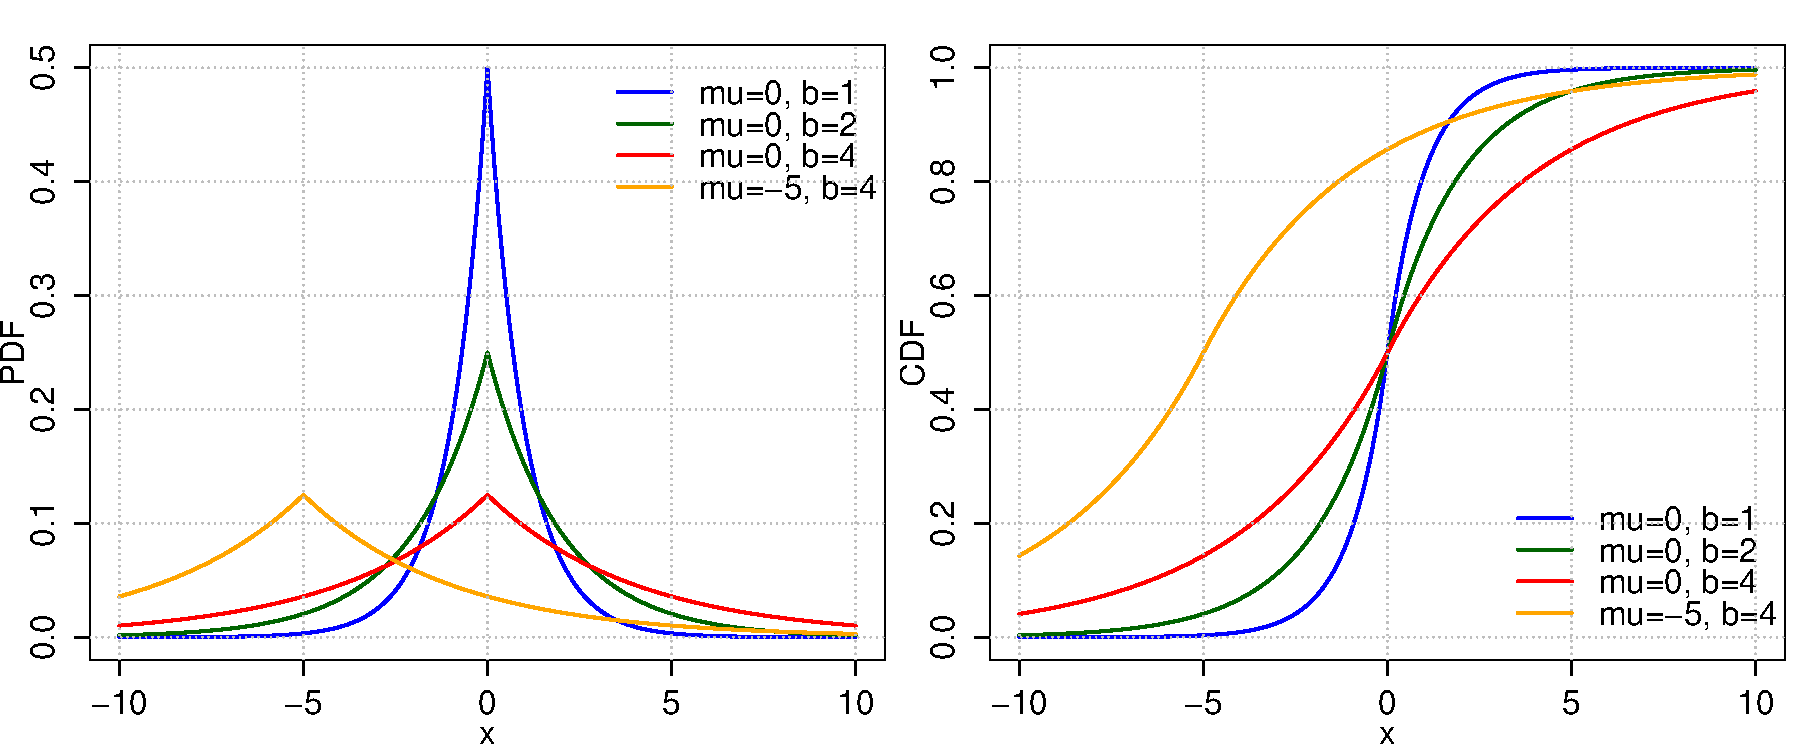
\includegraphics[width=140mm]{pics/Laplace1_pdf_cdf.pdf}
 \caption{PMF of the Laplace1 distribution plotted using the provided R-code.}
 \label{fig:Laplace1_pdf_cdf}
\end{figure}

\subsubsection*{Parameter: location}

\noindent\begin{tabular}{p{2cm}cl}
\textbf{name} & & location \\
\textbf{type} & & scalar \\
\textbf{symbol} & & $\mu$  \\
\textbf{definition} & & $\mu \in R$
\end{tabular}
\subsubsection*{Parameter: scale}

\noindent\begin{tabular}{p{2cm}cl}
\textbf{name} & & scale \\
\textbf{type} & & scalar \\
\textbf{symbol} & & $b$  \\
\textbf{definition} & & $b > 0, b \in R$
\end{tabular}
\subsubsection*{Functions}

\smallskip \noindent \hspace{.2cm} \textbf{PDF} 
\begin{equation*}\frac{1}{2\,b} \exp \left(-\frac{|x-\mu|}b \right)\end{equation*}
\smallskip \noindent \hspace{.2cm} \textbf{PDF in R}  
\begin{verbatim}1/(2*b) * exp(- abs(x-mu)/b )\end{verbatim}
\smallskip \noindent \hspace{.2cm} \textbf{CDF} 
\begin{equation*}\begin{cases}
      \frac12 \exp \left( \frac{x-\mu}{b} \right) & \mbox{if }x < \mu \\
          1-\frac12 \exp \left( -\frac{x-\mu}{b} \right) & \mbox{if }x \geq \mu
       \end{cases}\end{equation*}
\smallskip \noindent \hspace{.2cm} \textbf{CDF in R} 
\begin{verbatim}1/2 * exp( (x-mu)/b ) for x < mu
1- 1/2 * exp( -(x-mu)/b ) x >= mu\end{verbatim}
\smallskip\section*{Laplace2} 

  \bigskip 

\begin{tabular}{p{2cm}cl}
\textbf{name} & & Laplace 2 (ID: 0000241)\\ 
 
\textbf{type} & & continuous \\ 

\textbf{variate} & & $x$, scalar \\ 

\textbf{support} & & $x \in (-\infty,+\infty)$
\end{tabular}
\subsubsection*{Parameter: location}

\noindent\begin{tabular}{p{2cm}cl}
\textbf{name} & & - \\
\textbf{type} & & scalar \\
\textbf{symbol} & & $\mu$  \\
\textbf{definition} & & $-$
\end{tabular}
\subsubsection*{Parameter: tau}

\noindent\begin{tabular}{p{2cm}cl}
\textbf{name} & & - \\
\textbf{type} & & scalar \\
\textbf{symbol} & & $\tau$  \\
\textbf{definition} & & $-$
\end{tabular}
\subsubsection*{Functions}

\smallskip \noindent \hspace{.2cm} \textbf{PDF} 
\begin{equation*}\frac{\tau}{2} \exp \left(-\tau|x-\mu| \right)\end{equation*}
\smallskip \noindent \hspace{.2cm} \textbf{CDF} 
\begin{equation*}-\end{equation*}
\smallskip\section*{LogLogistic} 

  \bigskip 

\begin{tabular}{p{2cm}cl}
\textbf{name} & & Log-Logistic (ID: 0000263)\\ 
 
\textbf{type} & & continuous \\ 

\textbf{variate} & & $x$, scalar \\ 

\textbf{support} & & $x \in [0,+\infty)$
\end{tabular}

\begin{figure}[htb!]
\centering
  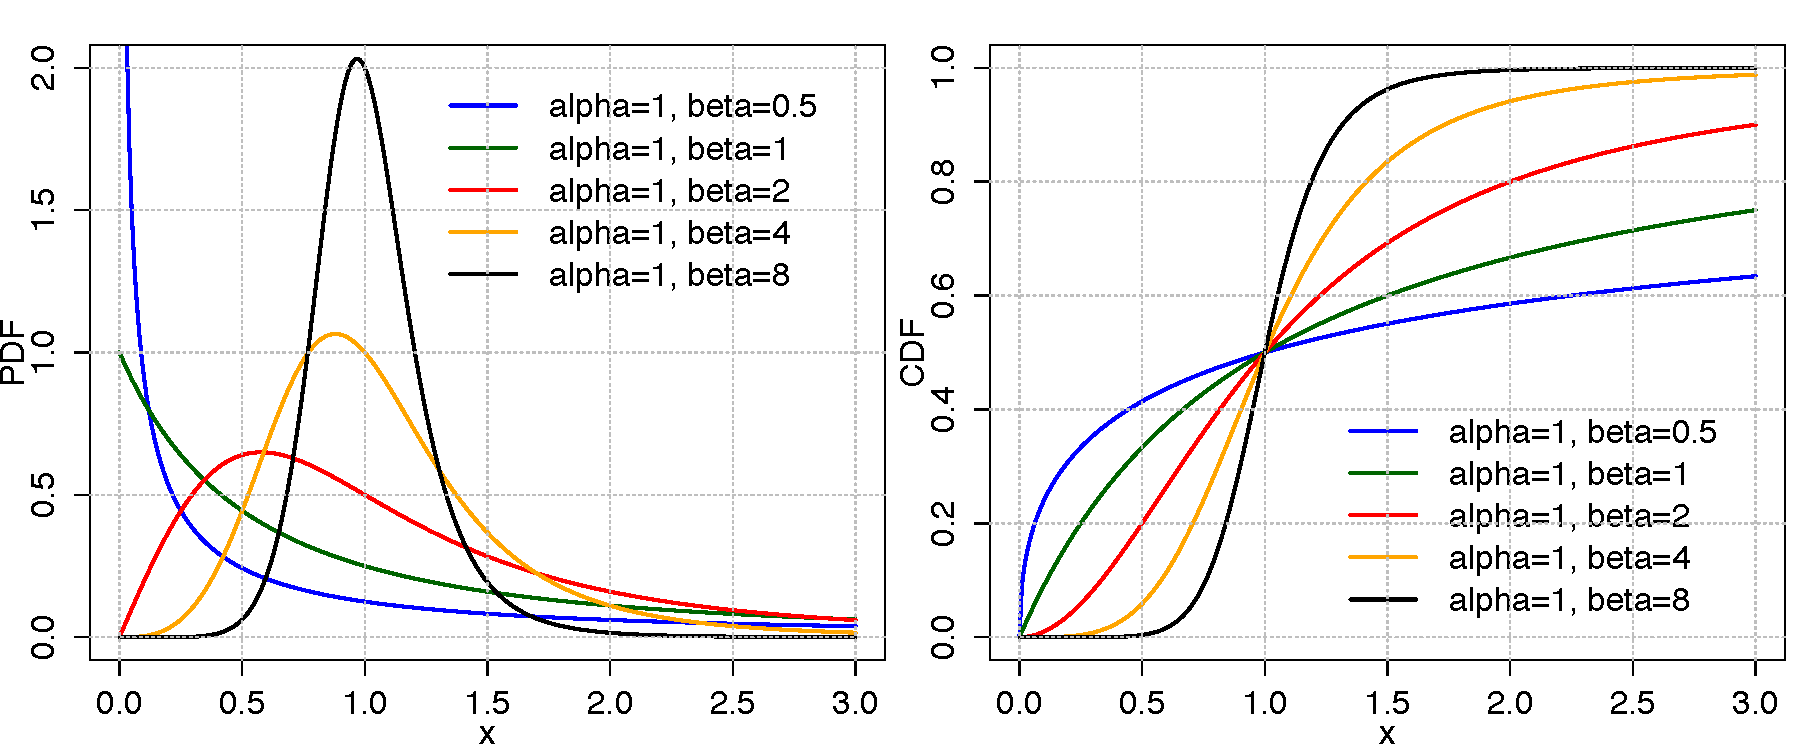
\includegraphics[width=140mm]{pics/LogLogistic_pdf_cdf.pdf}
 \caption{PDF and CDF of the Log-logistic distribution plotted using the provided R-code.}
 \label{fig:LogLogistic_pdf_cdf}
\end{figure}

\subsubsection*{Parameter: scale}

\noindent\begin{tabular}{p{2cm}cl}
\textbf{name} & & scale \\
\textbf{type} & & scalar \\
\textbf{symbol} & & $\alpha$  \\
\textbf{definition} & & $\alpha > 0$
\end{tabular}
\subsubsection*{Parameter: shape}

\noindent\begin{tabular}{p{2cm}cl}
\textbf{name} & & shape \\
\textbf{type} & & scalar \\
\textbf{symbol} & & $\beta$  \\
\textbf{definition} & & $\beta > 0$
\end{tabular}
\subsubsection*{Functions}

\smallskip \noindent \hspace{.2cm} \textbf{PDF} 
\begin{equation*}\frac{(\beta/\alpha)(x/\alpha)^{\beta-1}}{(1+(x/\alpha)^\beta)^2}\end{equation*}
\smallskip \noindent \hspace{.2cm} \textbf{PDF in R}  
\begin{verbatim}(beta/alpha)*(x/alpha)^(beta-1) / (1+(x/alpha)^beta)^2\end{verbatim}
\smallskip \noindent \hspace{.2cm} \textbf{CDF} 
\begin{equation*}\frac{1}{1+(x/\alpha)^{-\beta}}\end{equation*}
\smallskip \noindent \hspace{.2cm} \textbf{CDF in R} 
\begin{verbatim}1 / (1+(x/alpha)^(-beta))\end{verbatim}
\smallskip\section*{LogNormal1} 

  \bigskip 

\begin{tabular}{p{2cm}cl}
\textbf{name} & & Log-Normal 1 (ID: 0000274)\\ 
 
\textbf{type} & & continuous \\ 

\textbf{variate} & & $x$, scalar \\ 

\textbf{support} & & $x \in (0,+\infty)$
\end{tabular}
\subsubsection*{Parameter: meanLog}

\noindent\begin{tabular}{p{2cm}cl}
\textbf{name} & & mean of log(x) \\
\textbf{type} & & scalar \\
\textbf{symbol} & & $\mu$  \\
\textbf{definition} & & $\mu \in R$
\end{tabular}

\begin{figure}[htb!]
\centering
  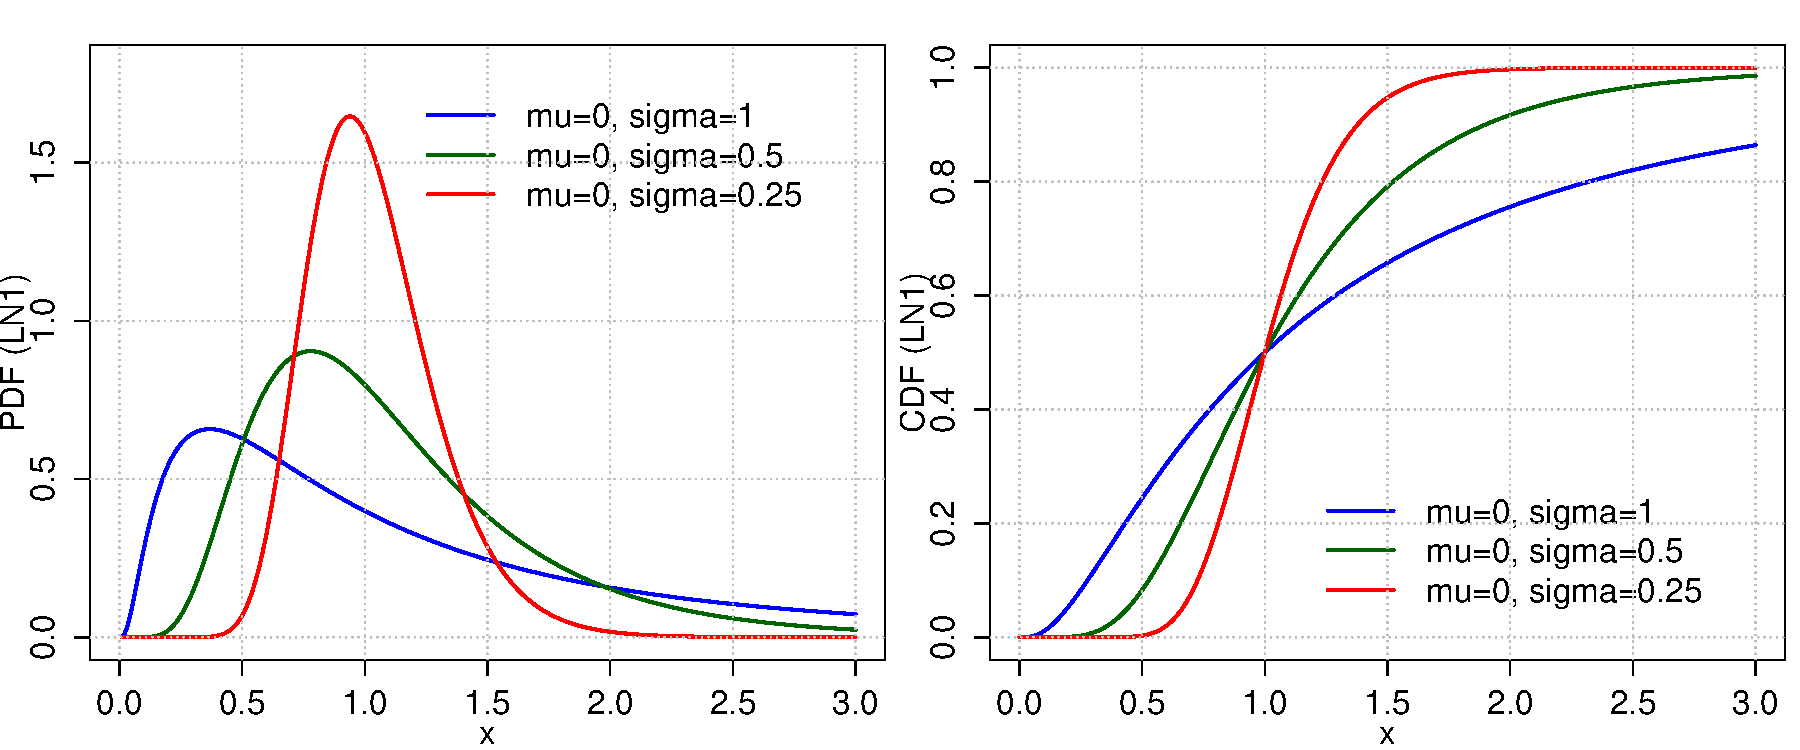
\includegraphics[width=140mm]{pics/LogNormal_pdf_cdf.pdf}
 \caption{PDF and CDF of the Log-Normal distribution, LN1,
 plotted using the provided R-code.}
 \label{fig:LN1pdfcdf}
\end{figure}

\subsubsection*{Parameter: stdevLog}

\noindent\begin{tabular}{p{2cm}cl}
\textbf{name} & & shape \\
\textbf{type} & & scalar \\
\textbf{symbol} & & $\sigma$  \\
\textbf{definition} & & $\sigma > 0$
\end{tabular}
\subsubsection*{Functions}

\smallskip \noindent \hspace{.2cm} \textbf{PDF} 
\begin{equation*}\frac{1}{x\sigma\sqrt{2\pi}}\ e^{-\frac{\left(\ln x-\mu\right)^2}{2\sigma^2}}\end{equation*}
\smallskip \noindent \hspace{.2cm} \textbf{PDF in R}  
\begin{verbatim}1/(x*sigma*sqrt(2*pi)) * exp((-(log(x)-mu)^2)/(2*sigma^2))\end{verbatim}
\smallskip \noindent \hspace{.2cm} \textbf{CDF} 
\begin{equation*}\frac12 + \frac12\,\text{erf}\Big[\frac{\ln x-\mu}{\sqrt{2}\sigma}\Big]\end{equation*}
\smallskip \noindent \hspace{.2cm} \textbf{CDF in R} 
\begin{verbatim}1/2 + 1/2 *erf( (log(x)-mu)/(sqrt(2)*sigma) )\end{verbatim}
\smallskip\section*{LogNormal2} 

  \bigskip 

\begin{tabular}{p{2cm}cl}
\textbf{name} & & Log-Normal 2 (ID: 0000284)\\ 
 
\textbf{type} & & continuous \\ 

\textbf{variate} & & $x$, scalar \\ 

\textbf{support} & & $x \in (0,+\infty)$
\end{tabular}

\begin{figure}[htb!]
\centering
  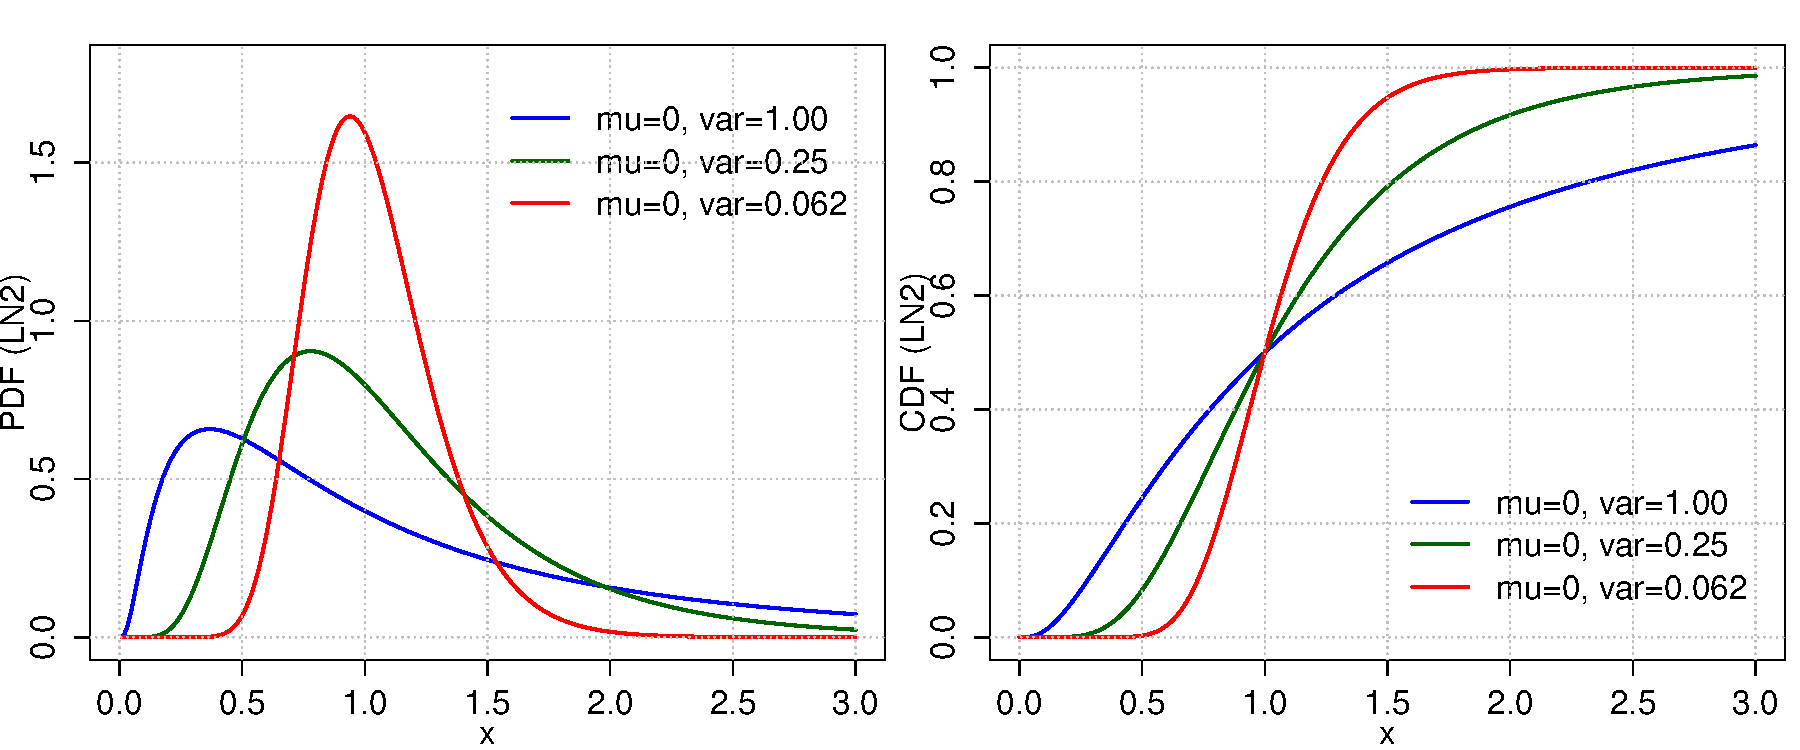
\includegraphics[width=140mm]{pics/LogNormal2_pdf_cdf.pdf}
 \caption{PDF and CDF of the Log-Normal distribution, LN1,
 plotted using the provided R-code.}
 \label{fig:LN2pdfcdf}
\end{figure}

\subsubsection*{Parameter: meanLog}

\noindent\begin{tabular}{p{2cm}cl}
\textbf{name} & & mean of log(x) \\
\textbf{type} & & scalar \\
\textbf{symbol} & & $\mu$  \\
\textbf{definition} & & $\mu \in R$
\end{tabular}
\subsubsection*{Parameter: varLog}

\noindent\begin{tabular}{p{2cm}cl}
\textbf{name} & & shape \\
\textbf{type} & & scalar \\
\textbf{symbol} & & $v$  \\
\textbf{definition} & & $v > 0$
\end{tabular}
\subsubsection*{Functions}

\smallskip \noindent \hspace{.2cm} \textbf{PDF} 
\begin{equation*}\frac{1}{x\sqrt{v}\sqrt{2\pi}}\ e^{-\frac{\left(\ln x-\mu\right)^2}{2 v}}\end{equation*}
\smallskip \noindent \hspace{.2cm} \textbf{PDF in R}  
\begin{verbatim}1/(x*sqrt(v)*sqrt(2*pi)) * exp(-(ln(x)-mu)^2/(2*v))\end{verbatim}
\smallskip \noindent \hspace{.2cm} \textbf{CDF} 
\begin{equation*}\frac12 + \frac12\,\text{erf}\Big[\frac{\ln x-\mu}{\sqrt{2}\sqrt{var}}\Big]\end{equation*}
\smallskip \noindent \hspace{.2cm} \textbf{CDF in R} 
\begin{verbatim}1/2 + 1/2 * erf( (log(x)-mu) / (sqrt(2)*sqrt(var)) )\end{verbatim}
\smallskip\section*{LogNormal3} 

  \bigskip 

\begin{tabular}{p{2cm}cl}
\textbf{name} & & Log-Normal 3 (ID: 0000294)\\ 
 
\textbf{type} & & continuous \\ 

\textbf{variate} & & $x$, scalar \\ 

\textbf{support} & & $x \in (0,+\infty)$
\end{tabular}

\begin{figure}[htb!]
\centering
  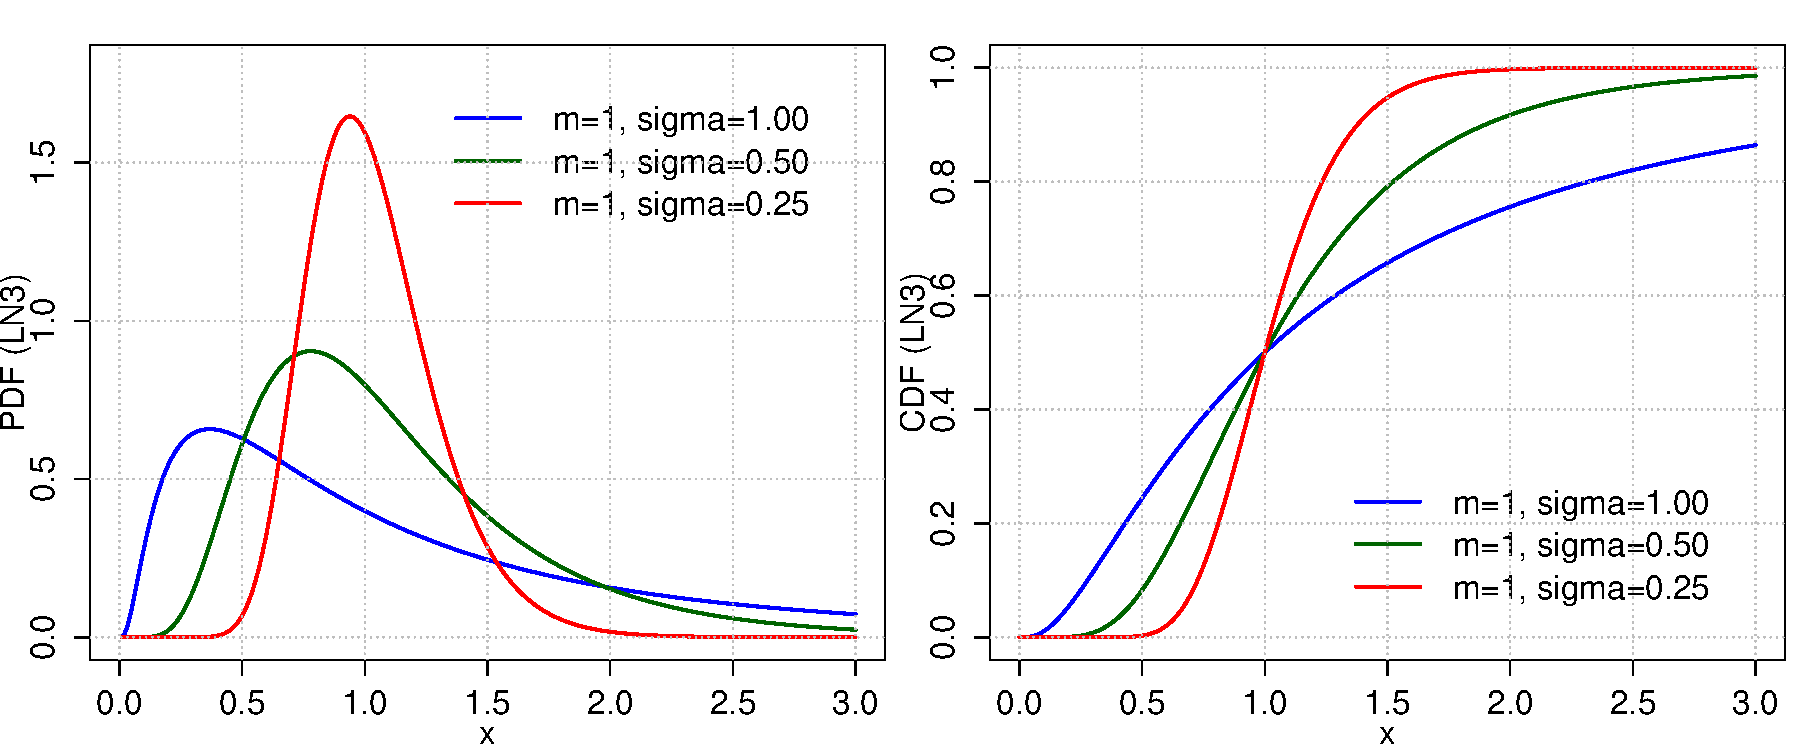
\includegraphics[width=140mm]{pics/LogNormal3_pdf_cdf}
 \caption{PDF and CDF of the Log-Normal distribution, LN3,
 plotted using the provided R-code.}
 \label{fig:LN3pdfcdf}
\end{figure}

\subsubsection*{Parameter: median}

\noindent\begin{tabular}{p{2cm}cl}
\textbf{name} & & median / geometric mean \\
\textbf{type} & & scalar \\
\textbf{symbol} & & $m$  \\
\textbf{definition} & & $m>0$
\end{tabular}
\subsubsection*{Parameter: stdevLog}

\noindent\begin{tabular}{p{2cm}cl}
\textbf{name} & & shape \\
\textbf{type} & & scalar \\
\textbf{symbol} & & $\sigma$  \\
\textbf{definition} & & $\sigma > 0$
\end{tabular}
\subsubsection*{Functions}

\smallskip \noindent \hspace{.2cm} \textbf{PDF} 
\begin{equation*}\frac{1}{x\sigma\sqrt{2\pi}}\ e^{-\frac{\left[\ln (x/m)\right]^2}{2\sigma^2}}\end{equation*}
\smallskip \noindent \hspace{.2cm} \textbf{PDF in R}  
\begin{verbatim}1/(x*sigma*sqrt(2*pi)) * exp(-(log(x/m))^2 / (2*sigma^2))\end{verbatim}
\smallskip \noindent \hspace{.2cm} \textbf{CDF} 
\begin{equation*}\frac12 + \frac12\,\text{erf}\Big[\frac{\ln x-\ln m}{\sqrt{2}\sigma}\Big]\end{equation*}
\smallskip \noindent \hspace{.2cm} \textbf{CDF in R} 
\begin{verbatim}1/2 + 1/2 * erf( (log(x)-log(m)) / (sqrt(2)*sigma) )\end{verbatim}
\smallskip\section*{LogNormal4} 

  \bigskip 

\begin{tabular}{p{2cm}cl}
\textbf{name} & & Log-Normal 4 (ID: 0000304)\\ 
 
\textbf{type} & & continuous \\ 

\textbf{variate} & & $x$, scalar \\ 

\textbf{support} & & $x \in (0,+\infty)$
\end{tabular}
\subsubsection*{Parameter: median}

\noindent\begin{tabular}{p{2cm}cl}
\textbf{name} & & median / geometric mean \\
\textbf{type} & & scalar \\
\textbf{symbol} & & $m$  \\
\textbf{definition} & & $m>0$
\end{tabular}
\subsubsection*{Parameter: coefVar}

\noindent\begin{tabular}{p{2cm}cl}
\textbf{name} & & coefficient of variation \\
\textbf{type} & & scalar \\
\textbf{symbol} & & $cv$  \\
\textbf{definition} & & $cv>0$
\end{tabular}

\begin{figure}[htb!]
\centering
  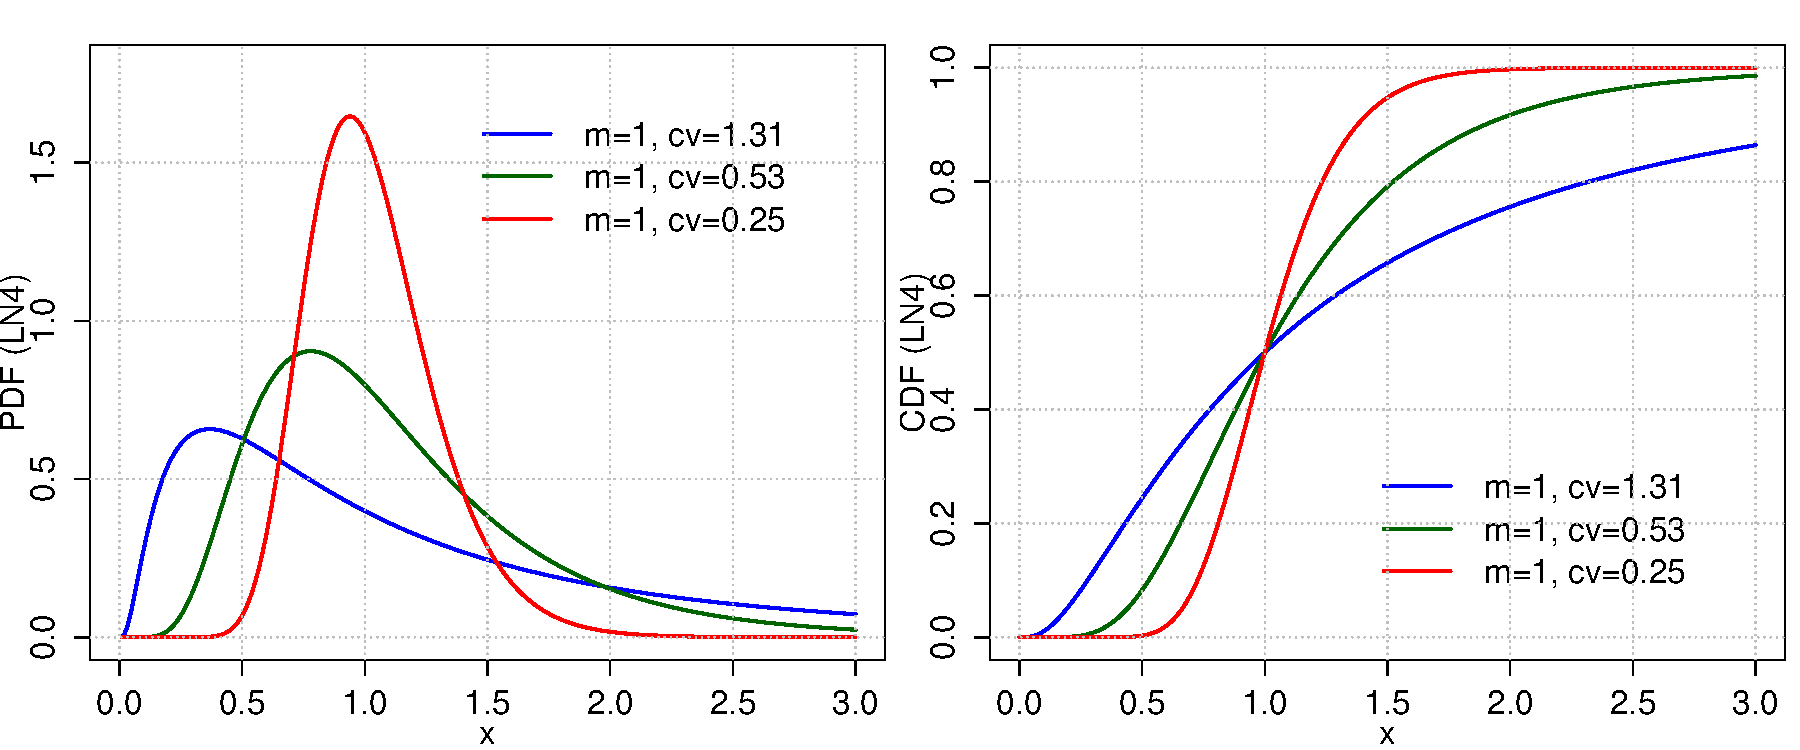
\includegraphics[width=140mm]{pics/LogNormal4_pdf_cdf.pdf}
 \caption{PDF and CDF of the Log-Normal distribution, LN4,
 plotted using the provided R-code.}
 \label{fig:LN4pdfcdf}
\end{figure}

\subsubsection*{Functions}

\smallskip \noindent \hspace{.2cm} \textbf{PDF} 
\begin{equation*}\frac{1}{x\sqrt{\ln(cv^2+1)}\sqrt{2\pi}}\ e^{-\frac{\left[\ln (x/m)\right]^2}{2\ln(cv^2+1)}}\end{equation*}
\smallskip \noindent \hspace{.2cm} \textbf{PDF in R}  
\begin{verbatim}1/(x*sqrt(log(cv^2+1))*sqrt(2*pi)) * exp( -(log(x/m))^2 / (2*log(cv^2+1)) )\end{verbatim}
\smallskip \noindent \hspace{.2cm} \textbf{CDF} 
\begin{equation*}\frac12 + \frac12\,\text{erf}\Big[\frac{\ln x-\ln m}{\sqrt{2}\sqrt{\log(cv^2+1)}}\Big]\end{equation*}
\smallskip \noindent \hspace{.2cm} \textbf{CDF in R} 
\begin{verbatim}1/2 + 1/2 * erf( (log(x)-log(m)) / (sqrt(2*log(cv^2+1))) )\end{verbatim}
\smallskip\section*{LogNormal5} 

  \bigskip 

\begin{tabular}{p{2cm}cl}
\textbf{name} & & Log-Normal 5 (ID: 0000314)\\ 
 
\textbf{type} & & continuous \\ 

\textbf{variate} & & $x$, scalar \\ 

\textbf{support} & & $x \in (0,+\infty)$
\end{tabular}
\subsubsection*{Parameter: meanLog}

\noindent\begin{tabular}{p{2cm}cl}
\textbf{name} & & mean of log(x) \\
\textbf{type} & & scalar \\
\textbf{symbol} & & $\mu$  \\
\textbf{definition} & & $\mu \in R$
\end{tabular}
\subsubsection*{Parameter: precision}

\noindent\begin{tabular}{p{2cm}cl}
\textbf{name} & & precision \\
\textbf{type} & & scalar \\
\textbf{symbol} & & $\tau$  \\
\textbf{definition} & & $\tau > 0$
\end{tabular}

\begin{figure}[htb!]
\centering
  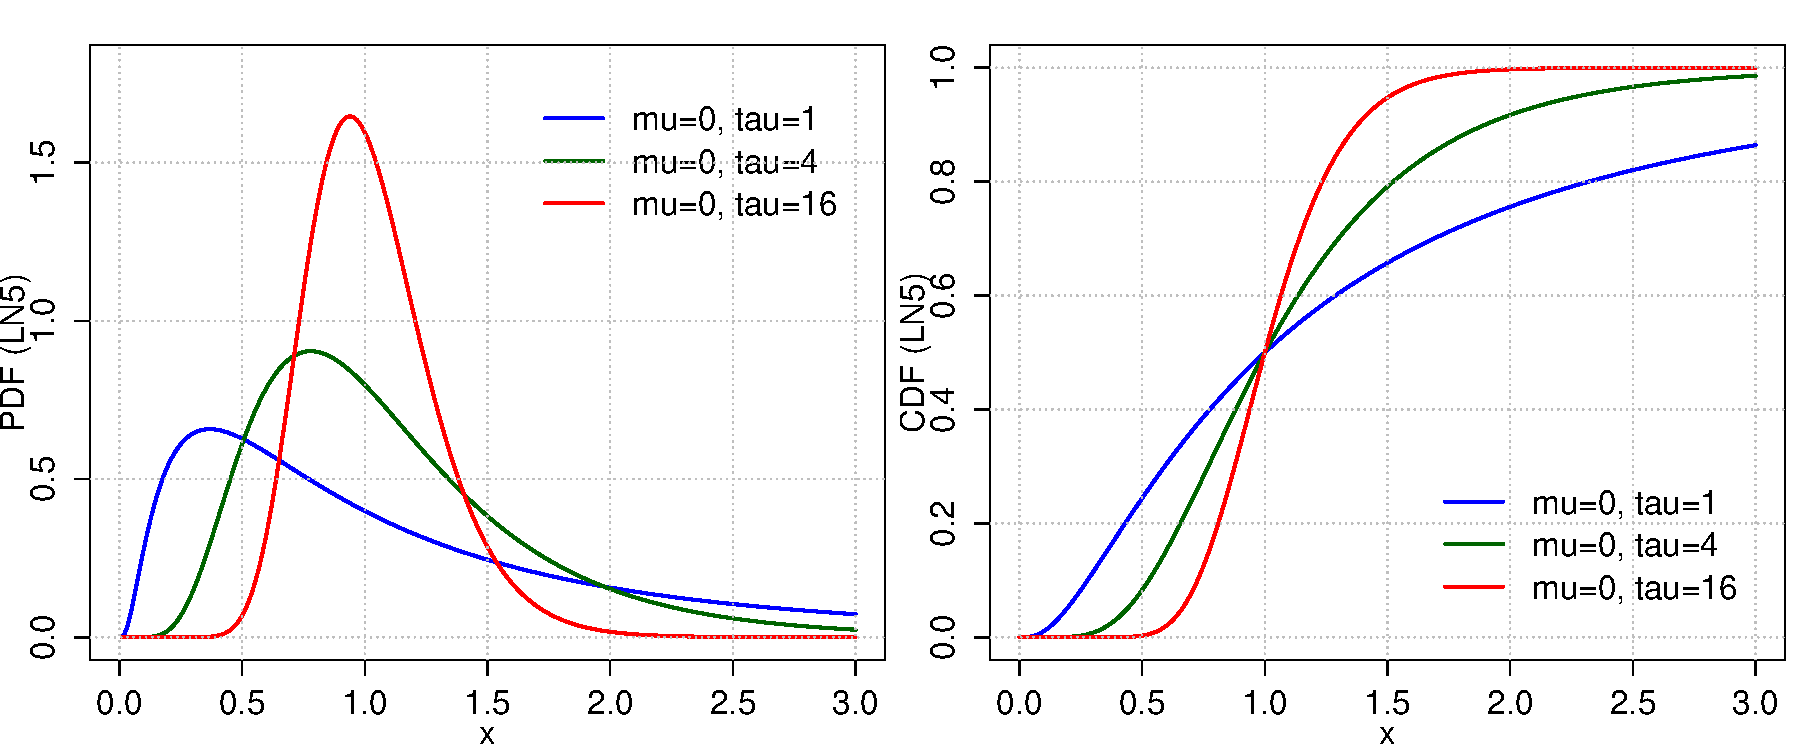
\includegraphics[width=140mm]{pics/LogNormal5_pdf_cdf.pdf}
 \caption{PDF and CDF of the Log-Normal distribution, LN5,
 plotted using the provided R-code.}
 \label{fig:LN5pdfcdf}
\end{figure}

\subsubsection*{Functions}

\smallskip \noindent \hspace{.2cm} \textbf{PDF} 
\begin{equation*}\sqrt{\frac{\tau}{2 \pi}} \frac{1}{x}e^{-\frac{\tau}{2}(\log x-\mu)^2}\end{equation*}
\smallskip \noindent \hspace{.2cm} \textbf{PDF in R}  
\begin{verbatim}sqrt(tau / (2*pi)) * (1/x) * exp(- (tau/2)*(log(x)-mu)^2 )\end{verbatim}
\smallskip \noindent \hspace{.2cm} \textbf{CDF} 
\begin{equation*}\frac12 + \frac12\,\text{erf}\Big[\frac{\ln x-\mu}{\sqrt{2/\tau}}\Big]\end{equation*}
\smallskip \noindent \hspace{.2cm} \textbf{CDF in R} 
\begin{verbatim}1/2 + 1/2 * erf( (log(x)-mu) / sqrt(2/tau) )\end{verbatim}
\smallskip\section*{LogNormal6} 

  \bigskip 

\begin{tabular}{p{2cm}cl}
\textbf{name} & & Log-Normal 6 (ID: 0000004)\\ 
 
\textbf{type} & &  \\ 

\textbf{variate} & & $$,  \\ 

\textbf{support} & & $$
\end{tabular}
\subsubsection*{Functions}

\smallskip \noindent \hspace{.2cm} \textbf{} 
\begin{equation*}\end{equation*}
\smallskip \noindent \hspace{.2cm} \textbf{CDF} 
\begin{equation*}\end{equation*}
\smallskip\section*{LogNormal7} 

  \bigskip 

\begin{tabular}{p{2cm}cl}
\textbf{name} & & Log-Normal 7 (ID: 0000017)\\ 
 
\textbf{type} & &  \\ 

\textbf{variate} & & $$,  \\ 

\textbf{support} & & $$
\end{tabular}
\subsubsection*{Functions}

\smallskip \noindent \hspace{.2cm} \textbf{} 
\begin{equation*}\end{equation*}
\smallskip \noindent \hspace{.2cm} \textbf{CDF} 
\begin{equation*}\end{equation*}
\smallskip\section*{LogUniform} 

  \bigskip 

\begin{tabular}{p{2cm}cl}
\textbf{name} & & Log-Uniform (ID: 0000029)\\ 
 
\textbf{type} & & continuous \\ 

\textbf{variate} & & $x$, scalar \\ 

\textbf{support} & & $x \in (min,max)$
\end{tabular}

\begin{figure}[htb!]
\centering
  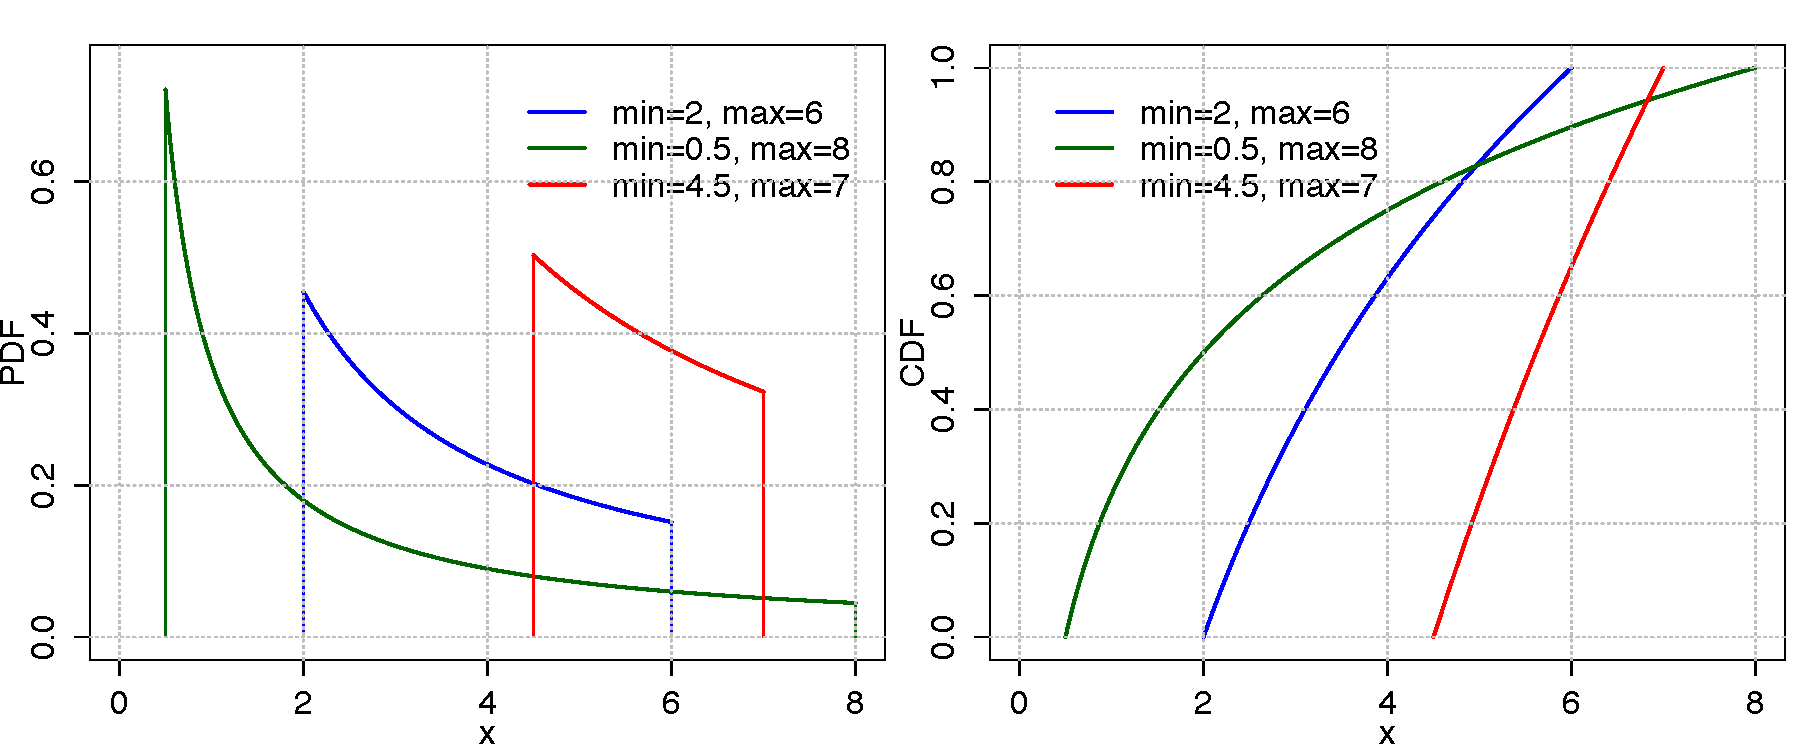
\includegraphics[width=140mm]{pics/LogUniform_pdf_cdf.pdf}
 \caption{PDF and CDF of the Log-uniform distribution plotted using the provided R-code.}
 \label{fig:LogUniform_pdf_cdf}
\end{figure}

\subsubsection*{Parameter: minimum}

\noindent\begin{tabular}{p{2cm}cl}
\textbf{name} & & minimum \\
\textbf{type} & & scalar \\
\textbf{symbol} & & $min$  \\
\textbf{definition} & & $m>0$
\end{tabular}
\subsubsection*{Parameter: maximum}

\noindent\begin{tabular}{p{2cm}cl}
\textbf{name} & & maximum \\
\textbf{type} & & scalar \\
\textbf{symbol} & & $max$  \\
\textbf{definition} & & $max \geq min$
\end{tabular}
\subsubsection*{Functions}

\smallskip \noindent \hspace{.2cm} \textbf{PDF} 
\begin{equation*}\frac{1}{x(\log(max) - \log(min))}\end{equation*}
\smallskip \noindent \hspace{.2cm} \textbf{PDF in R}  
\begin{verbatim}1/(x*(log(max) - log(min)))\end{verbatim}
\smallskip \noindent \hspace{.2cm} \textbf{CDF} 
\begin{equation*}\frac{\log(x) - \log(min)}{\log(max) - \log(min)}\end{equation*}
\smallskip \noindent \hspace{.2cm} \textbf{CDF in R} 
\begin{verbatim}(log(x) - log(min)) / (log(max) - log(min))\end{verbatim}
\smallskip\section*{Logistic} 

  \bigskip 

\begin{tabular}{p{2cm}cl}
\textbf{name} & & Logistic (ID: 0000253)\\ 
 
\textbf{type} & & continuous \\ 

\textbf{variate} & & $x$, scalar \\ 

\textbf{support} & & $x \in (-\infty,+\infty)$
\end{tabular}

\begin{figure}[htb!]
\centering
  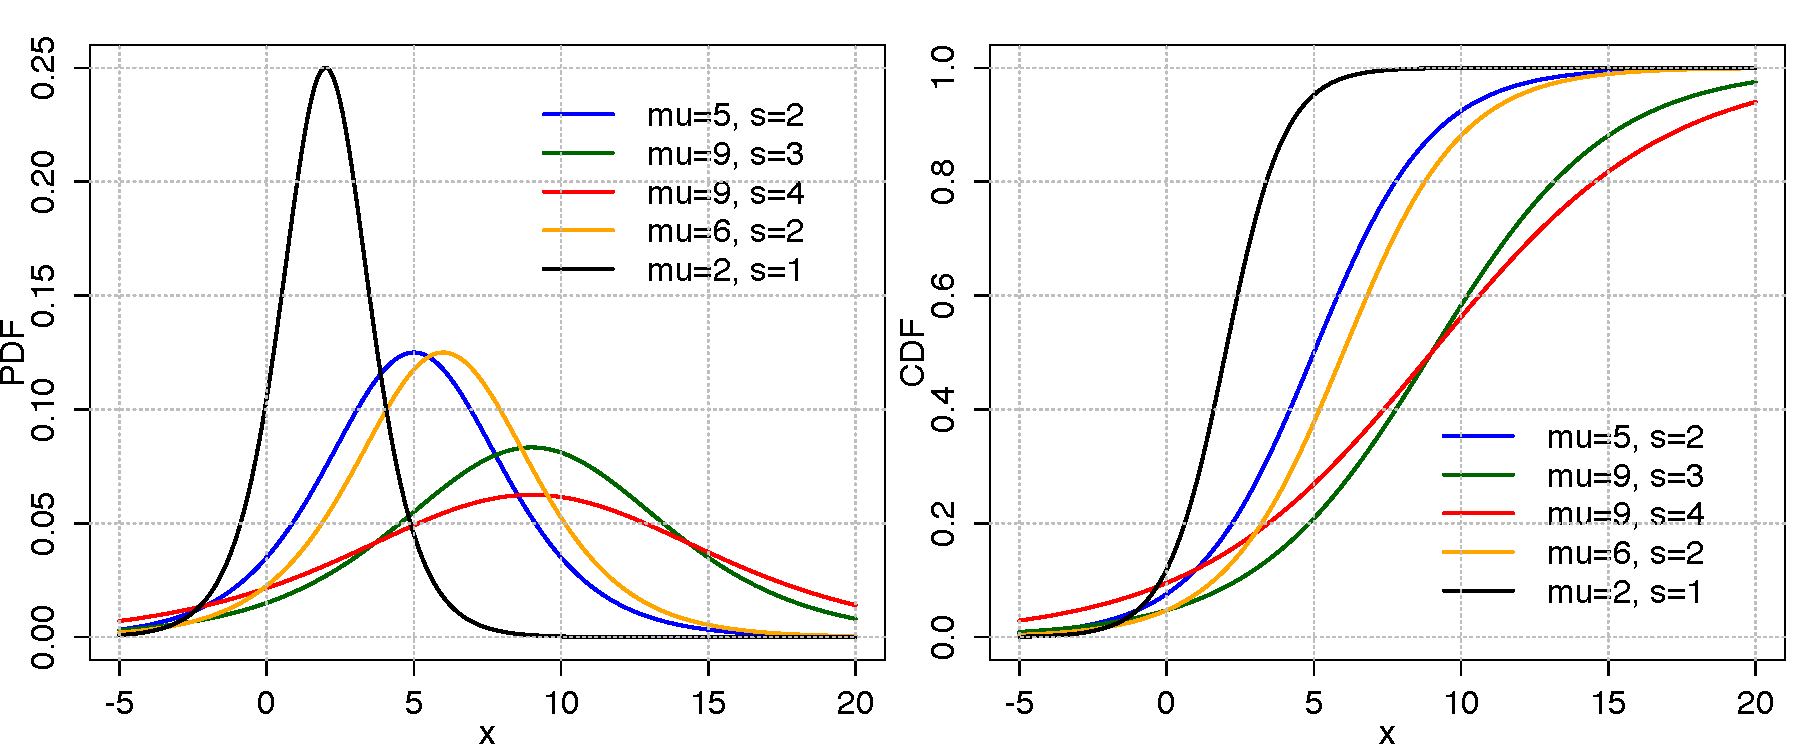
\includegraphics[width=140mm]{pics/Logistic_pdf_cdf.pdf}
 \caption{PDF and CDF of the Logistic distribution plotted using the provided R-code.}
 \label{fig:Logistic_pdf_cdf}
\end{figure}

\subsubsection*{Parameter: location}

\noindent\begin{tabular}{p{2cm}cl}
\textbf{name} & & location \\
\textbf{type} & & scalar \\
\textbf{symbol} & & $\mu$  \\
\textbf{definition} & & $\mu \in R$
\end{tabular}
\subsubsection*{Parameter: scale}

\noindent\begin{tabular}{p{2cm}cl}
\textbf{name} & & scale \\
\textbf{type} & & scalar \\
\textbf{symbol} & & $s$  \\
\textbf{definition} & & $s > 0, s \in R$
\end{tabular}
\subsubsection*{Functions}

\smallskip \noindent \hspace{.2cm} \textbf{PDF} 
\begin{equation*}\frac{e^{-\frac{x-\mu}{s}}} {s\left(1+e^{-\frac{x-\mu}{s}}\right)^2}\end{equation*}
\smallskip \noindent \hspace{.2cm} \textbf{PDF in R}  
\begin{verbatim}exp(-(x-mu)/s) / (s*(1+exp(-(x-mu)/s))^2)\end{verbatim}
\smallskip \noindent \hspace{.2cm} \textbf{CDF} 
\begin{equation*}\frac{1}{1+e^{-\frac{x-\mu}{s}}}\end{equation*}
\smallskip \noindent \hspace{.2cm} \textbf{CDF in R} 
\begin{verbatim}1/(1+exp(-(x-mu)/s))\end{verbatim}
\smallskip\section*{MixtureDistribution} 

  \bigskip 

\begin{tabular}{p{2cm}cl}
\textbf{name} & & Mixture Distribution (ID: 0000039)\\ 
 
\textbf{type} & & continuous \\ 

\textbf{variate} & & $-$, - \\ 

\textbf{support} & & $-$
\end{tabular}
\subsubsection*{Parameter: weight}

\noindent\begin{tabular}{p{2cm}cl}
\textbf{name} & & mixing coefficients \\
\textbf{type} & & vector \\
\textbf{symbol} & & $\pi_1, \ldots, \pi_k$  \\
\textbf{definition} & & $\Sigma_{i=1}^K \pi_i=1; 0\le \pi_i \le 1$
\end{tabular}
\subsubsection*{Functions}

\smallskip \noindent \hspace{.2cm} \textbf{PDF} 
\begin{equation*}f(x; \pi, \theta) = \sum_{i=1}^{K} \pi_{i}\; p_i(x; \theta_i) \text{ where } p_i(x; \theta_i) \text{the PDF of the } i^{th} \text{ component with parameters } \theta_i\end{equation*}
\smallskip \noindent \hspace{.2cm} \textbf{CDF} 
\begin{equation*}-\end{equation*}
\smallskip\section*{Multinomial} 

  \bigskip 

\begin{tabular}{p{2cm}cl}
\textbf{name} & & Multinomial (ID: 0000048)\\ 
 
\textbf{type} & & discrete \\ 

\textbf{variate} & & $X$, vector \\ 

\textbf{support} & & $X_i \in \{0,\dots,n\}, \Sigma X_i = n$
\end{tabular}
\subsubsection*{Parameter: numberOfTrials}

\noindent\begin{tabular}{p{2cm}cl}
\textbf{name} & & number of trials \\
\textbf{type} & & scalar \\
\textbf{symbol} & & $n$  \\
\textbf{definition} & & $n > 0, n \in N$
\end{tabular}
\subsubsection*{Parameter: probabilityOfSuccess}

\noindent\begin{tabular}{p{2cm}cl}
\textbf{name} & & event probabilities \\
\textbf{type} & & vector \\
\textbf{symbol} & & $p_1, \ldots, p_k$  \\
\textbf{definition} & & $p_1, \ldots, p_k, \Sigma p_i = 1$
\end{tabular}
\subsubsection*{Functions}

\smallskip \noindent \hspace{.2cm} \textbf{PMF} 
\begin{equation*}\frac{n!}{x_1!\cdots x_k!} p_1^{x_1} \cdots p_k^{x_k}\end{equation*}
\smallskip \noindent \hspace{.2cm} \textbf{CDF} 
\begin{equation*}-\end{equation*}
\smallskip\section*{MultivariateNormal1} 

  \bigskip 

\begin{tabular}{p{2cm}cl}
\textbf{name} & & Multivariate Normal 1 (ID: 0000057)\\ 
 
\textbf{type} & & continuous \\ 

\textbf{variate} & & $x$, vector \\ 

\textbf{support} & & $x \in \mu + \text{span}(\Sigma) \subseteq  R^k$
\end{tabular}
\subsubsection*{Parameter: mean}

\noindent\begin{tabular}{p{2cm}cl}
\textbf{name} & & location \\
\textbf{type} & & vector \\
\textbf{symbol} & & $\mu$  \\
\textbf{definition} & & $\mu \in R^k$
\end{tabular}
\subsubsection*{Parameter: covarianceMatrix}

\noindent\begin{tabular}{p{2cm}cl}
\textbf{name} & & covariance matrix \\
\textbf{type} & & matrix \\
\textbf{symbol} & & $\Sigma$  \\
\textbf{definition} & & $\Sigma \in R^{k\times k}$
\end{tabular}
\subsubsection*{Functions}

\smallskip \noindent \hspace{.2cm} \textbf{PDF} 
\begin{equation*}(2\pi)^{-\frac{k}{2}}|\Sigma|^{-\frac{1}{2}}\, e^{ -\frac{1}{2}(x-\mu)'\Sigma^{-1}(x-\mu) }\end{equation*}
\smallskip \noindent \hspace{.2cm} \textbf{CDF} 
\begin{equation*}\text{no analytic expression}\end{equation*}
\smallskip\section*{MultivariateNormal2} 

  \bigskip 

\begin{tabular}{p{2cm}cl}
\textbf{name} & & Multivariate Normal 2 (ID: 0000067)\\ 
 
\textbf{type} & & continuous \\ 

\textbf{variate} & & $x$, vector \\ 

\textbf{support} & & $x \in \mu + \text{span}(\Sigma) \subseteq  R^k$
\end{tabular}
\subsubsection*{Parameter: mean}

\noindent\begin{tabular}{p{2cm}cl}
\textbf{name} & & location \\
\textbf{type} & & vector \\
\textbf{symbol} & & $\mu$  \\
\textbf{definition} & & $\mu \in R^k$
\end{tabular}
\subsubsection*{Parameter: precisionMatrix}

\noindent\begin{tabular}{p{2cm}cl}
\textbf{name} & & precision matrix \\
\textbf{type} & & matrix \\
\textbf{symbol} & & $T$  \\
\textbf{definition} & & $-$
\end{tabular}
\subsubsection*{Functions}

\smallskip \noindent \hspace{.2cm} \textbf{PDF} 
\begin{equation*}(2\pi)^{-d/2}|T|^{\frac{1}{2}}\, \exp\big( -\frac{1}{2}(x-\mu)' T (x-\mu) \big)\end{equation*}
\smallskip \noindent \hspace{.2cm} \textbf{CDF} 
\begin{equation*}\text{no analytic expression}\end{equation*}
\smallskip\section*{MultivariateStudentT1} 

  \bigskip 

\begin{tabular}{p{2cm}cl}
\textbf{name} & & Multivariate (Student) T 1 (ID: 0000076)\\ 
 
\textbf{type} & & continuous \\ 

\textbf{variate} & & $x$, vector \\ 

\textbf{support} & & $x \in R^p$
\end{tabular}
\subsubsection*{Parameter: mean}

\noindent\begin{tabular}{p{2cm}cl}
\textbf{name} & & location \\
\textbf{type} & & vector \\
\textbf{symbol} & & $\mu$  \\
\textbf{definition} & & $\mu = [\mu_1, \dots, \mu_p]^T, \mu_i \in R$
\end{tabular}
\subsubsection*{Parameter: covarianceMatrix}

\noindent\begin{tabular}{p{2cm}cl}
\textbf{name} & & covariance matrix \\
\textbf{type} & & matrix \\
\textbf{symbol} & & $\Sigma$  \\
\textbf{definition} & & $\Sigma, \text{ positive-definite real } p\times p \text{ matrix}$
\end{tabular}
\subsubsection*{Parameter: degreesOfFreedom}

\noindent\begin{tabular}{p{2cm}cl}
\textbf{name} & & degrees of freedom \\
\textbf{type} & & scalar \\
\textbf{symbol} & & $\nu$  \\
\textbf{definition} & & $\nu$
\end{tabular}
\subsubsection*{Functions}

\smallskip \noindent \hspace{.2cm} \textbf{PDF} 
\begin{equation*}\frac{\Gamma\left[(\nu+p)/2\right]}{\Gamma(\nu/2)\nu^{p/2}\pi^{p/2}\left|\Sigma\right|^{1/2}\left[1+\frac{1}{\nu}(x-\mu)^{\rm T}\Sigma^{-1}(x-\mu)\right]^{(\nu+p)/2}}\end{equation*}
\smallskip \noindent \hspace{.2cm} \textbf{CDF} 
\begin{equation*}\text{no analytic expression}\end{equation*}
\smallskip\section*{MultivariateStudentT2} 

  \bigskip 

\begin{tabular}{p{2cm}cl}
\textbf{name} & & Multivariate (Student) T 2 (ID: 0000084)\\ 
 
\textbf{type} & & continuous \\ 

\textbf{variate} & & $x$, vector \\ 

\textbf{support} & & $x \in R^p, k\geq 2$
\end{tabular}
\subsubsection*{Parameter: mean}

\noindent\begin{tabular}{p{2cm}cl}
\textbf{name} & & location \\
\textbf{type} & & vector \\
\textbf{symbol} & & $\mu$  \\
\textbf{definition} & & $\mu = [\mu_1, \dots, \mu_p]^T, \mu_i \in R$
\end{tabular}
\subsubsection*{Parameter: precisionMatrix}

\noindent\begin{tabular}{p{2cm}cl}
\textbf{name} & & precision matrix \\
\textbf{type} & & matrix \\
\textbf{symbol} & & $T$  \\
\textbf{definition} & & $-$
\end{tabular}
\subsubsection*{Parameter: degreesOfFreedom}

\noindent\begin{tabular}{p{2cm}cl}
\textbf{name} & & degrees of freedom \\
\textbf{type} & & scalar \\
\textbf{symbol} & & $k$  \\
\textbf{definition} & & $-$
\end{tabular}
\subsubsection*{Functions}

\smallskip \noindent \hspace{.2cm} \textbf{PDF} 
\begin{equation*}\frac{\Gamma((k+d)/2)}{\Gamma(k/2) k^{d/2} \pi^{d/2}}|T|^{1/2} \Big[ 1 + \frac{1}{k}(x-\mu)' T (x-\mu) \Big]^{-(k+d)/2}\end{equation*}
\smallskip \noindent \hspace{.2cm} \textbf{CDF} 
\begin{equation*}-\end{equation*}
\smallskip\section*{Nakagami} 

  \bigskip 

\begin{tabular}{p{2cm}cl}
\textbf{name} & & Nakagami (ID: 0000094)\\ 
 
\textbf{type} & & continuous \\ 

\textbf{variate} & & $x$, scalar \\ 

\textbf{support} & & $x \in (0,+\infty)$
\end{tabular}

\begin{figure}[htb!]
\centering
  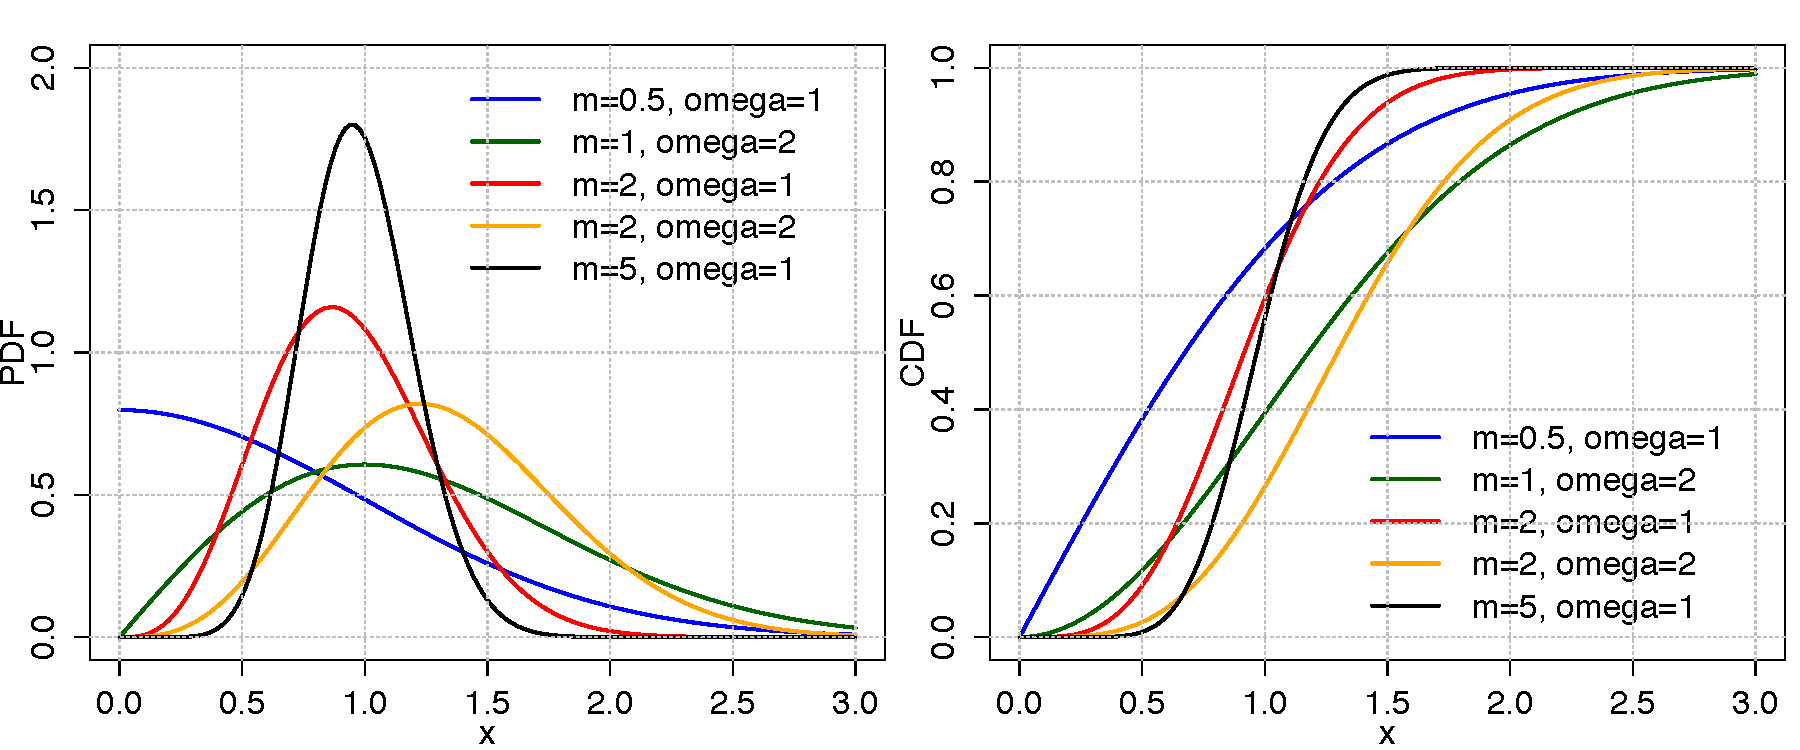
\includegraphics[width=140mm]{pics/Nakagami_pdf_cdf.pdf}
 \caption{PDF and CDF of the Nakagami distribution plotted using the provided R-code.}
 \label{fig:Nakagami_pdf_cdf}
\end{figure}

\subsubsection*{Parameter: shape}

\noindent\begin{tabular}{p{2cm}cl}
\textbf{name} & & shape \\
\textbf{type} & & scalar \\
\textbf{symbol} & & $m$  \\
\textbf{definition} & & $m > 0$
\end{tabular}
\subsubsection*{Parameter: spread}

\noindent\begin{tabular}{p{2cm}cl}
\textbf{name} & & spread \\
\textbf{type} & & scalar \\
\textbf{symbol} & & $\Omega$  \\
\textbf{definition} & & $ \Omega > 0$
\end{tabular}
\subsubsection*{Functions}

\smallskip \noindent \hspace{.2cm} \textbf{PDF} 
\begin{equation*}\frac{2m^m}{\Gamma(m)\Omega^m}x^{2m-1} \exp(-\frac{m}{\omega}x^2)\end{equation*}
\smallskip \noindent \hspace{.2cm} \textbf{PDF in R}  
\begin{verbatim}2*m^m / (gamma(m)*Omega^m)*x^(2*m-1)*exp(-m/Omega*x^2)\end{verbatim}
\smallskip \noindent \hspace{.2cm} \textbf{CDF} 
\begin{equation*}\frac{\gamma(m,\frac{m}{\Omega}x^2)}{\Gamma(m)}\end{equation*}
\smallskip \noindent \hspace{.2cm} \textbf{CDF in R} 
\begin{verbatim}Igamma(m,m/Omega*x^2,lower=T)/gamma(m)\end{verbatim}
\smallskip\section*{NegativeBinomial1} 

  \bigskip 

\begin{tabular}{p{2cm}cl}
\textbf{name} & & Negative Binomial 1 (ID: 0000103)\\ 
 
\textbf{type} & & discrete \\ 

\textbf{variate} & & $k$, scalar \\ 

\textbf{support} & & $k \in \{0,1,2,3,\dots\}$
\end{tabular}
\subsubsection*{Parameter: numberOfFailures}

\noindent\begin{tabular}{p{2cm}cl}
\textbf{name} & & number of failures \\
\textbf{type} & & scalar \\
\textbf{symbol} & & $r$  \\
\textbf{definition} & & $r > 0, r \in N$
\end{tabular}
\subsubsection*{Parameter: probability}

\noindent\begin{tabular}{p{2cm}cl}
\textbf{name} & & success probability \\
\textbf{type} & & scalar \\
\textbf{symbol} & & $p$  \\
\textbf{definition} & & $p \in [0,1]$
\end{tabular}

\begin{figure}[htb!]
\centering
  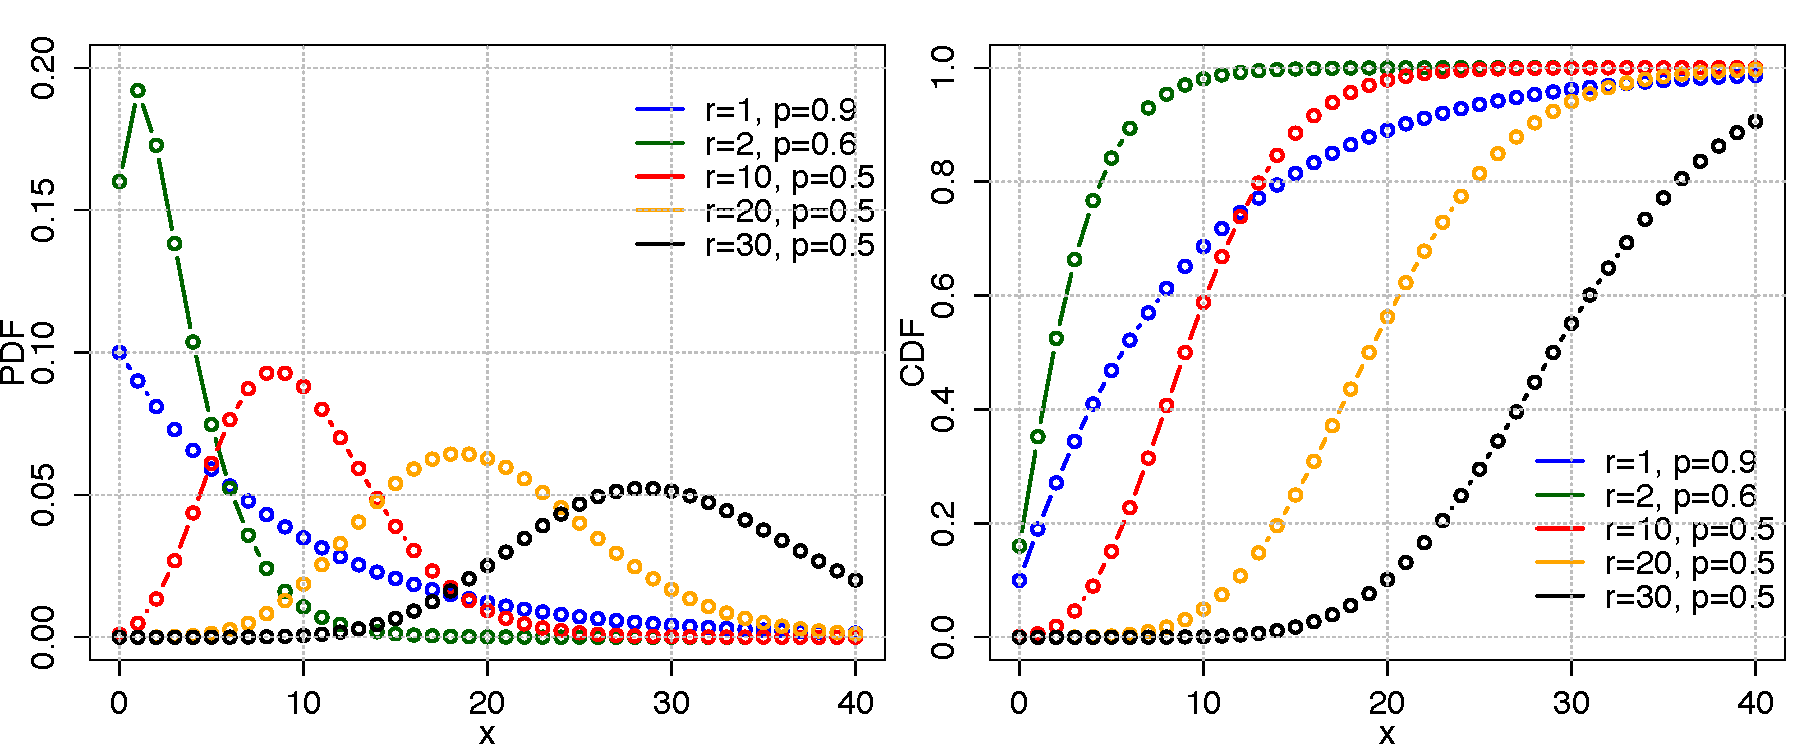
\includegraphics[width=140mm]{pics/NB1_pmf_cdf.pdf}
 \caption{PMF and CDF of the Negative Binomial distribution, NB1,
plotted using the provided R-code.}
 \label{fig:NB1pmfcdf}
\end{figure}

\subsubsection*{Functions}

\smallskip \noindent \hspace{.2cm} \textbf{PMF} 
\begin{equation*}\binom {k+r-1}k (1-p)^r p^k\end{equation*}
\smallskip \noindent \hspace{.2cm} \textbf{PMF in R}  
\begin{verbatim}choose(k+r-1,k)*(1-p)^r*p^k\end{verbatim}
\smallskip \noindent \hspace{.2cm} \textbf{CDF} 
\begin{equation*}1 - I_{p}(k+1, r)\end{equation*}
\smallskip \noindent \hspace{.2cm} \textbf{CDF in R} 
\begin{verbatim}1 - Rbeta(p, k+1, r)\end{verbatim}
\smallskip\section*{NegativeBinomial2} 

  \bigskip 

\begin{tabular}{p{2cm}cl}
\textbf{name} & & Negative Binomial 2 (ID: 0000113)\\ 
 
\textbf{type} & & discrete \\ 

\textbf{variate} & & $k$, scalar \\ 

\textbf{support} & & $k \in \{0,1,2,3,\dots\}$
\end{tabular}
\subsubsection*{Parameter: rate}

\noindent\begin{tabular}{p{2cm}cl}
\textbf{name} & & Poisson intensity \\
\textbf{type} & & scalar \\
\textbf{symbol} & & $\lambda$  \\
\textbf{definition} & & $\lambda \in R, \lambda > 0$
\end{tabular}

\begin{figure}[htb!]
\centering
  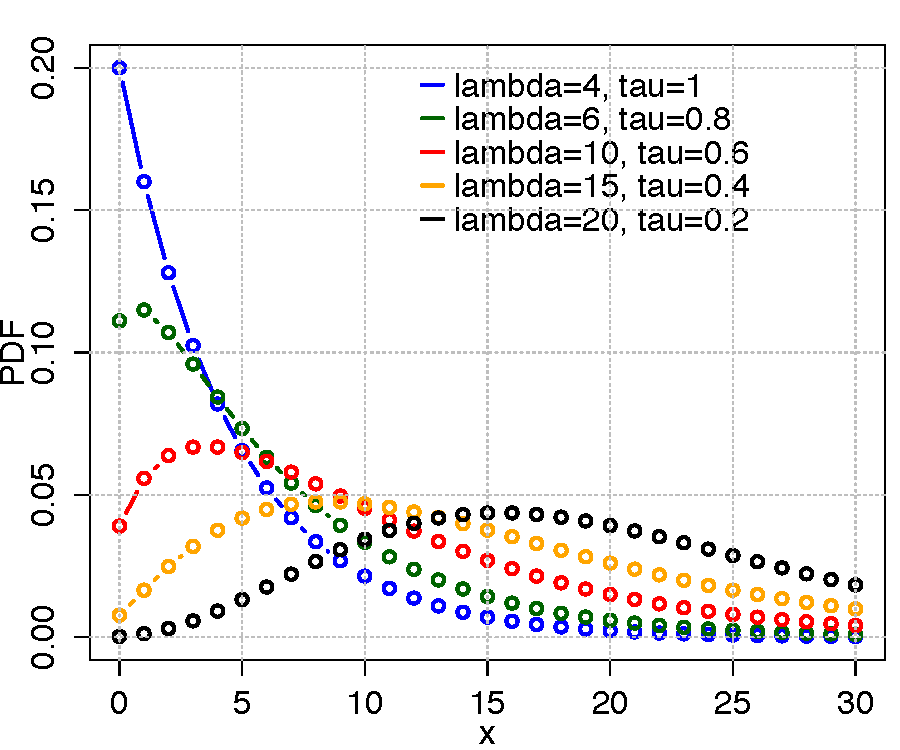
\includegraphics[width=70mm]{pics/NB2_pmf.pdf}
 \caption{PMF of the Negative Binomial distribution, NB2,
plotted using the provided R-code.}
 \label{fig:NB2pmf}
\end{figure}

\subsubsection*{Parameter: overdispersion}

\noindent\begin{tabular}{p{2cm}cl}
\textbf{name} & & overdispersion \\
\textbf{type} & & scalar \\
\textbf{symbol} & & $\tau$  \\
\textbf{definition} & & $\tau \in R$
\end{tabular}
\subsubsection*{Functions}

\smallskip \noindent \hspace{.2cm} \textbf{PMF} 
\begin{equation*}\frac{\Gamma(k + \frac{1}{\tau})}{k!\; \Gamma(\frac{1}{\tau})} \Big(\frac{1}{1+\tau \lambda} \Big)^{\frac{1}{\tau}} 
\Big(\frac{\lambda}{\frac{1}{\tau} + \lambda} \Big)^{k}\end{equation*}
\smallskip \noindent \hspace{.2cm} \textbf{PMF in R}  
\begin{verbatim}gamma(k + 1/tau)/(factorial(k) * gamma(1/tau)) * 1/(1+tau*lambda)^(1/tau) * (lambda/(1/tau + lambda))^k\end{verbatim}
\smallskip \noindent \hspace{.2cm} \textbf{CDF} 
\begin{equation*}-\end{equation*}
%\smallskip\section*{NegativeBinomial3} 
%
%  \bigskip 
%
%\begin{tabular}{p{2cm}cl}
%\textbf{name} & & Negative Binomial 3 (ID: 0000123)\\ 
% 
%\textbf{type} & & discrete \\ 
%
%\textbf{variate} & & $y$, scalar \\ 
%
%\textbf{support} & & $y \in \{0,1,2,3,\dots\}$
%\end{tabular}
%\subsubsection*{Parameter: }
%
%\noindent\begin{tabular}{p{2cm}cl}
%\textbf{name} & & mean \\
%\textbf{type} & & scalar \\
%\textbf{symbol} & & $\mu$  \\
%\textbf{definition} & & $-$
%\end{tabular}
%\subsubsection*{Parameter: -}
%
%\noindent\begin{tabular}{p{2cm}cl}
%\textbf{name} & & size parameter \\
%\textbf{type} & & scalar \\
%\textbf{symbol} & & $\theta$  \\
%\textbf{definition} & & $-$
%\end{tabular}
%\subsubsection*{Functions}
%
%\smallskip \noindent \hspace{.2cm} \textbf{PMF} 
%\begin{equation*}\frac{\Gamma(\theta + y)}{\Gamma(a)\Gamma(y+1)} \Big(\frac{\theta}{\theta + \mu} \Big)^{\theta} 
%\Big(\frac{\mu}{\theta + \mu} \Big)^{y}\end{equation*}
%\smallskip \noindent \hspace{.2cm} \textbf{CDF} 
%\begin{equation*}-\end{equation*}
\smallskip\section*{Normal1} 

  \bigskip 

\begin{tabular}{p{2cm}cl}
\textbf{name} & & Normal 1 (ID: 0000132)\\ 
 
\textbf{type} & & continuous \\ 

\textbf{variate} & & $x$, scalar \\ 

\textbf{support} & & $x \in R$
\end{tabular}
\subsubsection*{Parameter: mean}

\noindent\begin{tabular}{p{2cm}cl}
\textbf{name} & & mean \\
\textbf{type} & & scalar \\
\textbf{symbol} & & $\mu$  \\
\textbf{definition} & & $\mu \in R$
\end{tabular}

\begin{figure}[htb!]
\centering
  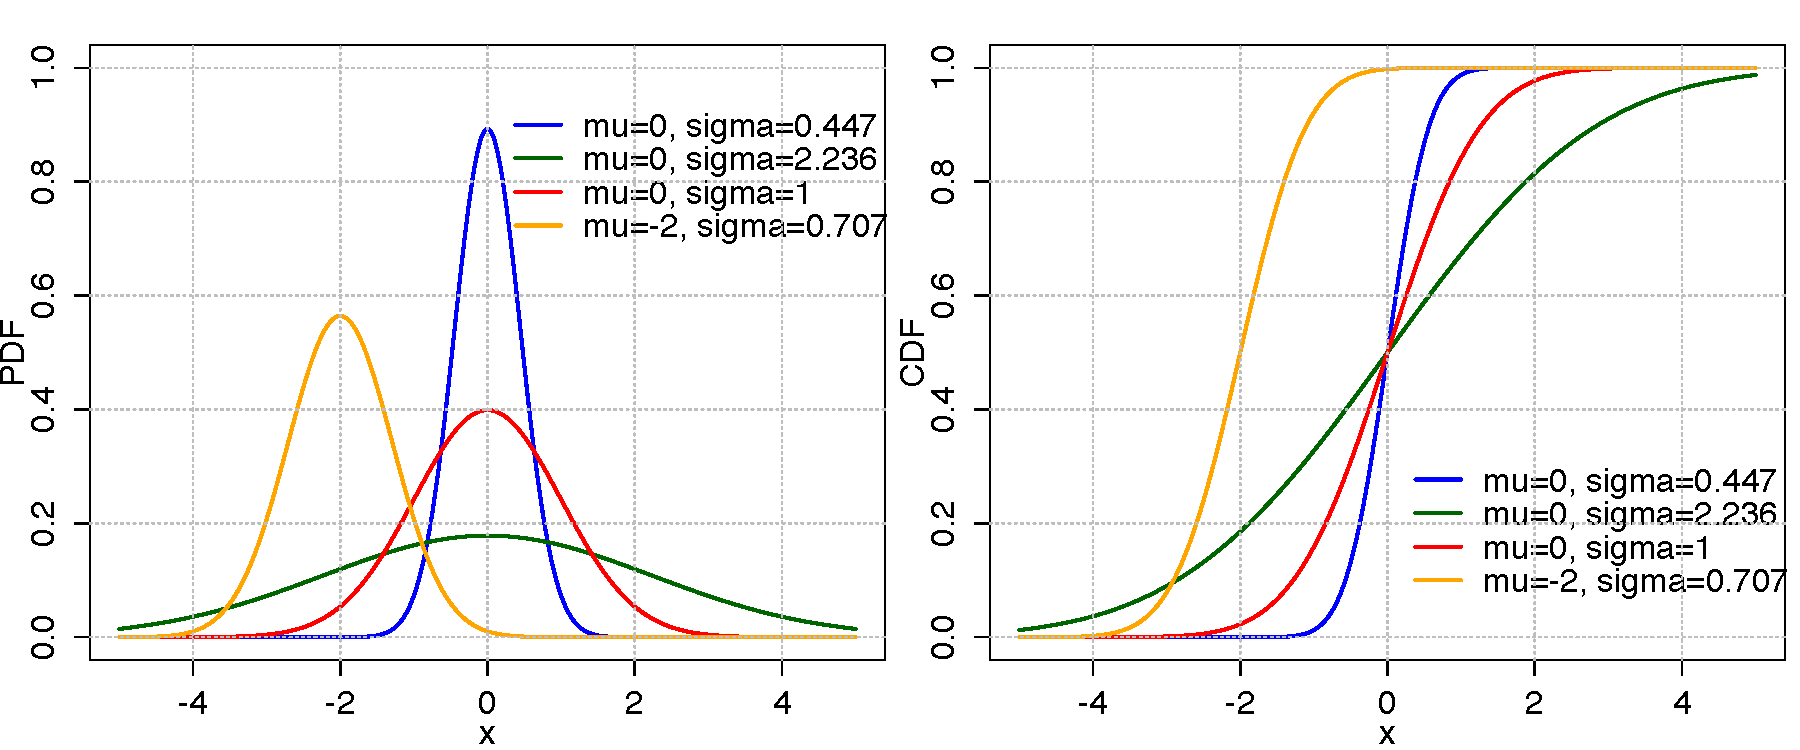
\includegraphics[width=140mm]{pics/Normal1_pdf_cdf.pdf}
 \caption{PDF and CDF of the Normal distribution, N1,
 plotted using the provided R-code.}
 \label{fig:N1pdfcdf}
\end{figure}

\subsubsection*{Parameter: stdev}

\noindent\begin{tabular}{p{2cm}cl}
\textbf{name} & & standard deviation \\
\textbf{type} & & scalar \\
\textbf{symbol} & & $\sigma$  \\
\textbf{definition} & & $\sigma> 0$
\end{tabular}
\subsubsection*{Functions}

\smallskip \noindent \hspace{.2cm} \textbf{PDF} 
\begin{equation*}\frac{1}{\sigma \sqrt{2 \pi}}e^{-\frac{(x-\mu)^2}{2\sigma^2}}\end{equation*}
\smallskip \noindent \hspace{.2cm} \textbf{PDF in R}  
\begin{verbatim}1/(sigma*sqrt(2*pi))*exp(-(x-mu)^2/(2*sigma^2))\end{verbatim}
\smallskip \noindent \hspace{.2cm} \textbf{CDF} 
\begin{equation*}\frac12\left[1 + \text{erf}\left( \frac{x-\mu}{\sigma\sqrt{2}}\right)\right]\end{equation*}
\smallskip \noindent \hspace{.2cm} \textbf{CDF in R} 
\begin{verbatim}1/2 * (1 + erf((x-mu)/(sigma*sqrt(2))))\end{verbatim}
\smallskip\section*{Normal2} 

  \bigskip 

\begin{tabular}{p{2cm}cl}
\textbf{name} & & Normal 2 (ID: 0000143)\\ 
 
\textbf{type} & & continuous \\ 

\textbf{variate} & & $x$, scalar \\ 

\textbf{support} & & $x \in R$
\end{tabular}

\begin{figure}[htb!]
\centering
  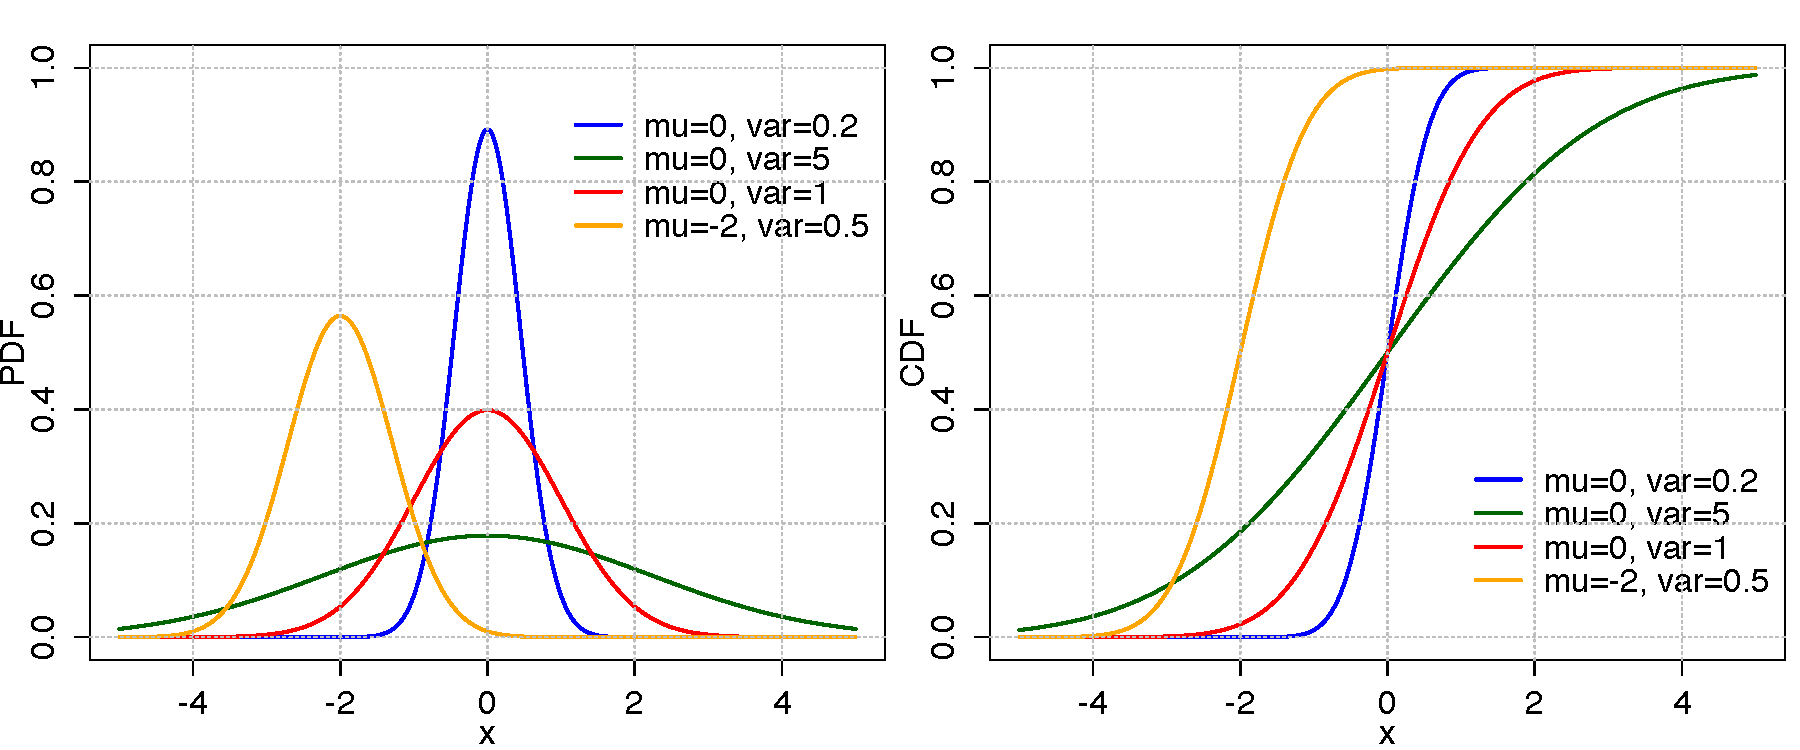
\includegraphics[width=140mm]{pics/Normal2_pdf_cdf.pdf}
 \caption{PDF and CDF of the Normal distribution, N2,
 plotted using the provided R-code.}
 \label{fig:N2pdfcdf}
\end{figure}

\subsubsection*{Parameter: mean}

\noindent\begin{tabular}{p{2cm}cl}
\textbf{name} & & mean \\
\textbf{type} & & scalar \\
\textbf{symbol} & & $\mu$  \\
\textbf{definition} & & $\mu \in R$
\end{tabular}
\subsubsection*{Parameter: var}

\noindent\begin{tabular}{p{2cm}cl}
\textbf{name} & & variance \\
\textbf{type} & & scalar \\
\textbf{symbol} & & $v$  \\
\textbf{definition} & & $v>0$
\end{tabular}
\subsubsection*{Functions}

\smallskip \noindent \hspace{.2cm} \textbf{PDF} 
\begin{equation*}\frac{1}{\sqrt{v} \sqrt{2 \pi}}e^{-\frac{(x-\mu)^2}{2*v}}\end{equation*}
\smallskip \noindent \hspace{.2cm} \textbf{PDF in R}  
\begin{verbatim}1/(sqrt(var)*sqrt(2*pi))*exp(-(x-mu)^2/(2*var))\end{verbatim}
\smallskip \noindent \hspace{.2cm} \textbf{CDF} 
\begin{equation*}\frac12\left[1 + \text{erf}\left( \frac{x-\mu}{\sqrt{v}\sqrt{2}}\right)\right]\end{equation*}
\smallskip \noindent \hspace{.2cm} \textbf{CDF in R} 
\begin{verbatim}1/2 * (1 + erf((x-mu)/(sqrt(var)*sqrt(2))))\end{verbatim}
\smallskip\section*{Normal3} 

  \bigskip 

\begin{tabular}{p{2cm}cl}
\textbf{name} & & Normal 3 (ID: 0000155)\\ 
 
\textbf{type} & & continuous \\ 

\textbf{variate} & & $x$, scalar \\ 

\textbf{support} & & $x \in R$
\end{tabular}

\begin{figure}[htb!]
\centering
  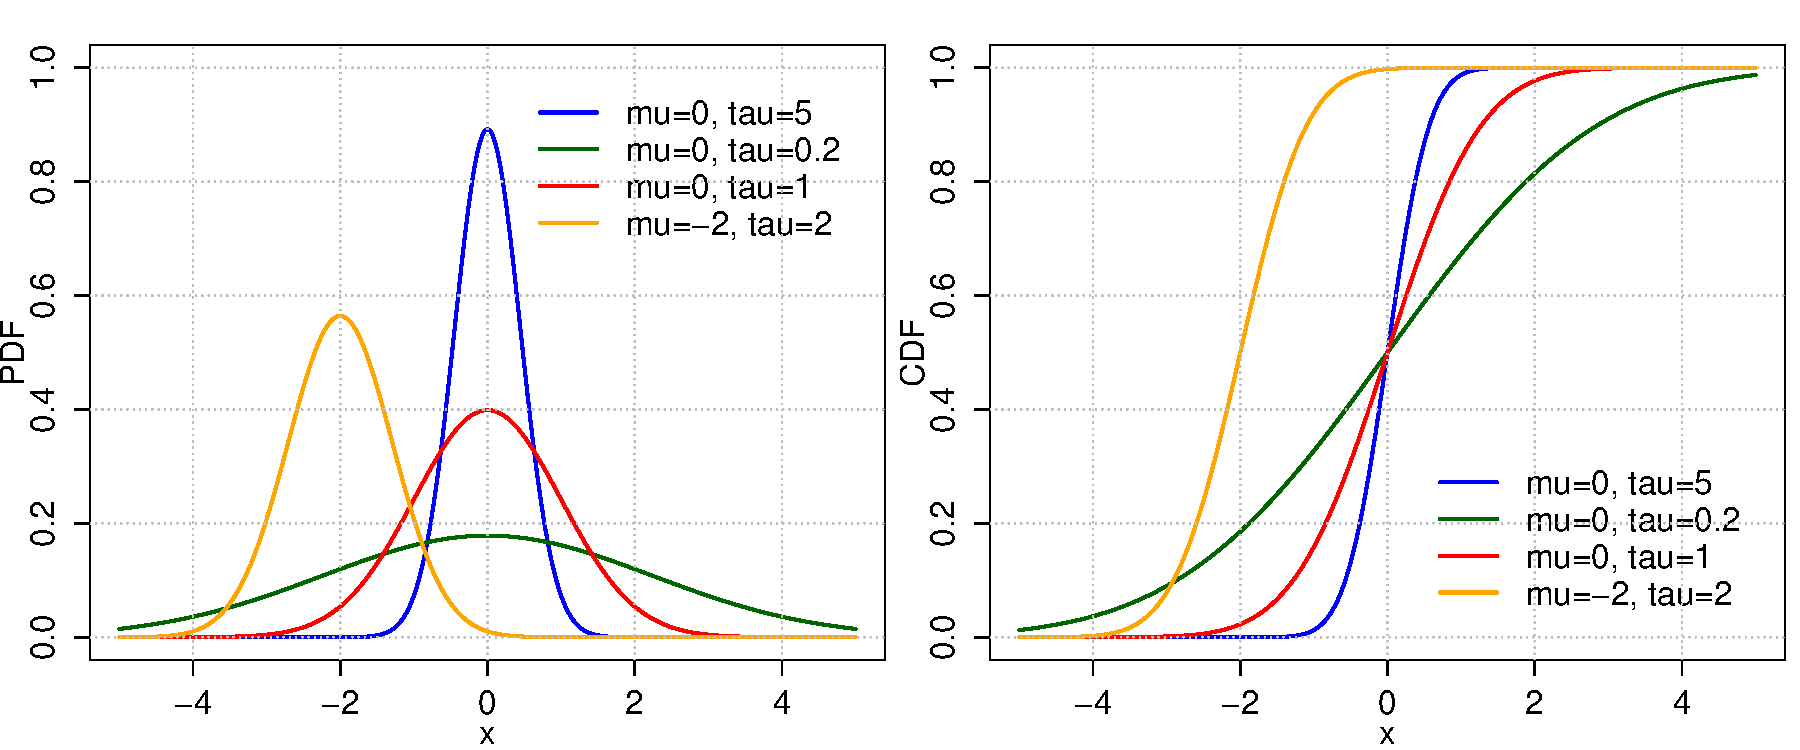
\includegraphics[width=140mm]{pics/Normal3_pdf_cdf.pdf}
 \caption{PDF and CDF of the Normal distribution, N3,
 plotted using the provided R-code.}
 \label{fig:N3pdfcdf}
\end{figure}

\subsubsection*{Parameter: mean}

\noindent\begin{tabular}{p{2cm}cl}
\textbf{name} & & mean \\
\textbf{type} & & scalar \\
\textbf{symbol} & & $\mu$  \\
\textbf{definition} & & $\mu \in R$
\end{tabular}
\subsubsection*{Parameter: precision}

\noindent\begin{tabular}{p{2cm}cl}
\textbf{name} & & precision \\
\textbf{type} & & scalar \\
\textbf{symbol} & & $\tau$  \\
\textbf{definition} & & $\tau>0$
\end{tabular}
\subsubsection*{Functions}

\smallskip \noindent \hspace{.2cm} \textbf{PDF} 
\begin{equation*}\sqrt{\frac{\tau}{2 \pi}} e^{-\frac{\tau}{2}(x-\mu)^2}\end{equation*}
\smallskip \noindent \hspace{.2cm} \textbf{PDF in R}  
\begin{verbatim}sqrt(tau/(2*pi))*exp(-tau/2*(x-mu)^2)\end{verbatim}
\smallskip \noindent \hspace{.2cm} \textbf{CDF} 
\begin{equation*}\frac12\left[1 + \text{erf}\left( \frac{x-\mu}{\sqrt{1/\tau}\sqrt{2}}\right)\right]\end{equation*}
\smallskip \noindent \hspace{.2cm} \textbf{CDF in R} 
\begin{verbatim}1/2*(1+erf((x-mu)/(sqrt(1/tau)*sqrt(2)))) \end{verbatim}
\smallskip\section*{NormalInverseGamma} 

  \bigskip 

\begin{tabular}{p{2cm}cl}
\textbf{name} & & Normal- inverse-gamma (ID: 0000165)\\ 
 
\textbf{type} & & continuous \\ 

\textbf{variate} & & $x$, scalar \\ 

\textbf{support} & & $x \in (-\infty,+\infty), \sigma^2 \in (0,+\infty)$
\end{tabular}
\subsubsection*{Parameter: mean}

\noindent\begin{tabular}{p{2cm}cl}
\textbf{name} & & location \\
\textbf{type} & & scalar \\
\textbf{symbol} & & $\mu$  \\
\textbf{definition} & & $\mu \in  R$
\end{tabular}

\begin{figure}[htb!]
\centering
  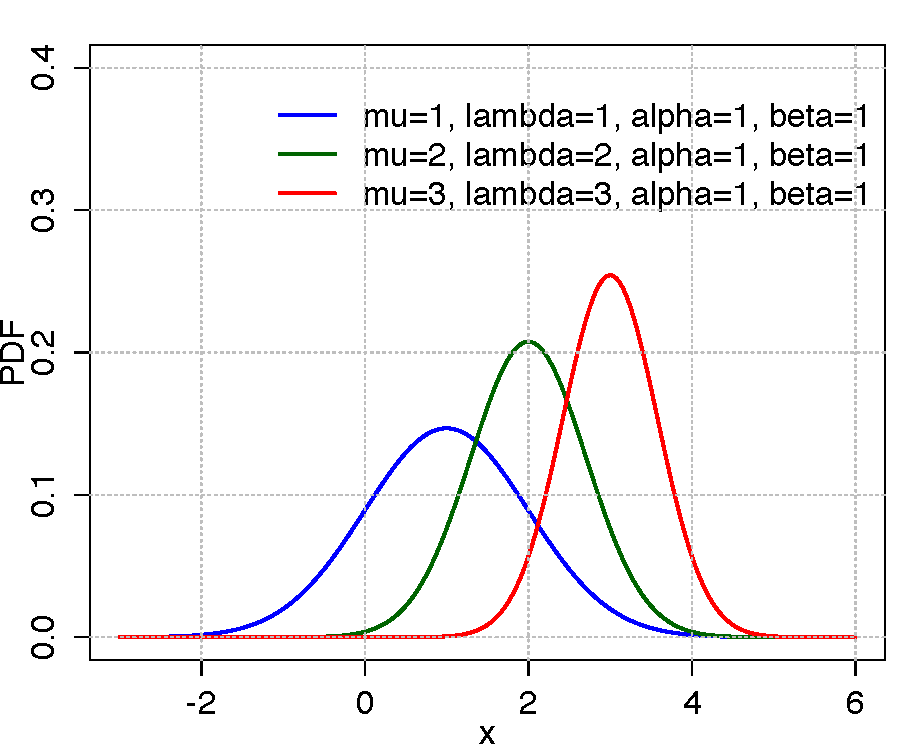
\includegraphics[width=70mm]{pics/NormalInverseGamma_pdf_cdf.pdf}
 \caption{PDF and CDF of the Normal-Inverse-Gamma distribution plotted using the provided R-code.}
 \label{fig:NormalInverseGamma_pdf_cdf}
\end{figure}

\subsubsection*{Parameter: lambda}

\noindent\begin{tabular}{p{2cm}cl}
\textbf{name} & & - \\
\textbf{type} & & scalar \\
\textbf{symbol} & & $\lambda$  \\
\textbf{definition} & & $\lambda > 0, \lambda \in  R$
\end{tabular}
\subsubsection*{Parameter: alpha}

\noindent\begin{tabular}{p{2cm}cl}
\textbf{name} & & shape \\
\textbf{type} & & scalar \\
\textbf{symbol} & & $\alpha$  \\
\textbf{definition} & & $\alpha > 0, \alpha \in  R$
\end{tabular}
\subsubsection*{Parameter: beta}

\noindent\begin{tabular}{p{2cm}cl}
\textbf{name} & & scale \\
\textbf{type} & & scalar \\
\textbf{symbol} & & $\beta$  \\
\textbf{definition} & & $\beta > 0, \beta \in  R$
\end{tabular}
\subsubsection*{Functions}

\smallskip \noindent \hspace{.2cm} \textbf{PDF} 
\begin{equation*}\frac {\sqrt{\lambda}} {\sigma\sqrt{2\pi} }  \frac{\beta^\alpha}{\Gamma(\alpha)} \, \left( \frac{1}{\sigma^2} \right)^{\alpha + 1}   e^{ -\frac { 2\beta + \lambda(x - \mu)^2} {2\sigma^2}  } \end{equation*}
\smallskip \noindent \hspace{.2cm} \textbf{PDF in R}  
\begin{verbatim}sqrt(lambda)/(sigma*sqrt(2*pi)) * beta^alpha/gamma(alpha) 
		* (1/sigma^2)^(alpha + 1) * exp(- (2*beta+lambda*(x-mu)^2)/(2*sigma^2))\end{verbatim}
\smallskip \noindent \hspace{.2cm} \textbf{CDF} 
\begin{equation*}-\end{equation*}
\smallskip\section*{Pareto} 

  \bigskip 

\begin{tabular}{p{2cm}cl}
\textbf{name} & & Pareto (ID: 0000177)\\ 
 
\textbf{type} & & continuous \\ 

\textbf{variate} & & $x$, scalar \\ 

\textbf{support} & & $x \in [x_m, +\infty)$
\end{tabular}

\begin{figure}[htb!]
\centering
  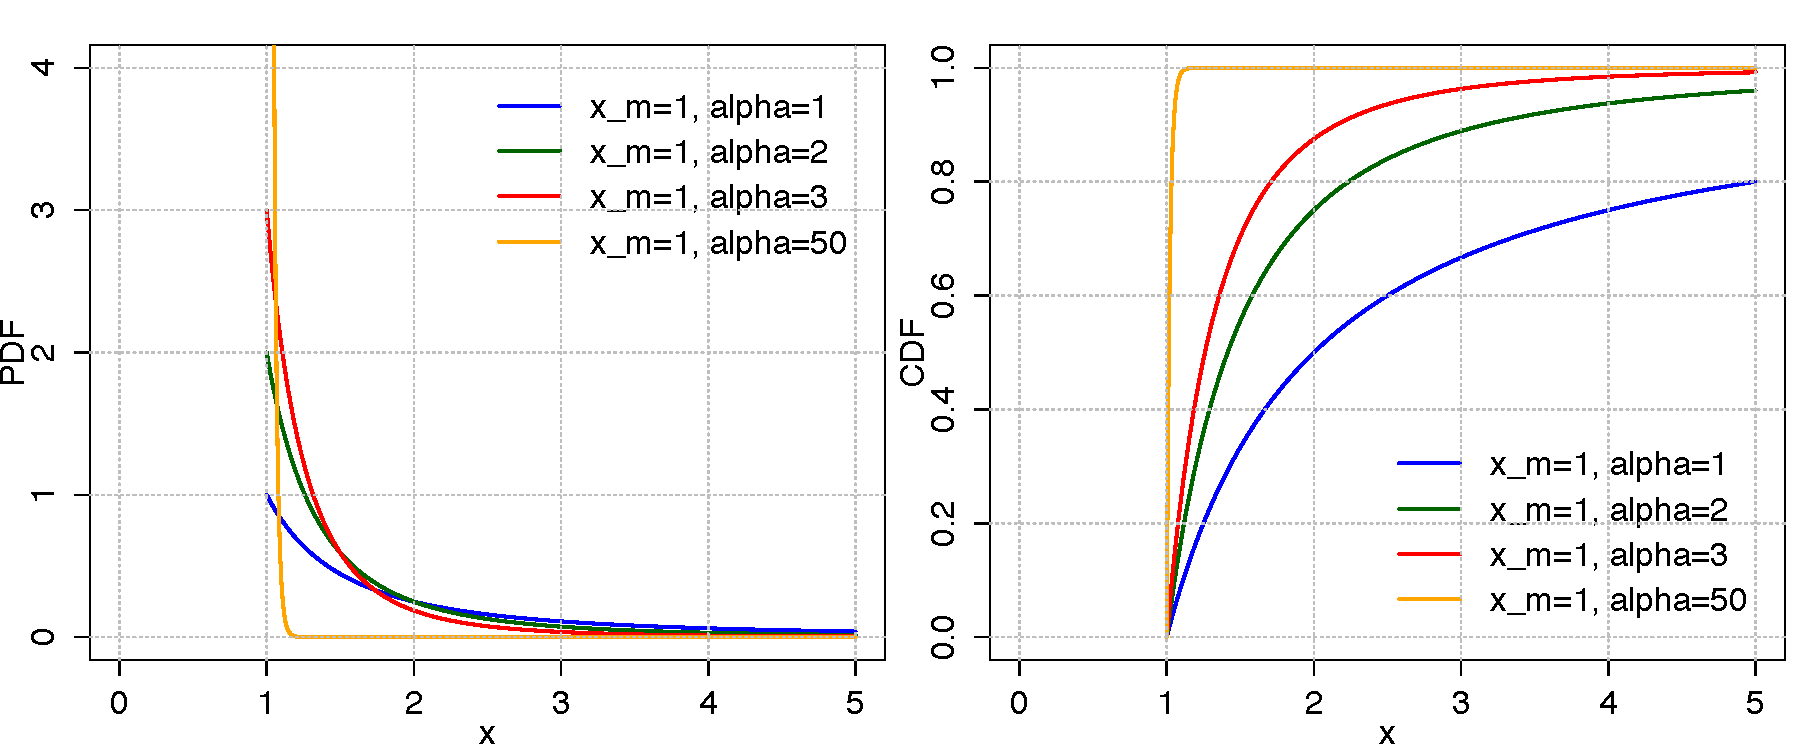
\includegraphics[width=140mm]{pics/Pareto_pdf_cdf.pdf}
 \caption{PDF and CDF of the Pareto distribution plotted using the provided R-code.}
 \label{fig:Pareto_pdf_cdf}
\end{figure}


Noncentral Chi-Square Distribution\\
Noncentral F Distribution\\
Noncentral t Distribution\\

\subsubsection*{Parameter: scale}

\noindent\begin{tabular}{p{2cm}cl}
\textbf{name} & & scale \\
\textbf{type} & & scalar \\
\textbf{symbol} & & $x_m$  \\
\textbf{definition} & & $x_m > 0, x_m \in R$
\end{tabular}
\subsubsection*{Parameter: shape}

\noindent\begin{tabular}{p{2cm}cl}
\textbf{name} & & shape \\
\textbf{type} & & scalar \\
\textbf{symbol} & & $\alpha$  \\
\textbf{definition} & & $\alpha > 0, \alpha \in R$
\end{tabular}
\subsubsection*{Functions}

\smallskip \noindent \hspace{.2cm} \textbf{PDF} 
\begin{equation*}\frac{\alpha\,x_m^\alpha}{x^{\alpha+1}}\text{ for }x\ge x_m\end{equation*}
\smallskip \noindent \hspace{.2cm} \textbf{PDF in R}  
\begin{verbatim}(alpha * x_m^alpha) / x^(alpha+1)\end{verbatim}
\smallskip \noindent \hspace{.2cm} \textbf{CDF} 
\begin{equation*}1-\left(\frac{x_m}{x}\right)^\alpha \text{ for } x \ge x_m\end{equation*}
\smallskip \noindent \hspace{.2cm} \textbf{CDF in R}  
\begin{verbatim}1-(x_m/x)^alpha\end{verbatim}
\smallskip\section*{Poisson} 

  \bigskip 

\begin{tabular}{p{2cm}cl}
\textbf{name} & & Poisson (ID: 0000187)\\ 
 
\textbf{type} & & discrete \\ 

\textbf{variate} & & $k$, scalar \\ 

\textbf{support} & & $k \in \{0,1,2,3,\dots\}$
\end{tabular}
\subsubsection*{Parameter: rate}

\noindent\begin{tabular}{p{2cm}cl}
\textbf{name} & & Poisson intensity \\
\textbf{type} & & scalar \\
\textbf{symbol} & & $\lambda$  \\
\textbf{definition} & & $\lambda \in R, \lambda > 0$
\end{tabular}

\begin{figure}[htb!]
\centering
  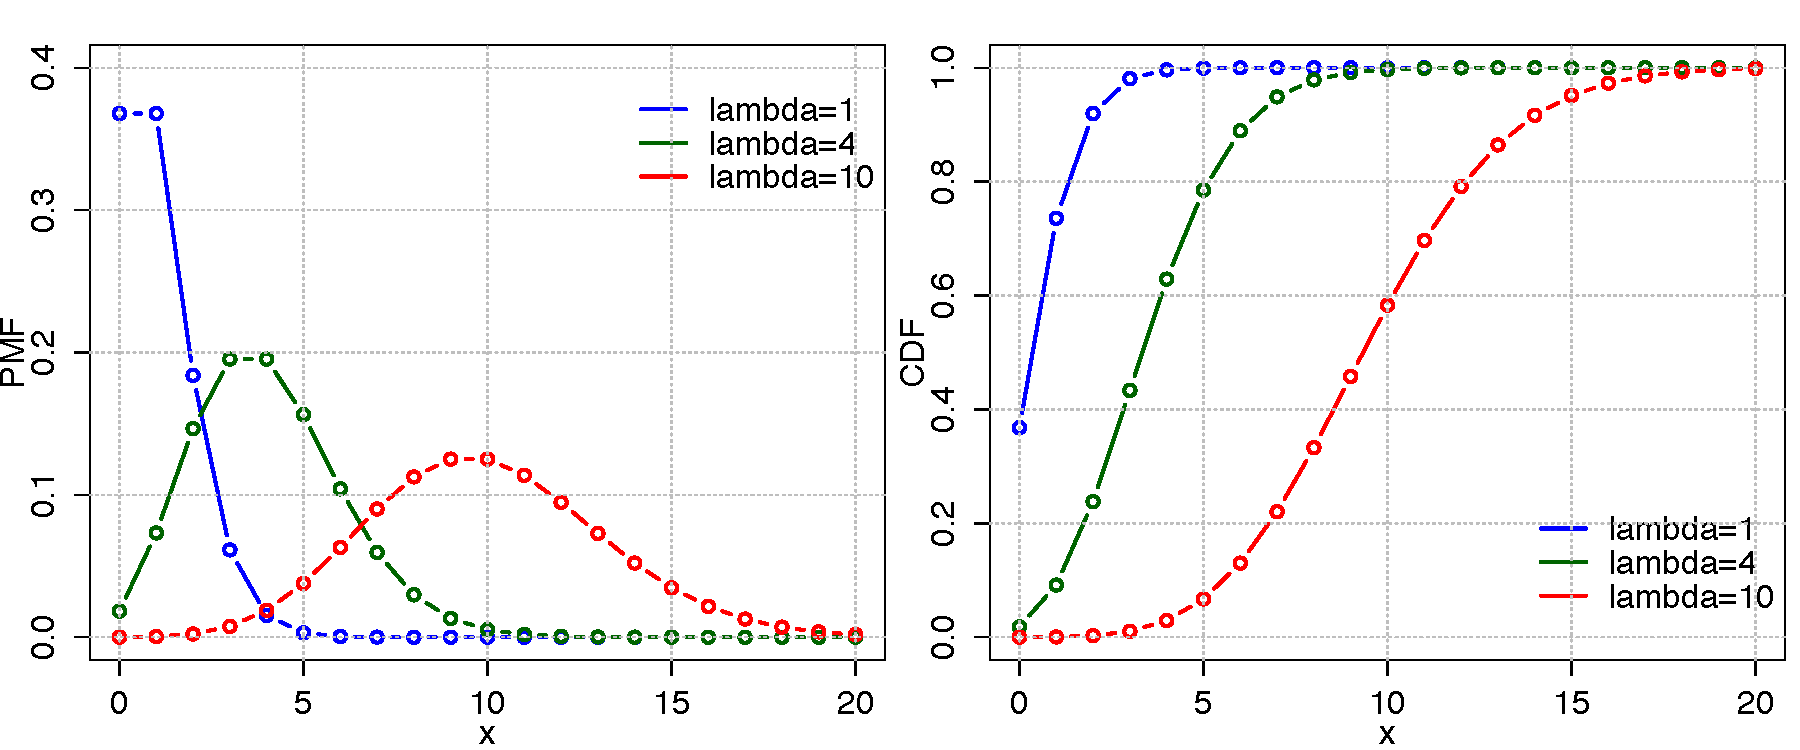
\includegraphics[width=140mm]{pics/Poisson_pmf_cdf.pdf}
 \caption{PMF and CDF of the Poisson distribution plotted using the provided R-code.}
 \label{fig:Poissonpmfcdf}
\end{figure}

\subsubsection*{Functions}

\smallskip \noindent \hspace{.2cm} \textbf{PMF} 
\begin{equation*}\frac{\lambda^k}{k!}e^{-\lambda}\end{equation*}
\smallskip \noindent \hspace{.2cm} \textbf{PMF in R}  
\begin{verbatim}lambda^k/factorial(k) * exp(-lambda)\end{verbatim}
\smallskip \noindent \hspace{.2cm} \textbf{CDF} 
\begin{equation*}\frac{\gamma(\lfloor k+1 \rfloor,\lambda)}{\lfloor k \rfloor!}\end{equation*}
\smallskip \noindent \hspace{.2cm} \textbf{CDF in R} 
\begin{verbatim}Igamma(floor(k+1), lambda, lower=F) / factorial(floor(k))\end{verbatim}
\smallskip\section*{Rayleigh} 

  \bigskip 

\begin{tabular}{p{2cm}cl}
\textbf{name} & & Rayleigh (ID: 0000197)\\ 
 
\textbf{type} & & continuous \\ 

\textbf{variate} & & $x$, scalar \\ 

\textbf{support} & & $x \in [0,+\infty)$
\end{tabular}
\subsubsection*{Parameter: scale}

\noindent\begin{tabular}{p{2cm}cl}
\textbf{name} & & scale \\
\textbf{type} & & scalar \\
\textbf{symbol} & & $\sigma$  \\
\textbf{definition} & & $\sigma > 0$
\end{tabular}

\begin{figure}[htb!]
\centering
  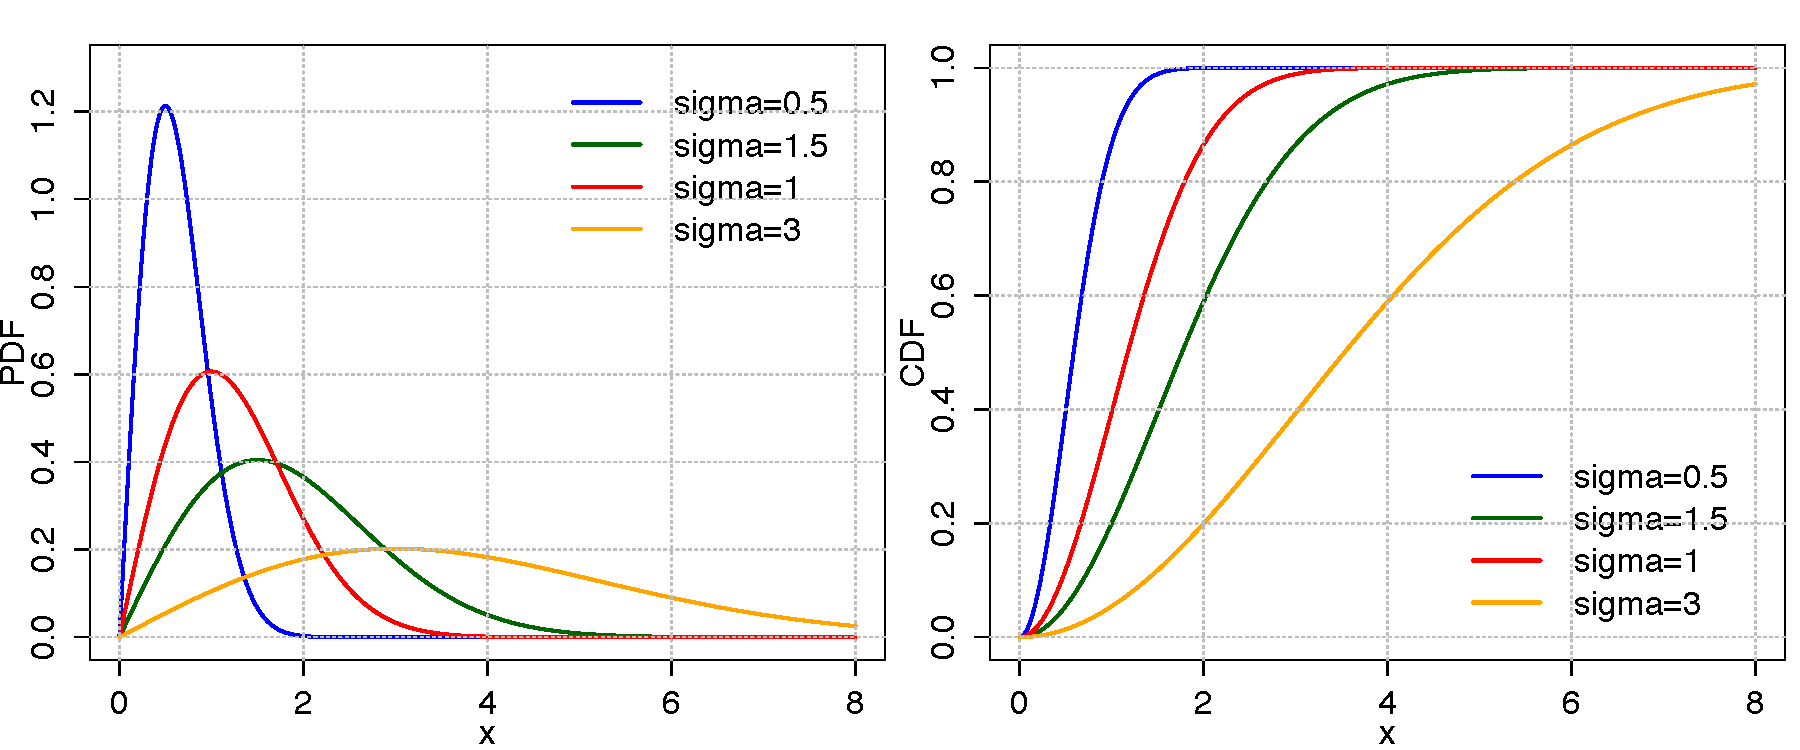
\includegraphics[width=140mm]{pics/Rayleigh_pdf_cdf.pdf}
 \caption{PDF and CDF of the Rayleigh distribution plotted using the provided R-code.}
 \label{fig:Rayleigh_pdf_cdf}
\end{figure}

\subsubsection*{Functions}

\smallskip \noindent \hspace{.2cm} \textbf{PDF} 
\begin{equation*}\frac{x}{\sigma^2} e^{-x^2/2\sigma^2}\end{equation*}
\smallskip \noindent \hspace{.2cm} \textbf{CDF} 
\begin{equation*}1 - e^{-x^2/2\sigma^2}\end{equation*}
\smallskip\section*{StandardNormal} 

  \bigskip 

\begin{tabular}{p{2cm}cl}
\textbf{name} & & Standard Normal (ID: 0000206)\\ 
 
\textbf{type} & & continuous \\ 

\textbf{variate} & & $x$, scalar \\ 

\textbf{support} & & $x \in R$
\end{tabular}
\subsubsection*{Parameter: mean}

\noindent\begin{tabular}{p{2cm}cl}
\textbf{name} & & mean \\
\textbf{type} & & scalar \\
\textbf{symbol} & & $\mu$  \\
\textbf{definition} & & $\mu=0$
\end{tabular}
\subsubsection*{Parameter: stdev}

\noindent\begin{tabular}{p{2cm}cl}
\textbf{name} & & standard deviation \\
\textbf{type} & & scalar \\
\textbf{symbol} & & $\sigma$  \\
\textbf{definition} & & $\sigma=1$
\end{tabular}

\begin{figure}[htb!]
\centering
  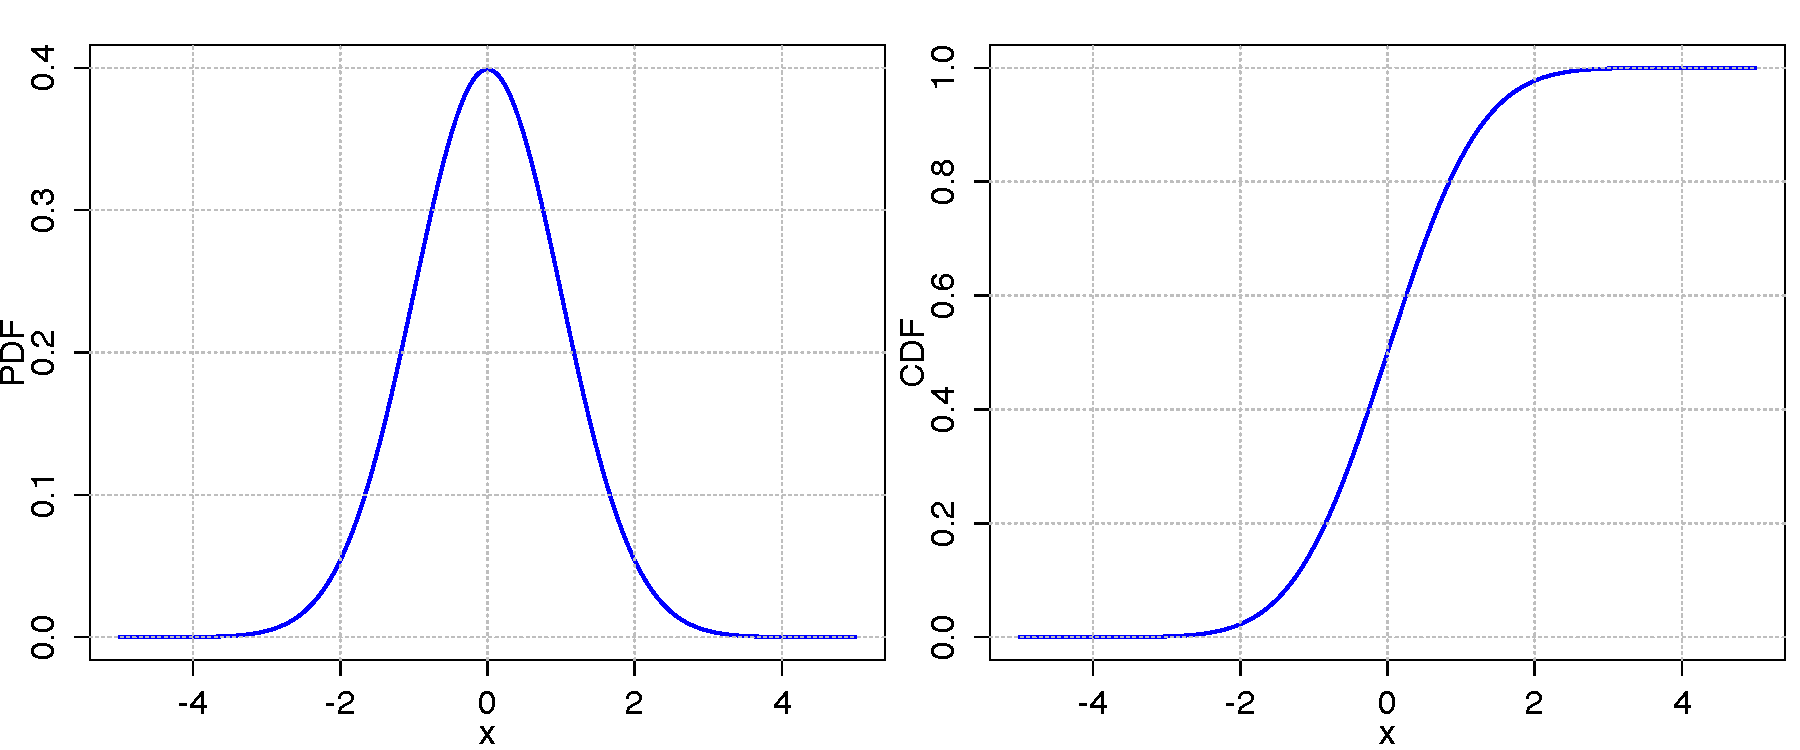
\includegraphics[width=140mm]{pics/StandardNormal_pdf_cdf.pdf}
 \caption{PDF and CDF of the Standard Normal distribution plotted using the provided R-code.}
 \label{fig:StandardNormalpdfcdf}
\end{figure}

\subsubsection*{Functions}

\smallskip \noindent \hspace{.2cm} \textbf{PDF} 
\begin{equation*}\frac{e^{-\frac{1}{2} x^2}}{\sqrt{2\pi}}\end{equation*}
\smallskip \noindent \hspace{.2cm} \textbf{PDF in R}  
\begin{verbatim}1/(sqrt(2*pi))*exp(-x^2/2)\end{verbatim}
\smallskip \noindent \hspace{.2cm} \textbf{CDF} 
\begin{equation*}\frac12\left[1 + \text{erf}\left( \frac{x}{\sqrt{2}}\right)\right]\end{equation*}
\smallskip \noindent \hspace{.2cm} \textbf{CDF in R} 
\begin{verbatim}1/2 * (1 + erf(x/(sqrt(2))))\end{verbatim}
\smallskip\section*{StandardUniform} 

  \bigskip 

\begin{tabular}{p{2cm}cl}
\textbf{name} & & Standard Uniform (ID: 0000225)\\ 
 
\textbf{type} & & continuous \\ 

\textbf{variate} & & $x$, scalar \\ 

\textbf{support} & & $x \in [0,1]$
\end{tabular}
\subsubsection*{Parameter: minimum}

\noindent\begin{tabular}{p{2cm}cl}
\textbf{name} & & minimum \\
\textbf{type} & & scalar \\
\textbf{symbol} & & $a$  \\
\textbf{definition} & & $a=0$
\end{tabular}

\begin{figure}[htb!]
\centering
  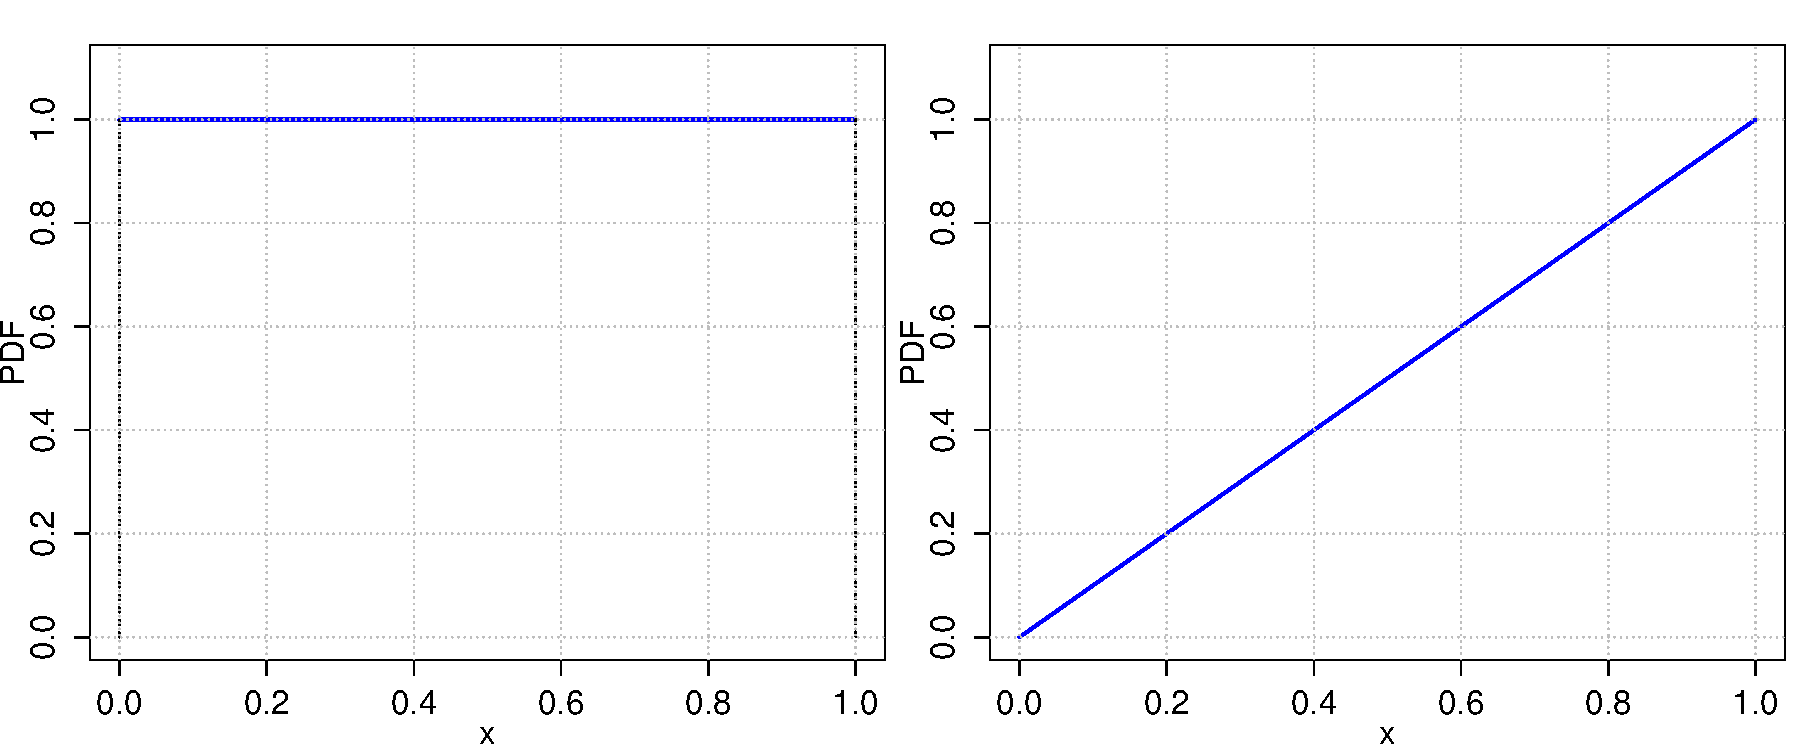
\includegraphics[width=140mm]{pics/StandardUniform_pdf_cdf}
 \caption{PDF and CDF of the Standard Uniform distribution plotted using the provided R-code.}
 \label{fig:StandardUniformpdfcdf}
\end{figure}

\subsubsection*{Parameter: maximum}

\noindent\begin{tabular}{p{2cm}cl}
\textbf{name} & & maximum \\
\textbf{type} & & scalar \\
\textbf{symbol} & & $b$  \\
\textbf{definition} & & $b=1$
\end{tabular}
\subsubsection*{Functions}

\smallskip \noindent \hspace{.2cm} \textbf{PDF} 
\begin{equation*}1\end{equation*}
\smallskip \noindent \hspace{.2cm} \textbf{PDF in R}  
\begin{verbatim}1\end{verbatim}
\smallskip \noindent \hspace{.2cm} \textbf{CDF} 
\begin{equation*}x\end{equation*}
\smallskip \noindent \hspace{.2cm} \textbf{CDF in R} 
\begin{verbatim}x\end{verbatim}
\smallskip\section*{StudentT} 

  \bigskip 

\begin{tabular}{p{2cm}cl}
\textbf{name} & & Student's t-distribution (ID: 0000216)\\ 
 
\textbf{type} & & continuous \\ 

\textbf{variate} & & $x$, scalar \\ 

\textbf{support} & & $x \in (-\infty,+\infty)$
\end{tabular}
\subsubsection*{Parameter: degreesOfFreedom}

\noindent\begin{tabular}{p{2cm}cl}
\textbf{name} & & degrees of freedom \\
\textbf{type} & & scalar \\
\textbf{symbol} & & $\nu$  \\
\textbf{definition} & & $\nu > 0, \nu \in  R$
\end{tabular}

\begin{figure}[htb!]
\centering
  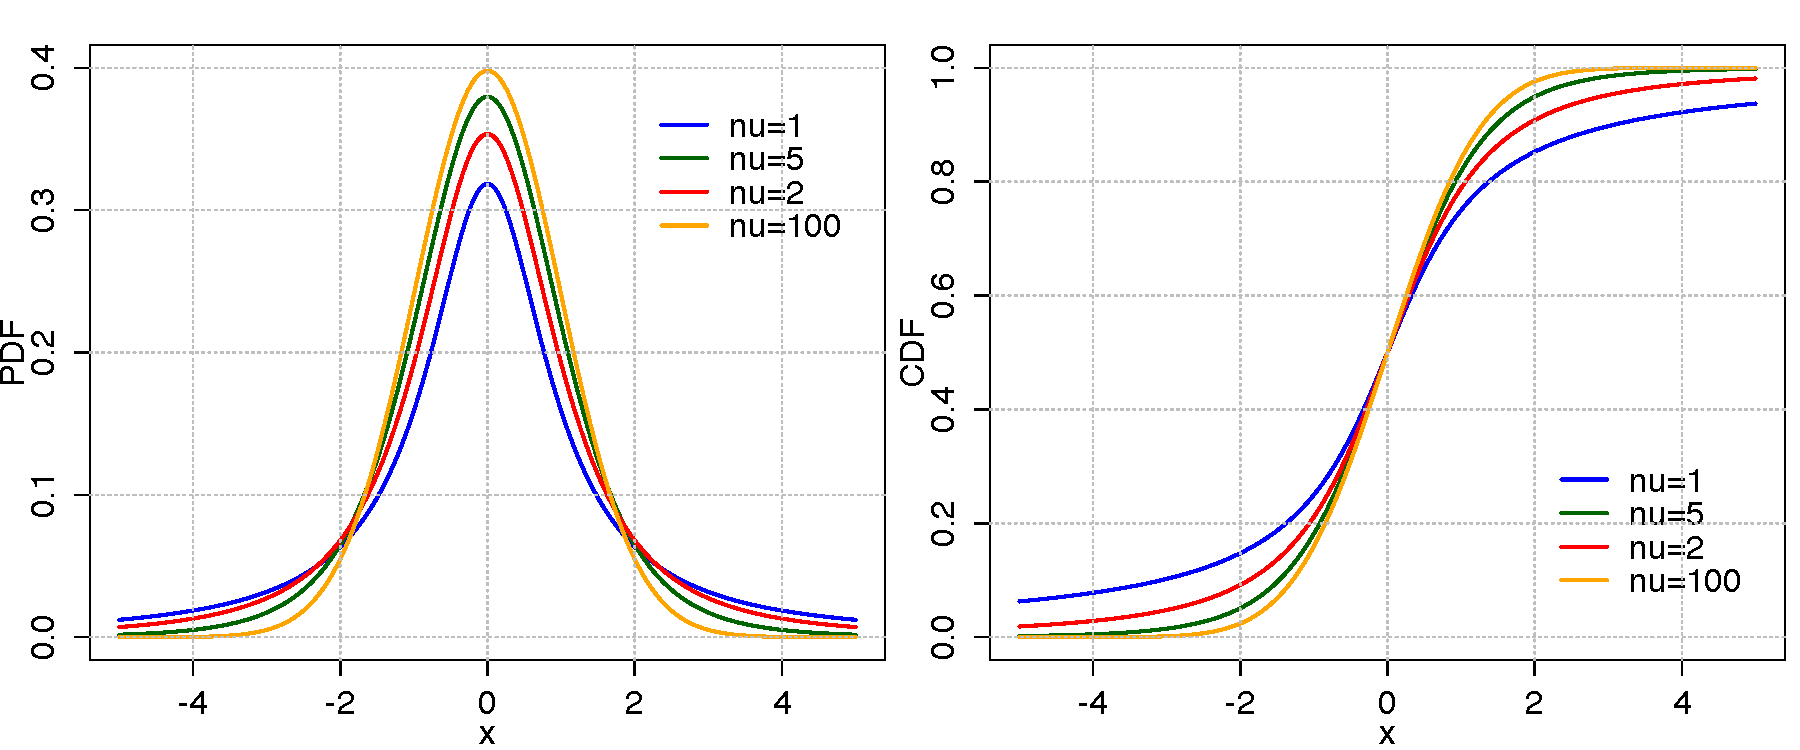
\includegraphics[width=140mm]{pics/StudentT_pdf_cdf.pdf}
 \caption{PDF and CDF of the StudentT distribution plotted using the provided R-code.}
 \label{fig:StudentTpdfcdf}
\end{figure}

\subsubsection*{Functions}

\smallskip \noindent \hspace{.2cm} \textbf{PDF} 
\begin{equation*}\frac{\Gamma \left(\frac{\nu+1}{2} \right)} {\sqrt{\nu\pi}\,\Gamma \left(\frac{\nu}{2} \right)} \left(1+\frac{x^2}{\nu} \right)^{-\frac{\nu+1}{2}}\end{equation*}
\smallskip \noindent \hspace{.2cm} \textbf{PDF in R}  
\begin{verbatim}gamma((nu+1)/2)/(sqrt(nu*pi)*gamma(nu/2))*(1+x^2/nu)^(-(nu+1)/2)\end{verbatim}
\smallskip \noindent \hspace{.2cm} \textbf{CDF} 
\begin{equation*}\begin{matrix}
     \frac{1}{2} + x \Gamma \left( \frac{\nu+1}{2} \right)  \times
     \frac{\,_2F_1 \left ( \frac{1}{2},\frac{\nu+1}{2};\frac{3}{2};
           -\frac{x^2}{\nu} \right)}
     {\sqrt{\pi\nu}\,\Gamma \left(\frac{\nu}{2}\right)}
     \end{matrix}\end{equation*}
\smallskip \noindent \hspace{.2cm} \textbf{CDF in R} 
\begin{verbatim}1/2+x*gamma((nu+1)/2)*hypergeo(1/2,(nu+1)/2,3/2,-x^2/nu)/( sqrt(pi*nu) *gamma(nu/2))\end{verbatim}
\smallskip\section*{Triangular} 

  \bigskip 

\begin{tabular}{p{2cm}cl}
\textbf{name} & & Triangular (ID: 0000235)\\ 
 
\textbf{type} & & continuous \\ 

\textbf{variate} & & $x$, scalar \\ 

\textbf{support} & & $a \leq x \leq b$
\end{tabular}

\begin{figure}[htb!]
\centering
  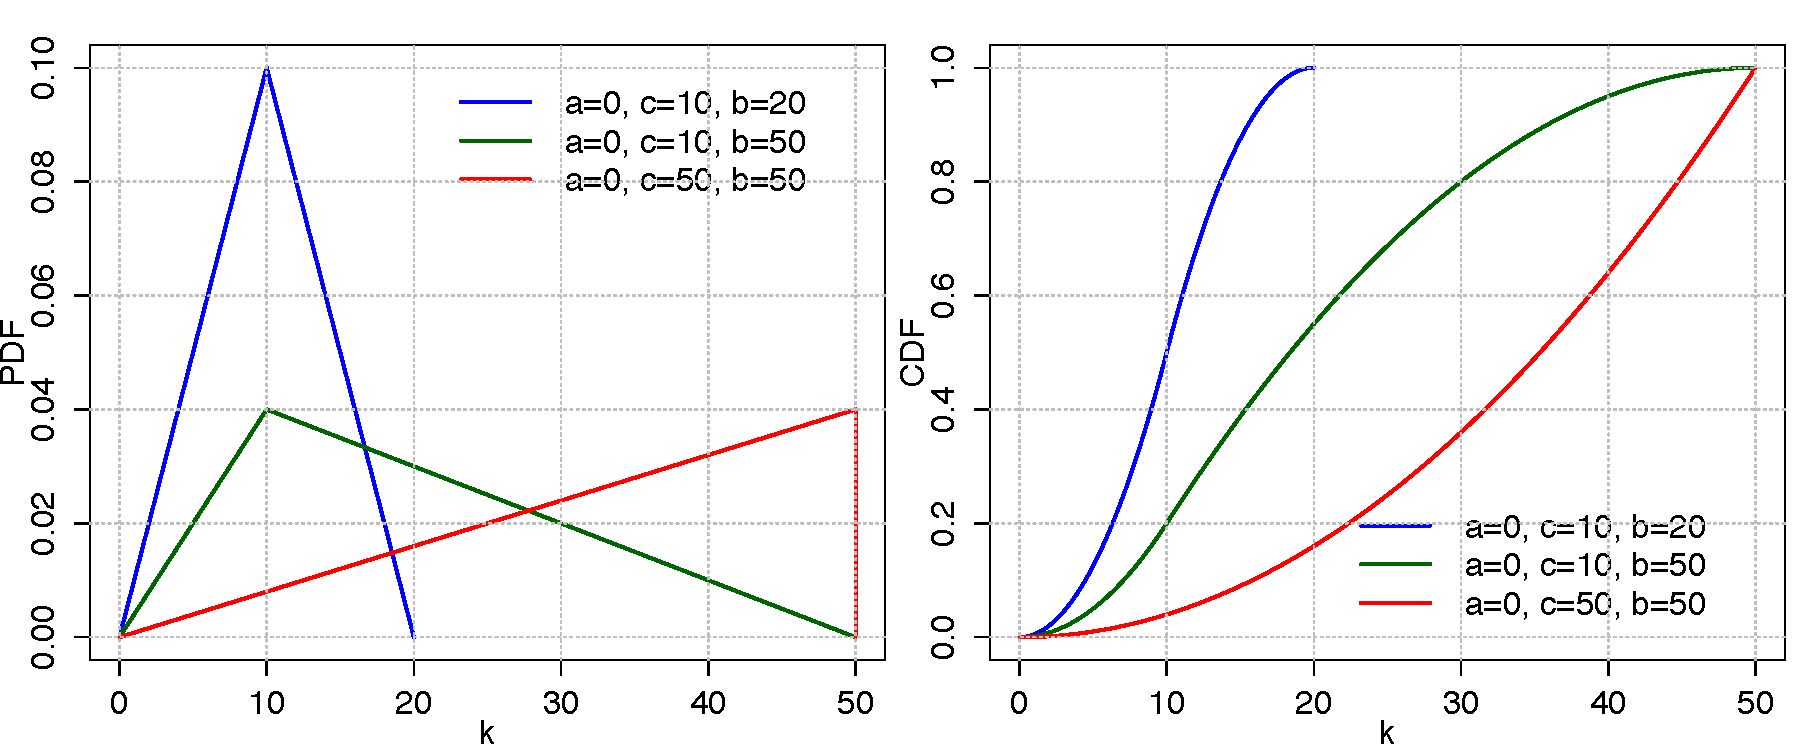
\includegraphics[width=140mm]{pics/Triangular_pmf_cdf.pdf}
 \caption{PDF and CDF of the Triangular distribution plotted using the provided R-code.}
 \label{fig:Triangular_pmf_cdf}
\end{figure}

\subsubsection*{Parameter: lowerLimit}

\noindent\begin{tabular}{p{2cm}cl}
\textbf{name} & & lower limit \\
\textbf{type} & & scalar \\
\textbf{symbol} & & $a$  \\
\textbf{definition} & & $a \in R$
\end{tabular}
\subsubsection*{Parameter: upperLimit}

\noindent\begin{tabular}{p{2cm}cl}
\textbf{name} & & upper limit \\
\textbf{type} & & scalar \\
\textbf{symbol} & & $b$  \\
\textbf{definition} & & $b \in R, a < b$
\end{tabular}
\subsubsection*{Parameter: shape}

\noindent\begin{tabular}{p{2cm}cl}
\textbf{name} & & shape (mode) \\
\textbf{type} & & scalar \\
\textbf{symbol} & & $c$  \\
\textbf{definition} & & $c \in R$
\end{tabular}
\subsubsection*{Functions}

\smallskip \noindent \hspace{.2cm} \textbf{PDF} 
\begin{equation*}\begin{cases}
2(x-a) / [(b-a)(c-a)] & \text{ for } a \leq x \leq c \\
2(b-x) / [(b-a)(b-c)] & \text{ for } c \leq x \leq b
\end{cases}\end{equation*}
\smallskip \noindent \hspace{.2cm} \textbf{PDF in R}  
\begin{verbatim}2*(x-a) / ((b-a)*(c-a)) for a <= x <= c \\
2*(b-x) / ((b-a)*(b-c)) for c <= x <= b \end{verbatim}
\smallskip \noindent \hspace{.2cm} \textbf{CDF} 
\begin{equation*}\begin{cases}
(x-a)^2 / [(b-a)(c-a)] & \text{ for } a \leq x \leq c \\
1 - (b-x)^2 / [(b-a)(b-c)] & \text{ for } c \leq x \leq b
\end{cases}\end{equation*}
\smallskip \noindent \hspace{.2cm} \textbf{CDF in R} 
\begin{verbatim}(x-a)^2 / ((b-a)*(c-a)) for a <= x <= c \\
1 - (b-x)^2 / ((b-a)*(b-c)) for c <= x <= b \end{verbatim}
\smallskip\section*{TruncatedNormal} 

  \bigskip 

\begin{tabular}{p{2cm}cl}
\textbf{name} & & Truncated Normal (ID: 0000246)\\ 
 
\textbf{type} & & continuous \\ 

\textbf{variate} & & $x$, scalar \\ 

\textbf{support} & & $x \in [a,b]$
\end{tabular}

\begin{figure}[htb!]
\centering
  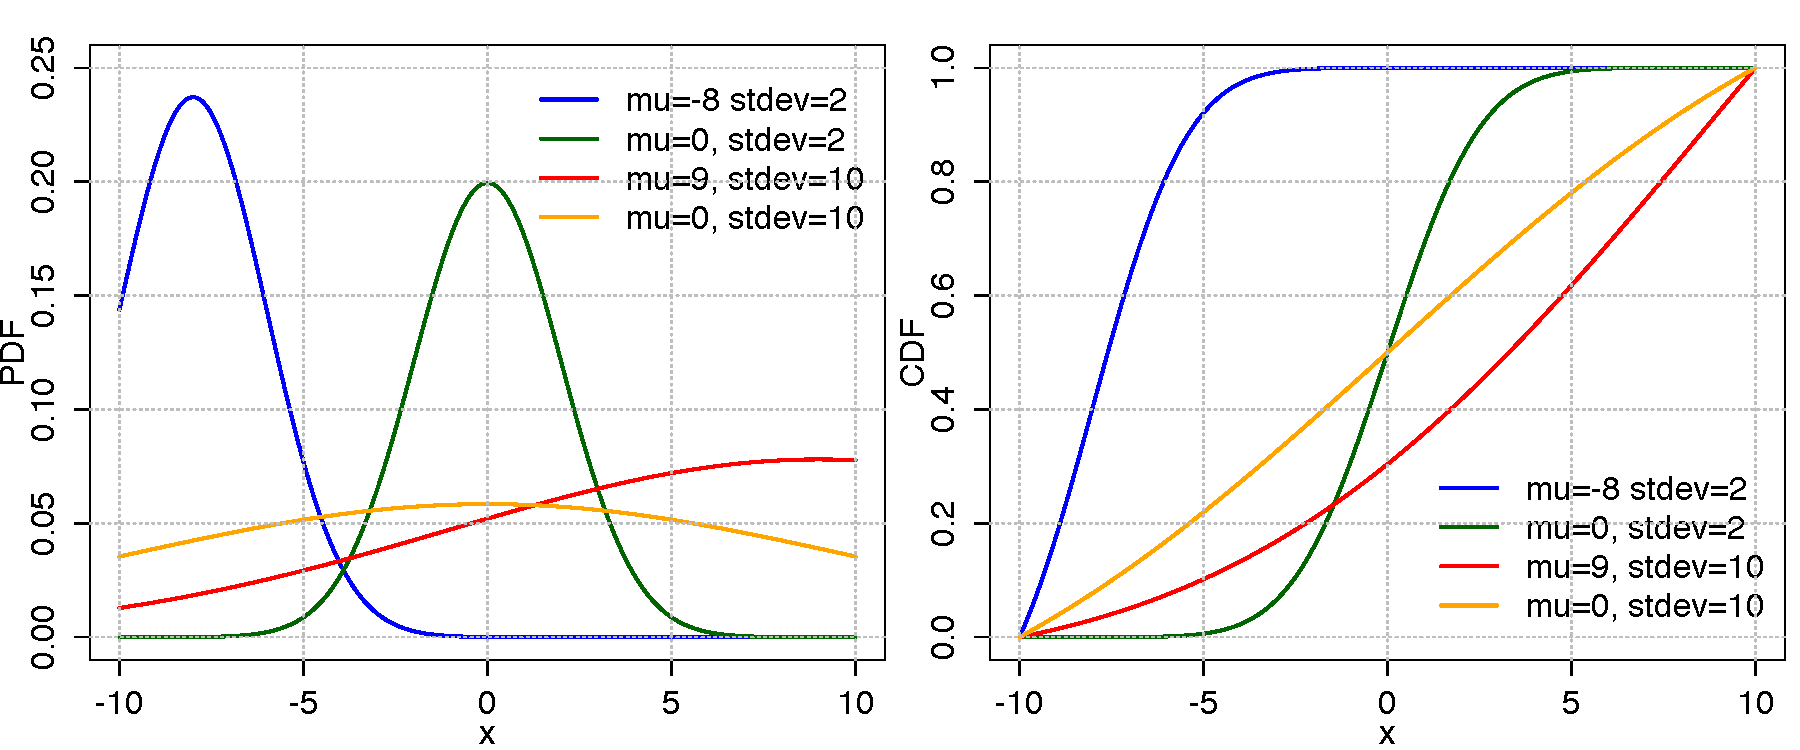
\includegraphics[width=140mm]{pics/TruncatedNormal_pdf_cdf.pdf}
 \caption{PDF and CDF of the Truncated Normal distribution plotted using the provided R-code.}
 \label{fig:TruncatedNormal_pdf_cdf}
\end{figure}

\subsubsection*{Parameter: mean}

\noindent\begin{tabular}{p{2cm}cl}
\textbf{name} & & mean \\
\textbf{type} & & scalar \\
\textbf{symbol} & & $\mu$  \\
\textbf{definition} & & $\mu \in R$
\end{tabular}
\subsubsection*{Parameter: stdev}

\noindent\begin{tabular}{p{2cm}cl}
\textbf{name} & & standard deviation \\
\textbf{type} & & scalar \\
\textbf{symbol} & & $\sigma$  \\
\textbf{definition} & & $\sigma > 0$
\end{tabular}
\subsubsection*{Parameter: lowerBound}

\noindent\begin{tabular}{p{2cm}cl}
\textbf{name} & & lower bound \\
\textbf{type} & & scalar \\
\textbf{symbol} & & $a$  \\
\textbf{definition} & & $a \in R$
\end{tabular}
\subsubsection*{Parameter: upperBound}

\noindent\begin{tabular}{p{2cm}cl}
\textbf{name} & & upper bound \\
\textbf{type} & & scalar \\
\textbf{symbol} & & $b$  \\
\textbf{definition} & & $b \in R, b > a$
\end{tabular}
\subsubsection*{Functions}

\smallskip \noindent \hspace{.2cm} \textbf{PDF} 
\begin{equation*}\frac{\frac{1}{\sigma} \phi(\frac{x-\mu}{\sigma})}{\Phi(\frac{b-\mu}{\sigma})-\Phi(\frac{a-\mu}{\sigma})}\end{equation*}
\smallskip \noindent \hspace{.2cm} \textbf{PDF in R}  
\begin{verbatim}( 1/sigma * phi((x-mu)/sigma) ) / ( Phi((b-mu)/sigma)-Phi((a-mu)/sigma) )\end{verbatim}
\smallskip \noindent \hspace{.2cm} \textbf{CDF} 
\begin{equation*}\frac{\Phi(\frac{x-\mu}{\sigma})-\Phi(\frac{a-\mu}{\sigma})}{\Phi(\frac{b-\mu}{\sigma})-\Phi(\frac{a-\mu}{\sigma})}\end{equation*}
\smallskip \noindent \hspace{.2cm} \textbf{CDF in R} 
\begin{verbatim}( Phi((x-mu)/sigma)-Phi((a-mu)/sigma) ) / ( Phi((b-mu)/sigma)-Phi((a-mu)/sigma) )\end{verbatim}
\smallskip\section*{Uniform} 

  \bigskip 

\begin{tabular}{p{2cm}cl}
\textbf{name} & & Uniform (ID: 0000258)\\ 
 
\textbf{type} & & continuous \\ 

\textbf{variate} & & $x$, scalar \\ 

\textbf{support} & & $x \in [a,b]$
\end{tabular}

\begin{figure}[htb!]
\centering
  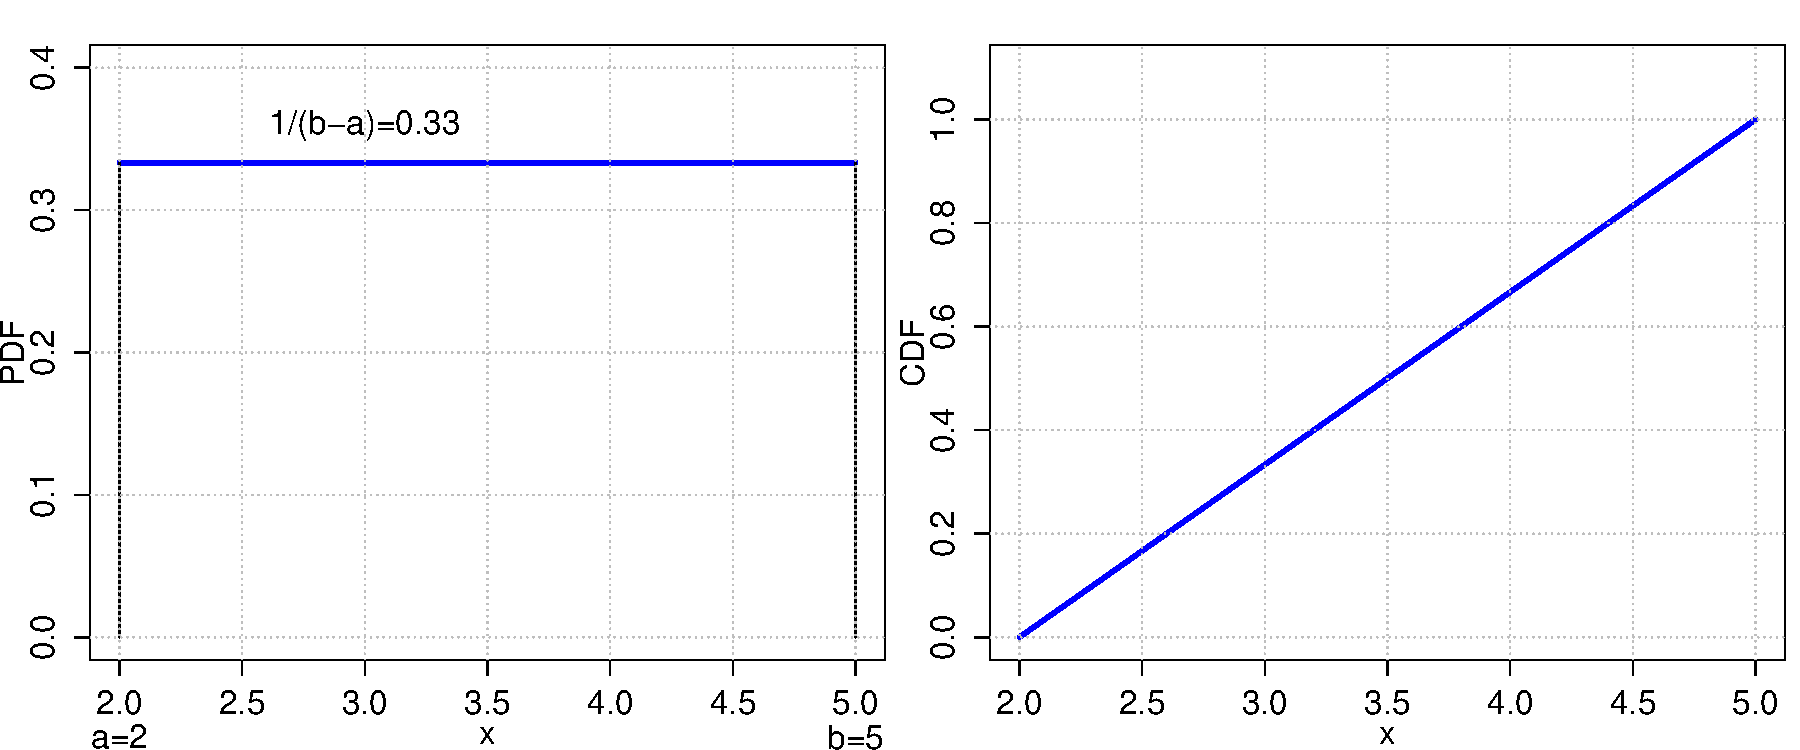
\includegraphics[width=140mm]{pics/Uniform_pdf_cdf.pdf}
 \caption{PDF and CDF of the Uniform distribution plotted using the provided R-code.}
 \label{fig:Uniformpdfcdf}
\end{figure}

\subsubsection*{Parameter: minimum}

\noindent\begin{tabular}{p{2cm}cl}
\textbf{name} & & minimum \\
\textbf{type} & & scalar \\
\textbf{symbol} & & $a$  \\
\textbf{definition} & & $a \in  R$
\end{tabular}
\subsubsection*{Parameter: maximum}

\noindent\begin{tabular}{p{2cm}cl}
\textbf{name} & & maximum \\
\textbf{type} & & scalar \\
\textbf{symbol} & & $b$  \\
\textbf{definition} & & $b \in R, a < b$
\end{tabular}
\subsubsection*{Functions}

\smallskip \noindent \hspace{.2cm} \textbf{PDF} 
\begin{equation*}\begin{cases}
                  \frac{1}{b - a} & \text{for } x \in [a,b]  \\
                  0               & \text{otherwise}
                \end{cases}\end{equation*}
\smallskip \noindent \hspace{.2cm} \textbf{PDF in R}  
\begin{verbatim}1/(b-a)\end{verbatim}
\smallskip \noindent \hspace{.2cm} \textbf{CDF} 
\begin{equation*}\begin{cases}
                  0               & \text{for } x < a \\
                  \frac{x-a}{b-a} & \text{for } x \in [a,b) \\
                  1               & \text{for } x \ge b
                \end{cases}\end{equation*}
\smallskip \noindent \hspace{.2cm} \textbf{CDF in R} 
\begin{verbatim}(x-a)/(b-a)\end{verbatim}
\smallskip\section*{UniformDiscrete1} 

  \bigskip 

\begin{tabular}{p{2cm}cl}
\textbf{name} & & Uniform Discrete 1 (ID: 0000268)\\ 
 
\textbf{type} & & discrete \\ 

\textbf{variate} & & $x$, scalar \\ 

\textbf{support} & & $a,b \in \{\dots,-2,-1,0,1,2,3,\dots\}$
\end{tabular}
\subsubsection*{Parameter: minimum}

\noindent\begin{tabular}{p{2cm}cl}
\textbf{name} & & minimum \\
\textbf{type} & & scalar \\
\textbf{symbol} & & $a$  \\
\textbf{definition} & & $a \in \{\dots,-2,-1,0,1,2,3,\dots\}$
\end{tabular}
\subsubsection*{Parameter: maximum}

\noindent\begin{tabular}{p{2cm}cl}
\textbf{name} & & maximum \\
\textbf{type} & & scalar \\
\textbf{symbol} & & $b$  \\
\textbf{definition} & & $b \in \{\dots,-2,-1,0,1,2,3,\dots\}, b \ge a$
\end{tabular}
\subsubsection*{Parameter: numberOfValues}

\noindent\begin{tabular}{p{2cm}cl}
\textbf{name} & & number of values \\
\textbf{type} & & scalar \\
\textbf{symbol} & & $n$  \\
\textbf{definition} & & $n=b-a+1$
\end{tabular}
\subsubsection*{Functions}

\smallskip \noindent \hspace{.2cm} \textbf{PMF} 
\begin{equation*}1/n\end{equation*}
\smallskip \noindent \hspace{.2cm} \textbf{CDF} 
\begin{equation*}\frac{\lfloor k \rfloor -a+1}{n}\end{equation*}
\smallskip\section*{UniformDiscrete2} 

  \bigskip 

\begin{tabular}{p{2cm}cl}
\textbf{name} & & Uniform Discrete 2 (ID: 0000279)\\ 
 
\textbf{type} & & discrete \\ 

\textbf{variate} & & $x$, scalar \\ 

\textbf{support} & & $x \in \{0,1,2,\dots,n\}$
\end{tabular}
\subsubsection*{Parameter: minimum}

\noindent\begin{tabular}{p{2cm}cl}
\textbf{name} & & minimum \\
\textbf{type} & & scalar \\
\textbf{symbol} & & $a$  \\
\textbf{definition} & & $a=0$
\end{tabular}
\subsubsection*{Parameter: numberOfValues}

\noindent\begin{tabular}{p{2cm}cl}
\textbf{name} & & number of values \\
\textbf{type} & & scalar \\
\textbf{symbol} & & $n$  \\
\textbf{definition} & & $n \in N$
\end{tabular}
\subsubsection*{Functions}

\smallskip \noindent \hspace{.2cm} \textbf{PMF} 
\begin{equation*}1/(n+1)\end{equation*}
\smallskip \noindent \hspace{.2cm} \textbf{CDF} 
\begin{equation*}\frac{x+1}{n+1}\end{equation*}
\smallskip\section*{Weibull1} 

  \bigskip 

\begin{tabular}{p{2cm}cl}
\textbf{name} & & Weibull 1 (ID: 0000289)\\ 
 
\textbf{type} & & continuous \\ 

\textbf{variate} & & $x$, scalar \\ 

\textbf{support} & & $x \in [0,+\infty)$
\end{tabular}
\subsubsection*{Parameter: scale}

\noindent\begin{tabular}{p{2cm}cl}
\textbf{name} & & scale \\
\textbf{type} & & scalar \\
\textbf{symbol} & & $\lambda$  \\
\textbf{definition} & & $\lambda\in (0, +\infty)$
\end{tabular}

\begin{figure}[htb!]
\centering
  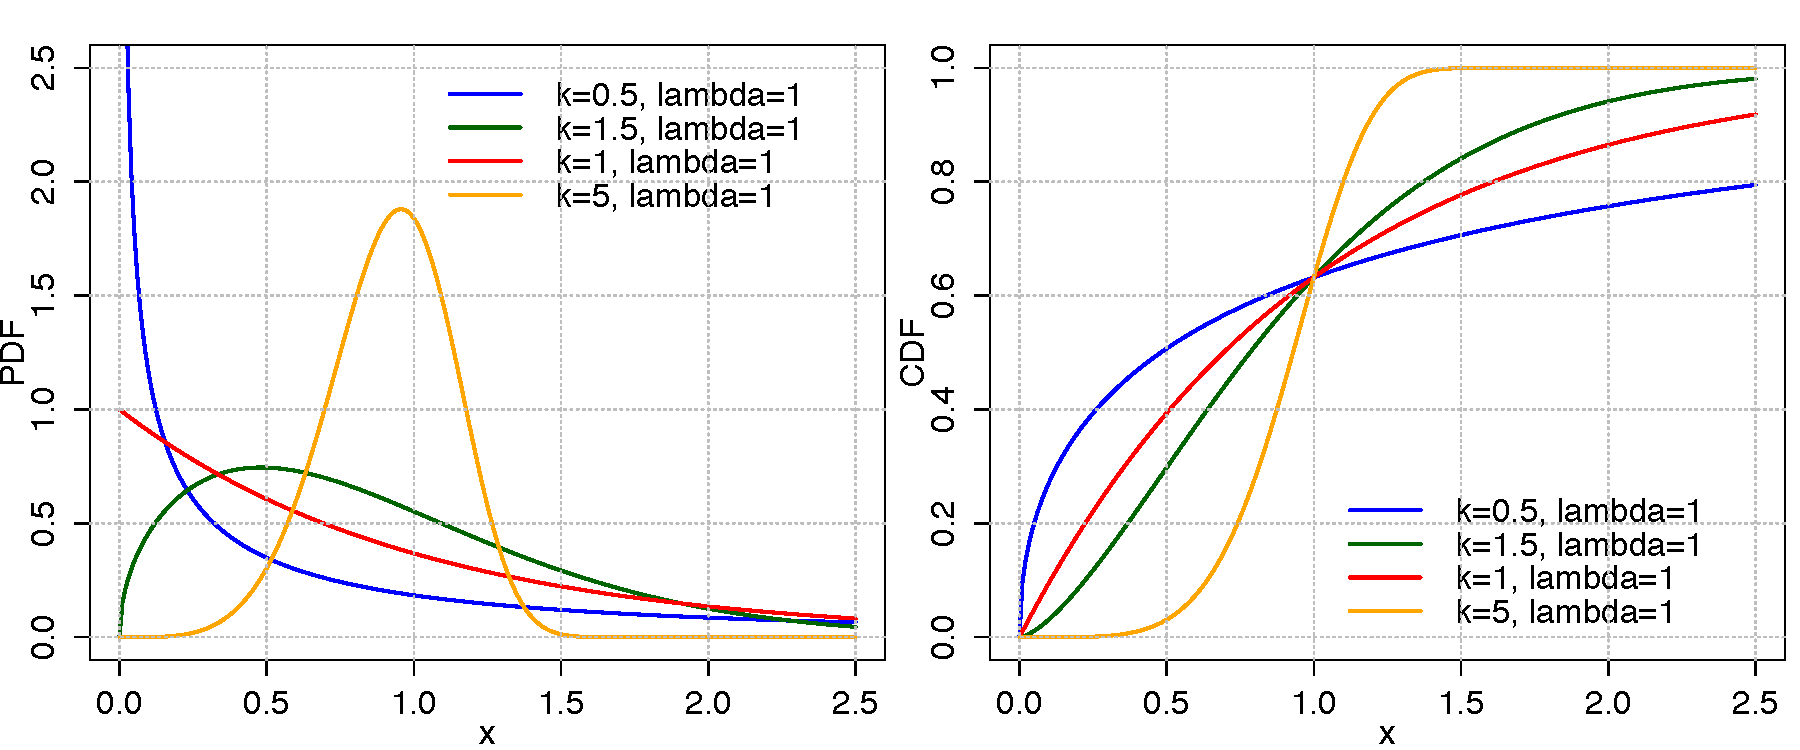
\includegraphics[width=140mm]{pics/Weibull1_pdf_cdf.pdf}
 \caption{PDF and CDF of the Weibull1 distribution plotted using the provided R-code.}
 \label{fig:Weibull1pdfcdf}
\end{figure}

\subsubsection*{Parameter: shape}

\noindent\begin{tabular}{p{2cm}cl}
\textbf{name} & & shape \\
\textbf{type} & & scalar \\
\textbf{symbol} & & $k$  \\
\textbf{definition} & & $k\in (0, +\infty)$
\end{tabular}
\subsubsection*{Functions}

\smallskip \noindent \hspace{.2cm} \textbf{PDF} 
\begin{equation*}\begin{cases}
\frac{k}{\lambda}\left(\frac{x}{\lambda}\right)^{k-1}e^{-(x/\lambda)^{k}} & x\geq0\\
0 & x<0\end{cases}\end{equation*}
\smallskip \noindent \hspace{.2cm} \textbf{PDF in R}  
\begin{verbatim}k/lambda * (x/lambda)^(k-1) * exp(-(x/lambda)^k)\end{verbatim}
\smallskip \noindent \hspace{.2cm} \textbf{CDF} 
\begin{equation*}\begin{cases}1- e^{-(x/\lambda)^k} & x\geq0\\ 0 & x<0\end{cases}\end{equation*}
\smallskip \noindent \hspace{.2cm} \textbf{CDF in R} 
\begin{verbatim}1- exp(-(x/lambda)^k)\end{verbatim}
\smallskip\section*{Weibull2} 

  \bigskip 

\begin{tabular}{p{2cm}cl}
\textbf{name} & & Weibull 2 (ID: 0000299)\\ 
 
\textbf{type} & & continuous \\ 

\textbf{variate} & & $x$, scalar \\ 

\textbf{support} & & $x > 0$
\end{tabular}
\subsubsection*{Parameter: lambda}

\noindent\begin{tabular}{p{2cm}cl}
\textbf{name} & & lambda \\
\textbf{type} & & scalar \\
\textbf{symbol} & & $\lambda$  \\
\textbf{definition} & & $-$
\end{tabular}
\subsubsection*{Parameter: shape}

\noindent\begin{tabular}{p{2cm}cl}
\textbf{name} & & shape \\
\textbf{type} & & scalar \\
\textbf{symbol} & & $v$  \\
\textbf{definition} & & $-$
\end{tabular}
\subsubsection*{Functions}

\smallskip \noindent \hspace{.2cm} \textbf{PDF} 
\begin{equation*}v\lambda \,x^{v-1} e^{-\lambda x^{v}}\end{equation*}
\smallskip \noindent \hspace{.2cm} \textbf{CDF} 
\begin{equation*}-\end{equation*}
\smallskip\section*{Wishart1} 

  \bigskip 

\begin{tabular}{p{2cm}cl}
\textbf{name} & & Wishart 1 (ID: 0000309)\\ 
 
\textbf{type} & & continuous \\ 

\textbf{variate} & & $X$, matrix \\ 

\textbf{support} & & $X(p \times p) - \text{positive definite matrix}$
\end{tabular}
\subsubsection*{Parameter: scaleMatrix}

\noindent\begin{tabular}{p{2cm}cl}
\textbf{name} & & scale matrix \\
\textbf{type} & & matrix \\
\textbf{symbol} & & $V$  \\
\textbf{definition} & & $V > 0, p\times p - \text{positive definite matrix}$
\end{tabular}
\subsubsection*{Parameter: degreesOfFreedom}

\noindent\begin{tabular}{p{2cm}cl}
\textbf{name} & & degrees of freedom \\
\textbf{type} & & scalar \\
\textbf{symbol} & & $n$  \\
\textbf{definition} & & $n > p-1$
\end{tabular}
\subsubsection*{Functions}

\smallskip \noindent \hspace{.2cm} \textbf{PDF} 
\begin{equation*}\frac{|X|^{\frac{n-p-1}{2}} e^{-\frac{\text{tr}(V^{-1}X)}{2}}}{2^\frac{np}{2}|V|^\frac{n}{2}\Gamma_p(\frac{n}{2})}\end{equation*}
\smallskip \noindent \hspace{.2cm} \textbf{CDF} 
\begin{equation*}-\end{equation*}
\smallskip\section*{Wishart2} 

  \bigskip 

\begin{tabular}{p{2cm}cl}
\textbf{name} & & Wishart 2 (ID: 0000319)\\ 
 
\textbf{type} & & continuous \\ 

\textbf{variate} & & $X$, matrix \\ 

\textbf{support} & & $X(p \times p) - \text{symmetric, positive definite matrix}$
\end{tabular}
\subsubsection*{Parameter: inverseScaleMatrix}

\noindent\begin{tabular}{p{2cm}cl}
\textbf{name} & & inverse scale matrix \\
\textbf{type} & & matrix \\
\textbf{symbol} & & $R$  \\
\textbf{definition} & & $p\times p - symmetric, positive definite matrix$
\end{tabular}
\subsubsection*{Parameter: degreesOfFreedom}

\noindent\begin{tabular}{p{2cm}cl}
\textbf{name} & & degrees of freedom \\
\textbf{type} & & scalar \\
\textbf{symbol} & & $k$  \\
\textbf{definition} & & $-$
\end{tabular}
\subsubsection*{Functions}

\smallskip \noindent \hspace{.2cm} \textbf{PDF} 
\begin{equation*}|R|^{k/2}|x|^{(k-p-1)/2}e^{-\frac{1}2\,tr(Rx)}\end{equation*}
\smallskip \noindent \hspace{.2cm} \textbf{CDF} 
\begin{equation*}-\end{equation*}
\smallskip\section*{ZeroInflatedNegativeBinomial} 

  \bigskip 

\begin{tabular}{p{2cm}cl}
\textbf{name} & & Zero-Inflated Negative Binomial (ID: 0000006)\\ 
 
\textbf{type} & & discrete \\ 

\textbf{variate} & & $k$, scalar \\ 

\textbf{support} & & $k \in \{0,1,2,3,\dots\}$
\end{tabular}

\begin{figure}[htb!]
\centering
  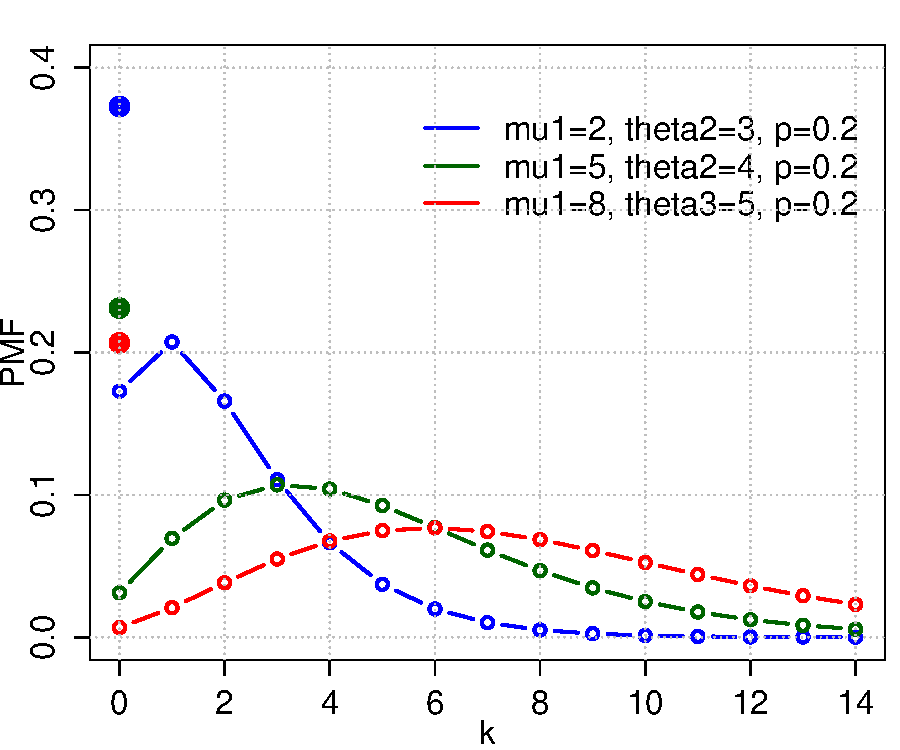
\includegraphics[width=70mm]{pics/ZINB_pmf_cdf.pdf}
 \caption{PDF and CDF of the ZINB distribution plotted using the provided R-code.}
 \label{fig:ZINBpdfcdf}
\end{figure}

\subsubsection*{Parameter: mean}

\noindent\begin{tabular}{p{2cm}cl}
\textbf{name} & & mean \\
\textbf{type} & & scalar \\
\textbf{symbol} & & $\mu$  \\
\textbf{definition} & & $\mu > 0$
\end{tabular}
\subsubsection*{Parameter: sizeParameter}

\noindent\begin{tabular}{p{2cm}cl}
\textbf{name} & & size parameter \\
\textbf{type} & & scalar \\
\textbf{symbol} & & $\theta$  \\
\textbf{definition} & & $-$
\end{tabular}
\subsubsection*{Parameter: probabilityOfZero}

\noindent\begin{tabular}{p{2cm}cl}
\textbf{name} & & probability of zero \\
\textbf{type} & & scalar \\
\textbf{symbol} & & $p$  \\
\textbf{definition} & & $0<p<1, p \in R$
\end{tabular}
\subsubsection*{Functions}

\smallskip \noindent \hspace{.2cm} \textbf{PMF} 
\begin{equation*}\begin{cases}
p + (1-p) \Big(\frac{\theta}{\theta + \mu} \Big)^{\theta} & \text{for } y = 0 \\ 
(1-p) \frac{\Gamma(\theta + y)}{\Gamma(a)\Gamma(y+1)} \Big(\frac{\theta}{\theta + \mu} \Big)^{\theta} 
\Big(\frac{\mu}{\theta + \mu} \Big)^{y} & \text{for } y > 0
\end{cases}\end{equation*}
\smallskip \noindent \hspace{.2cm} \textbf{PMF in R}  
\begin{verbatim}p + (1-p) * (theta/(theta + mu))^theta * (mu/(theta+mu))^y  for y=0
(1-p)*gamma(theta+y)/gamma(a)/gamma(y+1)*(theta/(theta+mu))^theta*(mu/(theta+mu))^y for y>0\end{verbatim}
\smallskip \noindent \hspace{.2cm} \textbf{CDF} 
\begin{equation*}-\end{equation*}
\smallskip\section*{ZeroInflatedPoisson} 

  \bigskip 

\begin{tabular}{p{2cm}cl}
\textbf{name} & & Zero-inflated Poisson (ID: 0000019)\\ 
 
\textbf{type} & & discrete \\ 

\textbf{variate} & & $k$, scalar \\ 

\textbf{support} & & $k \in \{0,1,2,3,\dots\}$
\end{tabular}

\begin{figure}[htb!]
\centering
  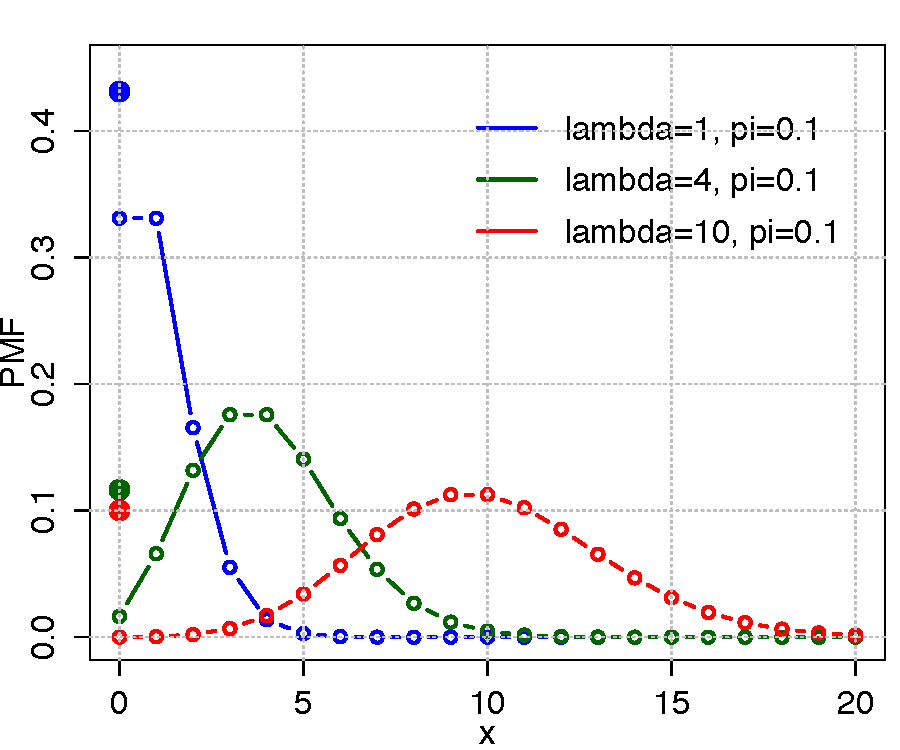
\includegraphics[width=70mm]{pics/ZIP_pmf.pdf}
 \caption{PMF of the ZIP distribution plotted using the provided R-code.}
 \label{fig:Poisson_pmf_cdf}
\end{figure}

\subsubsection*{Parameter: rate}

\noindent\begin{tabular}{p{2cm}cl}
\textbf{name} & & Poisson intensity \\
\textbf{type} & & scalar \\
\textbf{symbol} & & $\lambda$  \\
\textbf{definition} & & $\lambda \in R, \lambda > 0$
\end{tabular}
\subsubsection*{Parameter: probabilityOfZero}

\noindent\begin{tabular}{p{2cm}cl}
\textbf{name} & & probability of extra zeros \\
\textbf{type} & & scalar \\
\textbf{symbol} & & $\pi$  \\
\textbf{definition} & & $0<\pi<1, \pi \in  R$
\end{tabular}
\subsubsection*{Functions}

\smallskip \noindent \hspace{.2cm} \textbf{PMF} 
\begin{equation*}\begin{cases}
\pi + (1-\pi) e^{-\lambda}& \text{for } k = 0 \\ 
(1-\pi) e^{-\lambda} \frac{\lambda^k}{k!} & \text{for } k > 0
\end{cases}\end{equation*}
\smallskip \noindent \hspace{.2cm} \textbf{PMF in R}  
\begin{verbatim}pi + (1-pi)*exp(-lambda) if k=0\\
(1-pi)*exp(-lambda) * lambda^k/factorial(k)  if k>0\end{verbatim}
\smallskip \noindent \hspace{.2cm} \textbf{CDF} 
\begin{equation*}-\end{equation*}

\section{NEW STUFF}

%%\smallskip\section*{Gumbel} 
%\begin{figure}[htb!]
%\centering
%  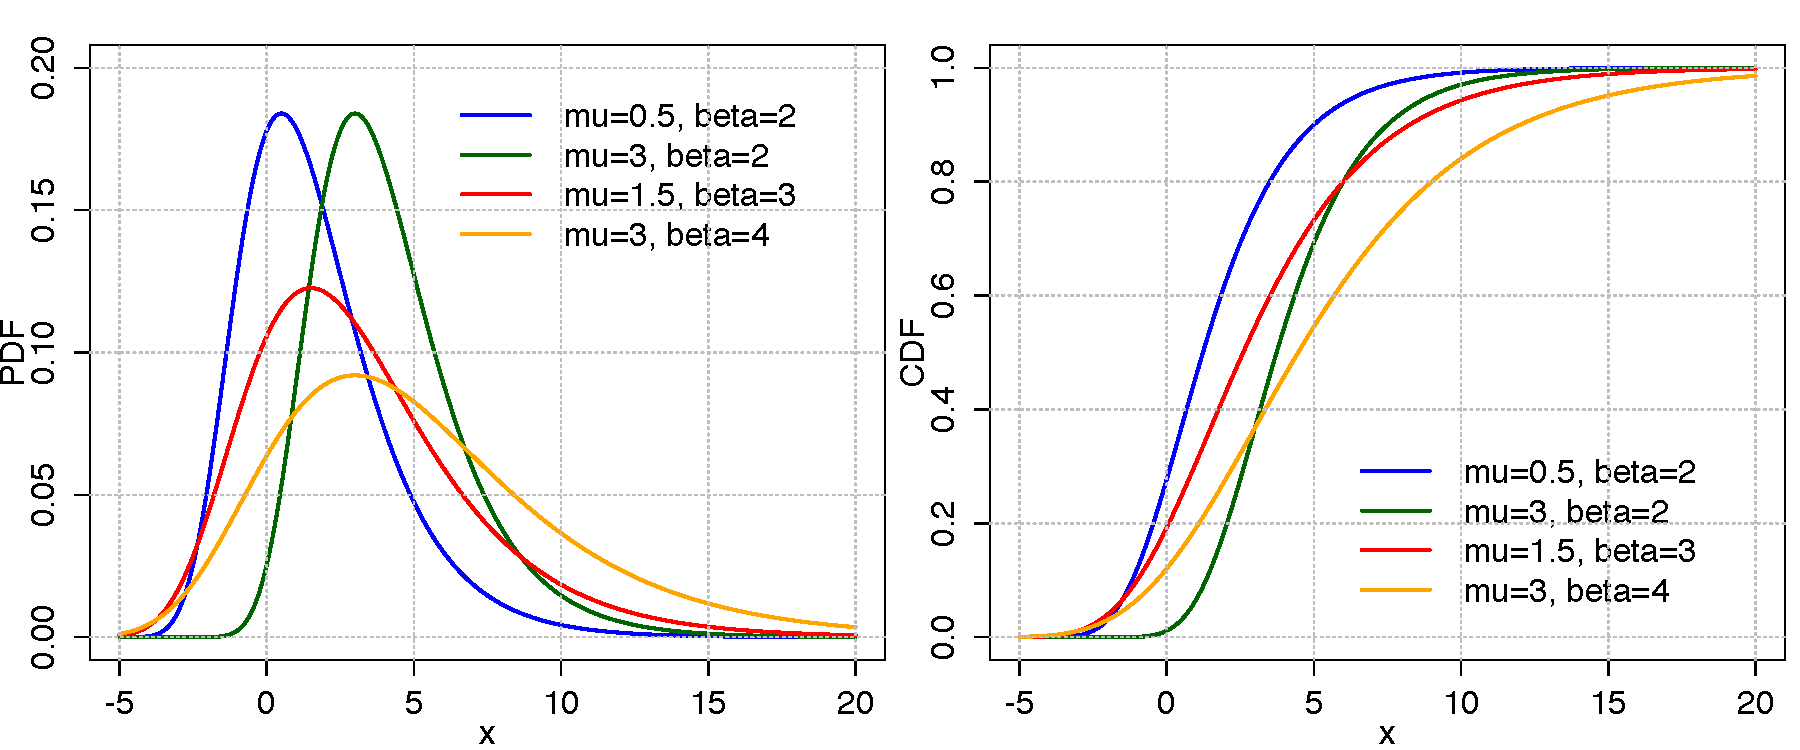
\includegraphics[width=140mm]{pics/Gumbel_pdf_cdf.pdf}
% \caption{PDF of the Gumbel distribution plotted using the provided R-code.}
% \label{fig:Gumbel_pdf_cdf}
%\end{figure}



Noncentral Chi-Square Distribution\\
Noncentral F Distribution\\
Noncentral t Distribution\\



